\documentclass[oneside]{scrbook}
\KOMAoptions{fontsize=11pt, paper=a4}     
\KOMAoptions{DIV=13}                      

\usepackage[utf8]{inputenc}               
\usepackage[T1]{fontenc}                  
\usepackage[varg]{txfonts}  			  %	Times-like fonts in support of mathematics
\usepackage[separate-uncertainty = true]{siunitx}   	  				  
\usepackage{enumitem}				      %	extra enumerate options

% \renewcommand{\familydefault}{\rmdefault} % font to sans serif

%import external graphics and where to find these
\usepackage{graphicx}					  
\graphicspath{{figs/}}

\RequirePackage[backend=biber, style=numeric]{biblatex}
\addbibresource{refs.bib}

\usepackage[hypertexnames=false]{hyperref}
% By default, hyperref creates internal links based on the counters. When counters are changed, the names may not be properly distinguishable internally.
\RequirePackage[all]{hypcap}

%There are a number of symbols defined inside txfonts that are also defined in amsmath
% so you can just make these available again
\let\iint\relax
\let\iiint\relax
\let\iiiint\relax
\let\idotsint\relax
\usepackage{amsmath}
\usepackage{physics}
\usepackage{mathtools}
\usepackage{braket}
\usepackage{slashed} % feynman slash notation
\usepackage{simplewick} % wick contraction
\usepackage{tikz}
\usepackage{tikz-feynman} % feynman diagrams
\usepackage{here} % figure[H]
\usepackage{cancel}
% \usepackage{cleveref}

% Externalizing plots
\usetikzlibrary{external}
\tikzexternalize[ prefix=tikz-figs/,
                  mode=list and make,
                  system call={ lualatex \tikzexternalcheckshellescape -halt-on-error -interaction=batchmode -jobname="\image" "\texsource"  || rm "\image.pdf"},
]

%restart footnotes every page
\usepackage{perpage}
\MakePerPage{footnote}
%symbols for footnotes
\usepackage[symbol]{footmisc}
\renewcommand{\thefootnote}{\fnsymbol{footnote}} % footnote mark with special symbols

% toprule and etc.
\usepackage{booktabs}

% Color
\usepackage{xcolor}
%%%%%%%%%%%%%%%%%%%%%%%%%% NEW COMMAND SECTION %%%%%%%%%%%%%%%%%%%%

%define equal
\newcommand{\defeq}{\vcentcolon =} 
\newcommand{\eqdef}{= \vcentcolon}
\newcommand{\euler}{\mathrm{e}}

%Lagrange density
\newcommand{\lag}{\mathcal{L}} 
%Hamiltonian density
\newcommand{\ham}{\mathcal{H}}
\usepackage{mathrsfs}
\newcommand{\hil}{\mathscr{H}}

%identity matrix
\usepackage{dsfont}
\newcommand{\id}{\mathds{1}}

\newcommand{\vecnab}{\pmb{\nabla}}
\newcommand{\vecx}{\pmb{x}}
\newcommand{\vecy}{\pmb{y}}
\newcommand{\veck}{\pmb{k}}
\newcommand{\vecp}{\pmb{k}}
\newcommand{\N}{\mathbb{N}}
\newcommand{\R}{\mathbb{R}}
\newcommand{\Co}{\mathbb{C}}
\newcommand{\D}{\mathcal{D}}
\newcommand{\M}{\mathcal{M}}
\newcommand{\diag}{\text{diag}}
\newcommand{\sgn}{\text{sgn}}
\newcommand{\cl}{\text{cl}}
\newcommand{\eff}{\text{eff}}
\newcommand{\SU}{\mathbf{SU}}
\newcommand{\SO}{\mathbf{SO}}
\newcommand{\SL}{\mathbf{SL}}
\newcommand{\Uni}{\mathbf{U}}

% command for neutrino or anti-neutrino
\newcommand{\nub}[1]{\nu_#1 (\bar{\nu}_#1)} 

% new unit
\DeclareSIUnit\year{yr}
%%%%%%%%%%%%%%%%%%%%%%%%%%%%% SETTINGS %%%%%%%%%%%%%%%%%%%%%%%%%%%%%%%%%%%%

\numberwithin{equation}{section}

% \setcounter{secnumdepth}{4}
\setcounter{tocdepth}{4}
%%%%%%%%%%%%%%%%%%%%%%%%%%%%%%%%%%%%%%%%%%%%%%%%%%%%%%%%%%%%%%%%%%

\title{Advanced Theoretical Particle Physics}
\author{Chenhuan Wang}
\date{\today}
\begin{document}
\maketitle
\tableofcontents

\setcounter{chapter}{-1}
\chapter{Preliminaries}
\section{Notations and conventions}
(mostly follow Peskin and Schroeder)

Metric
\begin{equation}
   g_{\mu\nu} = g^{\mu\nu} = \diag(+1, -1, -1, -1) \label{0.1}
\end{equation}

Scalar product of $4$-vectors $p_\mu, q_\mu$
\begin{equation*}
   p \cdot q = g_{\mu\nu} p^\mu q^\nu = p^\mu q_\mu
\end{equation*}
For momentum $p^\mu = (E_p, \pmb{p}); q^\nu = (E_q, \pmb{q})$
\begin{equation}
   p \cdot q = E_p E_q - \pmb{p}\cdot \pmb{q} \label{0.2}
\end{equation}

Use "natural units"
\begin{equation*}
   \hbar = c = 1
\end{equation*}

Pauli matrices
\begin{equation}
   \sigma_1 = \begin{pmatrix} 0 & 1 \\ 1 & 0 \end{pmatrix}; \quad
   \sigma_2 = \begin{pmatrix} 0 & -i \\ i & 0 \end{pmatrix}; \quad 
   \sigma_3 = \begin{pmatrix} 1 & 0 \\ 0 & -1 \end{pmatrix} \label{0.3}
\end{equation}

Dirac matrices in Dirac representation
\begin{equation}
   \gamma^0 = \begin{pmatrix} \id_2 & 0 \\ 0 & -\id_2 \end{pmatrix}; \quad
   \gamma^i = \begin{pmatrix} 0 & \sigma_i \\ -\sigma_i & 0 \end{pmatrix};\quad
   \gamma_5 = \begin{pmatrix} 0 & \id_2 \\ \id_2 & 0 \end{pmatrix}
   \label{0.5}
\end{equation}

Chiral projectors
\begin{equation}
   P_{L, R} = \frac{1}{2} (1 \mp \gamma_5) \label{0.6}
\end{equation}

Dirac slash
\begin{equation}
   \slashed{p} = p_\mu \gamma^\mu
   \label{0.7}
\end{equation}
for all $4$-vector $p_\mu$.

Lorentz boost
\begin{equation}
   p'_\mu = \Lambda_\mu^\nu p_\nu
   \label{0.8}
\end{equation}
for all $4$-vector $p_\mu$ and with $\det \Lambda = 1$. E.g.~boost in $z$-direction with velocity $\beta = v/c$
\begin{equation}
   \Lambda = \begin{pmatrix} \gamma & 0 & 0 & -\beta\gamma \\ 0 & 1 & 0 & 0 \\ 0 & 0 & 1 & 0 \\ -\beta \gamma & 0 & 0 & \gamma \end{pmatrix}, \gamma = \frac{1}{\sqrt{1-\beta^2}}
   \label{0.9}
\end{equation}

Field operators (in $4$ dimensions): for bosons scalar $\phi$ and vectors $A_\mu$ with mass dimension $1$
\begin{equation*}
   [\phi] = [A_\mu] = \si{\giga\eV} 
\end{equation*}
For fermion $\psi$, mass dimension $3/2$
\begin{equation*}
   [\psi] = \si{\giga\eV}^{3/2}
\end{equation*}

Polarization vector $\epsilon_\mu$ is dimensionless.

$4$-component spinors $u(p)$, $v(p)$ have mass dimensions $1/2$
\begin{equation}
   \bar u (p) u (p) = - \bar v (p) v(p) = 2m = 2 \sqrt{p^2} \label{0.11}
\end{equation}

Summation convention is to sum over repeated upper/lower indices.

\section{The Standard Model}
Based on gauge group
\begin{equation}
   G_\text{SM} = \SU(3)_C \times \SU(2)_L \times \Uni(1)_Y
   \label{0.12}
\end{equation}

Particle content
\begin{equation*}
\begin{tabular}{ccc ccc}
   \toprule
   Particle & $\SU(3)$ rep. & $\SU(2)$ rep. & $I_3$ & $Y$ & Spin \\
   \midrule
   gluon $g$ & $8$ & $1$ & $0$ & $0$ & $1$ \\ 
   $W$ boson & $1$ & $3$ & $\pm 1, 0$ & 0 & $1$ \\
   $B$ boson & $1$ & $1$ & $ 0$ & 0 & $1$ \\
   \midrule 
   $u_L, c_L, t_L$ & $3$ & $2$ & $+ \frac{1}{2}$ & $+ \frac{1}{6}$ & $\frac{1}{2}$ \\
   $d_L, s_L, b_L$ & $3$ & $2$ & $- \frac{1}{2}$ & $+ \frac{1}{6}$ & $\frac{1}{2}$ \\
   $u_R, c_R, t_R$ & $3$ & $1$ & $0$ & $+ \frac{2}{3}$ & $\frac{1}{2}$ \\
   $d_R, s_R, b_R$ & $3$ & $1$ & $0$ & $- \frac{1}{3}$ & $\frac{1}{2}$ \\
   \midrule
   $e_L, \mu_L, \tau_L$ & $1$ & $2$ & $-\frac{1}{2}$ & $-\frac{1}{2}$ & $\frac{1}{2}$ \\
   $\nu_{e_L}, \nu_{\mu_L}, \nu_{\tau_L}$ & $1$ & $2$ & $+\frac{1}{2}$ & $- \frac{1}{2}$ & $\frac{1}{2}$ \\
   $e_R, \mu_R, \tau_R$ & $1$ & $1$ & $0$ & $-1$ & $\frac{1}{2}$ \\
   \midrule
   Higgs boson $\phi$ & $1$ & $2$ & $\pm \frac{1}{2}$ & $+\frac{1}{2}$ & $0$ \\
   \bottomrule
\end{tabular}
\end{equation*}

In this convention
\begin{equation}
   Q = I_3 + Y \label{0.13}
\end{equation}

Lagrangian
\begin{align}
      \lag_\text{SM} &= \sum_\text{fermions} \bar\psi_i \slashed{D} \psi_i  &&\text{matter kinetic term}\notag \\
                     &- \frac{1}{4} \left[ \sum_{a=1}^8 F_{\mu\nu}^a F_a^{\mu\nu} + \sum_{k=1}^3 W_{\mu\nu}^k W^{\mu\nu}_k + B_{\mu\nu} B^{\mu\nu} \right]  &&\text{pure gauge}\notag \\
                     &+ \left( D_\mu \phi \right)^\dagger D^\mu \phi && \text{Higgs kinetic term}\notag\\
                     &- m^2 \phi^\dagger \phi - \frac{\lambda}{2} (\phi^\dagger \phi)^2 && \text{Higgs potential} \notag \\
                     &- \left[ \sum_{j=1}^3 f_j^{(l)} \overline{e^-}_{jR} \phi^\dagger L_{jL} + \sum_{j,l} f_{jk}^{(d)} \bar d_{jR} \phi^\dagger \cdot q_{kL} - \sum_{j,k=1}^3 f_{jR}^{(u)} \bar u_{jR} \phi \cdot q_{L k} + h.c. \right] && \text{Yukawa interactions}
   \label{0.14}
\end{align}

\begin{equation}
   D_\mu = \partial_\mu + \underbrace{i g_s \frac{\lambda_a}{2} A_{\mu a}}_{\text{only for quarks}} + \underbrace{i g \frac{\tau_l}{2} W_{l \mu}}_{\text{only for $\SU(2)$ doublets}} + i g' \hat{Y} B_\mu \label{0.15}
\end{equation}
with $\hat {Y} \psi = Y_\psi \psi$.

Field strength tensors
\begin{align}
   F_{\mu\nu}^a &= \partial_\mu A^a_\nu - \partial_\nu A_\mu^a + g_s f^{abc} A_\mu^b A_\nu^c \label{0.15} \\
   W_{\mu\nu}^a &= \partial_\mu W_\nu^i - \partial_\nu W_\mu^i + g \epsilon^{ijk} W_\mu^j W_\nu^k \label{0.16} \\
   B_{\mu\nu} &= \partial_\mu B_\nu - \partial_\nu B_\mu \label{0.17}
\end{align}

Doublets are
\begin{equation}
   \begin{split}
      L_{1L} &= \begin{pmatrix} \nu_e \\ e^- \end{pmatrix}_L, \quad L_{2L} = \begin{pmatrix} \nu_\mu \\ \mu^- \end{pmatrix}_L, \quad L_{3L} = \begin{pmatrix} \nu_\tau \\ \tau^- \end{pmatrix}_L, \\
      q_{1L} &= \begin{pmatrix} u \\ d \end{pmatrix}_L, \quad q_{2L} = \begin{pmatrix} c \\ s\end{pmatrix}_L, \quad q_{3L} = \begin{pmatrix} t \\ b\end{pmatrix}_L, \quad \phi = \begin{pmatrix} \phi^\dagger \\ \phi^0 \end{pmatrix}
   \end{split}
   \label{0.18}
\end{equation}

\begin{equation}
   \phi^\dagger \cdot L_{1L} = \phi^{\dagger *} \nu_{eL} + \phi^{0 *} e^-_L; \quad \phi \cdot q_{1L} = \phi^\dagger d_L - \phi^0 u_L \label{0.19}
\end{equation}

\chapter{Neutrino Masses}
\section{Neutrino Oscillations}
\subsection{Evidence and Motivation}
It is based on the observation that neutrinos disappear, or change flavour between source and detector!

\paragraph{Solar neutrinos} are produced by following mechanisms (all $\beta$-decays!)
\begin{itemize}
   \item $pp$-neutrinos: produced by $4p \rightarrow {}^4 \text{He} + 2 e^+ + 2 \nu_e$; $E_{\nu_e} < \SI{0.42}{\mega \eV}$; flux $\phi= \SI{6e10}{\cm\tothe{-2}\s\tothe{-1}}$
   \item $pep$-neutrinos: produced by $p+e^-+p \rightarrow d + \nu_e$; $E_{\nu_e} < \SI{1.44}{\mega \eV}$; flux $\phi=\SI{0.015e10}{\cm\tothe{-2}\s\tothe{-1}}$
   \item $Be$-neutrinos: produced by ${}^{7}\text{Be} + e^- \rightarrow {}^7 Li + \nu_e$; $E_{\nu_e} < \SI{0.86}{\mega \eV}$; flux $\phi=\SI{0.48e10}{\cm\tothe{-2}\s\tothe{-1}}$
   \item $B$-neutrinos: produced by ${}^8 \text{B} \rightarrow {}^8 \text{Be} + e^+ + \nu_e$; $E_{\nu_e} = \SI{14}{\mega \eV}$; flux $\phi=\SI{0.5e7}{\cm\tothe{-2}\s\tothe{-1}}$
\end{itemize}
Note that only electron neutrinos are produced!

\begin{figure}[htpb]
   \centering
   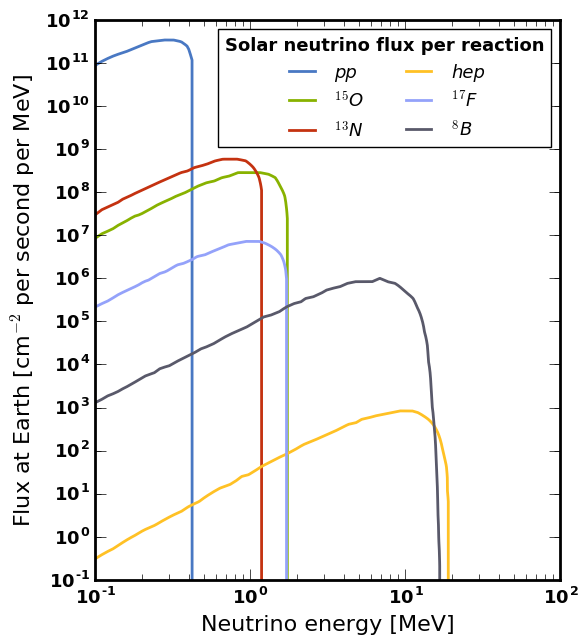
\includegraphics[width=0.5\linewidth]{Solar_neutrino_flux_spectrum.png}
   \caption{Solar neutrino flux spectrum\cite{wiki:solarNu}}%
   \label{fig:}
\end{figure}

Detection of neutrinos can be achieved by
\begin{itemize}
   \item Chemical via $(A,Z) + \nu_e \rightarrow (A,Z+1) + e^-$. Extract new element using chemistry and observe its decay. Used for Cl and Ga targets.
   \item Reverse electron capture $\nu_e + n \rightarrow e^- + p $. Detect $e^-$ in Cherenkov scintillation detection.
   \item Elastic scattering off electron $\nu + e^- \rightarrow \nu + e^-$. Detect scattered $e^-$, and mostly used for $\nu_e$ (CC-contribution).
   \item Scattering off deuterium $\nu + d \rightarrow \nu + n + p$. Detect free neutron. Here all neutrinos contribute equally. 
\end{itemize}

Results are
\begin{itemize}
   \item Between $1/3$ and $2/3$ of produced in the Sun (known from Solar energy output and solar modelling) do not participate in CC reactions ("disappear").
   \item Total active neutrino flux measured at Sudbury Neutrino Observatory (SNO) does agree with predictions.
\end{itemize}
So we conclude $\nu_e \rightarrow \nu_\mu, \nu_\tau$.

\paragraph{Atmospheric neutrinos} are produced by hardonic shower from cosmic rays hitting atmosphere. 
\begin{align}
   \pi^\pm &\rightarrow \mu^\pm + \nu_\mu (\bar{\nu}_\mu) \\
   \mu^\pm &\rightarrow e^\pm + \nu_e(\bar{\nu}_e) + \nu_\mu(\bar{\nu}_\mu)
\end{align}
We expect two $\nu_\mu (\bar{\nu}_\mu)$ for each $\nu_e (\bar{\nu}_e)$ at $E \lessapprox \SI{10}{\giga \eV}$. But roughly equal numbers of $\nu_e$ and $\nu_\mu$ are observed via $\nu_l + N \rightarrow l + X$ with $l=e,\mu$. The interpretation is that mostly $\nu_\mu (\bar{\nu}_\mu) \rightarrow \nu_e (\bar{\nu}_e)$.

\paragraph{Reactor neutrinos} are produced by nuclear fission where the remnants are unstable because of "too many neutrons"
\begin{align}
   (A,Z) \rightarrow (A, Z+1) + e^- + \bar{\nu}_e 
\end{align}
And $E_{\bar{\nu}_e} \sim \si{\mega \eV}$. Its detection is done by scintillation detectors $\bar{\nu}_e + p \rightarrow e^+ + n$. KAMLand experiment found significant deficit of $\bar{\nu}_e$ at $L \sim \SI{100}{\kilo \m}$. At Daya Bay and Reno experiments, it is found few percent deficit at $L\sim \SI{1}{\kilo\m}$.

\paragraph{Neutrino beams} are produced by meson beam decay. Mostly $\nu_\mu (\bar{\nu}_\mu)$ from $\pi^\pm$ decay. However, there is some contamination of $\nub{e}$, also from Kaon decay $K^\pm \rightarrow \pi^0 e^\pm \nub{e} $. K2K experiment (Japan) and MINOS experiment (USA) find significant deficits at $L\sim \SI{100}{\kilo\m}$ and $E_\mu \sim \SI{1}{\giga \eV}$. Interpretation is mostly $\nu_\mu \rightarrow \nu_\tau$.

All together the most likely interpretation is neutrino flavor oscillations!

\subsection{Theory}
Suppose that neutrinos have non-trivial mass matrix, as quarks do. Their mass eigenstates $v_i$ are linear combinations of flavour eigenstates $\nu_\alpha$
\begin{align}
   \nu_\alpha &= \sum_{j} U_{\alpha j} \nu_j, \label{1.1} \\
   \nu_i &= \sum_{\alpha} U^*_{\alpha j} \nu_\alpha.
\end{align}
Obviously $U$ is unitary matrix
\begin{align*}
   \sum_{j} U_{\alpha j} U^*_{\beta j} = \delta_{\alpha \beta}, \quad
   \sum_{\alpha} U_{\alpha j} U^*_{\alpha k} = \delta_{jk}.
\end{align*}

Flavour is defined by gauge i.a., in particular by CC interactions of charged leptons. CC interactions vertex involves $e$ and $\nu_e$ as well.

For stable neutrinos, the mass eigenstates are orthonormal
\begin{align}
   \braket{ \nu_i (t) | \nu_j (t)} = \delta_{ij}.
\end{align}
Representing the mass eigenstates in terms of flavour eigenstates with equation (\ref{1.1})
\begin{align}
   \sum_{\alpha, \beta} U^*_{\alpha j} U_{\beta i} \braket{\nu_\beta (t) | \nu_\alpha (t)} &= \delta_{ij}, \notag \\
   \sum_{\alpha, \beta, i, j} U^*_{\alpha j} U_{\gamma j} U_{\beta i} U^*_{\delta i} \braket{\nu_\beta (t ) | \nu_\alpha (t)} &= \sum_{i,j} \delta_{ij} U_{\gamma j} U^*_{\delta i}, \notag \\
   \sum_{\alpha, \beta, i, j} \delta_{\alpha \gamma} \delta_{\beta \delta} \braket{\nu_\beta(t) | \nu_\alpha(t)} &= \sum_{i} U_{\gamma i} U^*_{\delta i} = \delta_{\gamma \delta}. \label{1.3}
\end{align}
On the second line, $\sum U_{\gamma j} U^*_{\delta i}$ is multiplied to both sides. Flavour states are also orthonormal!

\paragraph{Flavour transition amplitudes} using plane waves (QM treatment). Produce flavour $\alpha$ at $\pmb{x} = 0$ and $t=0$. We want to find out amplitude for transition to flavour $\beta$ at $\pmb{x}, t$.
\begin{align}
   A_{\alpha \rightarrow \beta} (t, \pmb{x}) &= \braket{\nu_\beta (t,\pmb{x}) | \nu_\alpha(0)} \\
                                             &= \braket{\nu_\beta (0)| \exp[-i(\hat{H}_\text{free} t - \hat{\pmb{p}} \cdot \pmb{x})] | \nu_\alpha (0)} \notag
\end{align}
Since $\nu_\alpha$ is not mass eigenstate, it is not eigenstate of $\hat{H}_\text{free}$ either. Remember in QM, $\hat{p}\psi = -i \partial_x \psi$. Use equation (\ref{1.1}) and assume plane wave (momentum eigenstate) in second step
\begin{align}
   A_{\alpha \rightarrow \beta } (t, \pmb{x}) &= \sum_{j} \braket{\nu_\beta (0)| \exp[-i(\hat{H}_\text{free} t - \hat{\pmb{p}} \cdot \pmb{x})] U_{\alpha j}| \nu_j (0)} \notag \\
                                              &= \sum_{j} \braket{\nu_\beta (0)|U_{\alpha j} \exp[-i(E_j t - \pmb{p}_j \cdot \pmb{x})] | \nu_j (0)} \notag \\
                                              &\stackrel{(\ref{1.1})}{=} \sum_{j,\gamma} \braket{\nu_\beta(0) | U_{\alpha j} \exp[-i(E_j t - \pmb{p}_j \cdot \pmb{x})] U^*_{\gamma j} | \nu_\gamma (0)} \notag \\
                                              &\stackrel{(\ref{1.3})}{=} \sum_j U_{\alpha j} U^*_{\beta j} \exp[-i(E_j t - \pmb{p}_j \cdot \pmb{x})] \label{1.6}
\end{align}

The transition probability
\begin{align}
   P_{\alpha \rightarrow \beta}(t, \pmb{x}) &= \left| A_{\alpha \rightarrow \beta} (t, \pmb{x}) \right|^2, \notag \\
                                            & = \sum_{k,j} U_{\alpha j} U^*_{\beta j} \exp[-i(E_j t - \pmb{p}_j \cdot \pmb{x})] U_{\alpha k} U^*_{\beta k} \exp[i(E_k t - \pmb{p}_k \cdot \pmb{x})] \notag \\
                                            &= \sum_{k,j} U_{\alpha j} U^*_{\alpha k} U_{\beta k} U^*_{\beta j} \exp[-i((E_j - E_k) t - (\pmb{p}_j - \pmb{p}_k) \cdot \pmb{x})] \label{1.7}
\end{align}
Note that off-diagonal ($k\neq j$) contributions have non-trivial phase factor and it leads to oscillations!

\paragraph{Example} with 2 states. The transformation matrix can easily be parametrized by a rotation $\theta$
\begin{align}
   U = U^* = \begin{pmatrix} \cos(\theta) & \sin (\theta) \\ -\sin (\theta) & \cos (\theta) \end{pmatrix} \label{1.8}
\end{align}
Then the probability is
\begin{align}
   P_{1\rightarrow 2} &= \cos^2(\theta) \sin^2(\theta) + \sin^2(\theta) \cos^2(\theta) - \sin^2(\theta) \cos^2(\theta)  \exp[-i((E_2 - E_1) t - (\pmb{p}_2 - \pmb{p}_1) \cdot \pmb{x})], \notag \\
                      &\quad - \sin^2(\theta) \cos^2(\theta) \exp[-i((E_1 - E_2) t - (\pmb{p}_1 - \pmb{p}_2) \cdot \pmb{x})], \notag \\
                      &= \cos^2(\theta) \sin^2(\theta) \left[ 2 - 2 \cos((E_2 - E_1)t - (\pmb{p}_2 - \pmb{p}_1)\cdot \pmb{x}) \right], \notag \\
                      &= \sin^2(2\theta) \sin^2[((E_2 - E_1)t - (\pmb{p}_2 - \pmb{p}_1)\cdot \pmb{x})/2]. \label{1.9}
\end{align}
Note  that one needs non-trivial mixing angle ($\theta \neq 0, \pi/2$) and non-zero mass difference for oscillations! To see the latter, expand phase around average momentum $\pmb{p}$ and assume $E \gg m $ (ultra-relativistic limit, reasonable for neutrinos!). Treat the problem in $1$-dimension
\begin{align*}
   E_1 &= \sqrt{m_1^2 + \pmb{p}_1^2}, \\
       &= \sqrt{m_1^2 + p^2 + 2p(p_1 - p) + (p_1 - p)^2}, \\
       &= \frac{m_1^2}{2p} + p  + (p_1 - p) + \order{(p_1-p)^2},
\end{align*} 
\begin{align}
   P_{1\rightarrow 2} = \sin^2(2\theta) \cdot \sin^2 \left[\frac{m_1^2 - m_2^2}{4p}t + (t-x) \frac{p_1-p_2}{2} \right] \label{1.10}
\end{align}
Note
\begin{itemize}
   \item Assumed $t_1 = t_2$ exactly
   \item standard treatment also assumes $t=x$, i.e. classical propagation, or $p_1 = p_2$ (which $E_1 \neq E_2$, since mass eigenstates must be on-shell!)
\end{itemize}

\begin{align}
   P_{1\rightarrow 2} = \sin^2(2\theta) \cdot \sin^2 \left( \frac{\pi x}{L_\text{osc}} \right), \label{1.11}
\end{align}
with oscillation length
\begin{align*}
   L_\text{osc} = \frac{4\pi p}{ \left| m_1^2 - m_2^2 \right| } \approx \frac{4\pi E}{ \left| m_1^2 - m_2^2 \right| }.
\end{align*}
We observe that one needs smaller $E$ to probe smaller $\delta m^2$ at fixed $x$. For more than two states, the expression is similar 
\begin{align}
   L_{ij, \text{osc}} = \frac{4\pi E}{ \left| m_i^2 - m_j^2 \right| }. \label{1.13}
\end{align}

Oscillations have been seen in atmospheric neutrinos! (SuperK, $\sim 1998$) The result can further corrected by QFT\cite{Beuthe_2003}. Phenomenological aspect can be found in \cite{Esteban_2019}. We need two large mixing angles, one small but non-zero. There is probably non-trivial CP-violation.
\begin{align*}
   \Delta m^2_{21} &= (\num{7.4 +- 0.2}) \cdot 10^{-5} \si{\eV \tothe{2}} \\
   \Delta m^2_{31} &= (\num{2.52 +- 0.03})\cdot 10^{-3}\si{\eV \tothe{2}}
\end{align*}
From cosmology, we know $\sum_j m_{\nu_j} \lessapprox \SI{0.5}{\eV}$. So the heaviest neutrino  $m_{\nu_3} \in [\SI{0.04}{\eV}, \SI{0.2}{\eV}] $, much smaller than $m_e$!

\section{Generation of Small Neutrino Masses}
\paragraph{Simplest way}
conceptually is to treat $\nu$'s like charged fermions and introduce $\SU(2)$ singlet right-handed neutrino.
\begin{align}
   \lag_{\text{Yuk}} \supset - \sum_{j,k=1}^{3} \left[ f^{(l)}_{jk} \overline{e^-}_{jR} \phi^\dagger L_{k L} - f^{(\nu)}_{jk} \textcolor{blue}{\bar{\nu}_{jR}} \phi L_{kL} \right] + h.c. \label{1.36}
\end{align}
The resulted mass matrix $(M_l)_{jk}f_{jk}^{(l)} v$ is in general not diagonal. So we need matrix $U_{L,R}$ to diagonalize it
\begin{align}
   l_R^{(p)} = U_R^{(l)}l_R; \quad l_L^{(p)} = U_L^{(l)}l_L  \notag \\
   \overline{l}_R M_l l_L = \overline{l}^{(p)}_R U^{(l)}_R M_l U^{(l)\dagger}_L l_L^{(p)} \label{1.37}
\end{align}

Also transforms $\nu$ in Yukawa terms
\begin{align}
   \lag_{\nu-\text{Yukawa}} = \overline{\nu}_R f^{(\nu)} U_L^{(P)\dagger} \phi L_L.
\end{align}
It gives Dirac mass term; $\nu_R$ is SM singlet ("sterile" neutrino).

To diagonalize $\nu$ mass matrix
\begin{align}
   \nu_R^{(p)} = U_R^{(\nu)} \nu_R, \quad \nu_L^{(p)} = U_L^{(\nu)} U_L^{(e)\dagger}\nu_L
\end{align}

Only $\nu_L$ have gauge so we can only probe 
\begin{align}
   U_{MNS} = \left[ U_L^{(\nu)} U_L^{(l)\dagger} \right]^\dagger = U_L^{(l)} U_L^{(\nu)\dagger}
\end{align}
It is completely analogous to KM matrix in SM.

Drawback is that this mechanism cannot explain $m_{\nu_i} < \SI{1}{\eV}$ with Higgs VEV $v =\SI{175}{\giga\eV}$ and we need $|f^{(\nu)}| < \num{1e-11}$! C.f. to known Yukawas: $f_e \sim \num{3e-6}$, \dots, $f_\tau \approx 1$. So why are $f^{(\nu)}$ so tiny?

\paragraph{Most economical scheme} is via Majorana masses for $\nu_L$ and no sterile neutrinos $\nu_R$!
\begin{align}
   \lag_{\nu-\text{mass}} &= -\frac{1}{2} \sum_{j,k=1}^3 \overline{L^C_{Lj}} \phi \frac{\kappa_{jk}}{M} L_{Lk} \phi  \label{1.41} \\
                          & \stackrel{\phi\rightarrow v}{\longrightarrow} - \frac{v^2}{2M} \sum  \overline{\nu^C_{Lj}} \kappa_{jk} \nu_{Lk} \notag 
\end{align}
Here $L_L \phi$ is $\SU(2) \times \Uni(1)_\text{Y}$ invariant ($Y(\phi)=+1$ and $Y(L)=-1$).
Charge conjugate antiparticle is right-handed field with hypercharge $+\frac{1}{2}$
\begin{align}
   L_L^C = C \overline{L_L}^T.
\end{align}

Charge conjugation matrix $C$ satisfies
\begin{subequations}
   \label{1.42}
\begin{align}
   C^\dagger &= C^{-1}, \label{1.42a}\\
   C^T &= -C,  \label{1.42b}\\
   C \Gamma^T C^{-1} &= \eta_\Gamma \Gamma \label{1.42c},
\end{align}
\end{subequations}
with $\eta_\Gamma = +1 $ for $\Gamma \in \{\id, \gamma_5, \gamma_\mu \gamma_5\}$ and $\eta_\Gamma = -1$ for $\Gamma \in \{\gamma_\mu, \sigma_{\mu\nu}\}$.

Neutrino mass term in equation (\ref{1.41}) does not require new field, but is not renormalizable, since field operators have mass dimension $5$. So in order to keep $\kappa_{jk}$ dimensionless, $1/M$ is needed.

Majorana masses are
\begin{align}
   (m_\nu)_{jk} = \kappa_{jk} v^2 / M . \label{1.43}
\end{align}
Only know large mass scale is (reduced) Planck scale $M_p \simeq \SI{2.4e18}{\giga \eV}$ with $|\kappa_{jk}| \sim \order{1}$. Then $m_{\nu_i} \sim \SI{1e-5}{\eV}$ too small! Need new scale below Planck scale $M \sim \num{1e11} \cdots \SI{1e14}{\giga \eV}$.

Dirac mass term in equation (\ref{1.36}) violates in general lepton favour, but total lepton number is conserved! Hence it allows 
\begin{align}
   \begin{split}
      \mu^- &\rightarrow e^- + \gamma  \\
      \mu^- &\rightarrow e^- + e^+ + e^-
   \end{split} \label{1.44}
\end{align}
But it forbids $0\nu \beta \beta$-decay
\begin{align}
   (A,Z) \rightarrow (A,Z+2) + e^- + e^-. \label{1.45}
\end{align}
Ordinary $\beta\beta$-decay 
\begin{align}
   (A,Z) \rightarrow (A,Z+2) + e^- +e^- + \overline{\nu}_e+  \overline{\nu}_e,
\end{align}
is always allowed but the phase space is suppressed.

\paragraph{Majorana masses}
First simplify the charge conjugate antiparticle fields.
\begin{align}
    \overline{\nu^C_{Lj}} &= \overline{(C \overline{\nu}^T_{Lj})} \notag\\
                         &= \overline{ (C (\nu^\dagger_{Lj} \gamma_0)^T)} \notag\\
                         &= \overline{(C \gamma_0^T \nu_{Lj}^*)} \notag\\
                         &= (C \gamma_0^T \nu_{Lj}^*)^\dagger \gamma_0  \notag\\
                         &\stackrel{\ref{1.42a}}{=} \nu_{Lj}^T \gamma_0^* C^{-1}\gamma_0 \notag\\
                         &= \nu_{Lj}^T C^{-1} C \gamma_0^T C^{-1} \gamma_0 \notag\\
                         &\stackrel{\ref{1.42c}}{=} - \nu_{Lj}^T C^{-1} \gamma_0 \gamma_0 \notag\\ 
\Rightarrow    \overline{\nu^C_{Lj}}                     &= - \nu_{Lj}^T C^{-1} \label{1.46}
\end{align}

Mass term must be symmetric in flavour space!
\begin{align}
   \sum_{j,k} \overline{\nu^c_{Lj}} \kappa_{jk} \nu_{Lk} &\stackrel{!}{=} \sum_{j,k} \left( \overline{\nu^c_{Lj}} \kappa_{jk} \nu_{Lk} \right)^T \notag \\ 
   \text{RHS} &= - \sum_{j,k} \nu^T_{Lk} \kappa_{jk} \overline{\nu^c_{Lj}}^T \stackrel{\ref{1.46}}{=} \sum_{j,k} \nu_{Lk}^T \kappa_{jk} C^{-1 \; T} \nu_{Lj} \notag \\
              &\stackrel{\ref{1.42b}}{=} - \sum_{j,k} \nu_{Lk}^T C^{-1} \kappa_{jk} \nu_{Lj} \stackrel{\ref{1.46}}{=} \sum_{j,k} \overline{\nu^c_{Lk}} \kappa_{jk} \nu_{Lj} \notag \\
   \Rightarrow \kappa_{jk} &= \kappa_{kj}  \label{1.47}
\end{align}
Majorana mass matrix need not be hermitian!

The mass matrix can be diagonalized with single unitary matrix. In general,
\begin{equation}
   m = U_R M U_L^\dagger,
\end{equation}
with $m$ diagonal and $\in \R^{\geq 0}$ and $M$ non-diagonal. Then
\begin{align}
   M &= U_R^\dagger m U_L, \label{1.49}  \\
   M M^\dagger &= U_R^\dagger m U_L U_L^\dagger m U_R = U_R^\dagger m^2 U_R. \label{1.50}
\end{align}
Majorana mass matrix is symmetric
\begin{equation}
   M^T = U_L^T m U_R^* = M. 
\end{equation}
Thus
\begin{align}
   M M^\dagger &= M^T M^{T\dagger} = U_L^T m U_R^* U_R^T m U_L^* = U_L^T m^2 U_L^*, \notag \\
   \stackrel{\ref{1.50}}{\Longrightarrow}U_R^\dagger m^2 U_R &= U_L^T m^2 U_L^*, \notag \\
   U_L^* U_R^\dagger m^2 &= m^2 U_L^* U_R^\dagger, \notag \\
   \comm{U_L^* U_R^\dagger}{m^2} &= 0. \label{1.50.1}
\end{align}
Thus $U_L^* U_R^\dagger$ must be diagonal and unitary
\begin{align*}
   U_L^* U_R^\dagger = \diag(e^{2i\alpha_1}, e^{2i\alpha_2}, \dots) = S,
\end{align*}
with $\alpha_i \in \R$. Follow this
\begin{align}
   U_L^* = S U_R, \quad U_L = S^* U_R^*, \notag \\
   \stackrel{\ref{1.49}}{\Longrightarrow} M = U_R^\dagger m S^* U_R^* \stackrel{\ref{1.50.1}}{=} U^{\dagger} m U^*. \label{1.51}
\end{align}
with $U = S^{1/2} U_R $.  Thus
\begin{equation}
   m = U M U^T, \label{1.52}
\end{equation}
is required for consistency, since Majorana mass matrix is multiplied with the same field left and right. Note that we will meet Majorana masses and Majorana spinors again!

%%%%%%%%%%%5 Lecture 5a

\paragraph{See-Saw Mechanism} a renormalizable model for (\ref{1.41}). Introduce $\nu_R$ gauge single field, as in (\ref{1.41}), with additional Majorana mass term for them
\begin{equation}
   \lag_{\nu_R\text{-mass}} = -\frac{1}{2} \overline{\nu^c_R} M_R \nu_R^c + h.c. \label{1.53}
\end{equation}
This mass term is gauge invariant for \underline{any} $M_R$ and $\nu_R$ can be very heavy! 

Equations (\ref{1.36}) and (\ref{1.51}) can be written as
\begin{align}
   \lag_{\nu\text{-mass}} &= - \frac{1}{2} \overline{n_L^c} M n_L, \label{1.54a}
   \shortintertext{with $N_L + N_R$-component vector } 
   n_L &= (\nu_{L1},\dots, \nu_{L N_L},\nu^c_{R 1}, \dots, \nu^c_{R N_R})^T. \label{1.54b}
\end{align}

$M$ is Majorana mass matrix and symmetric
\begin{equation}
   M = \begin{pmatrix} 0 & M_D^T \\ M_D & M_R \end{pmatrix}  , \label{1.55}
\end{equation}
where each entry is a $3\times 3$ matrix. $M_D^T$ comes from (\ref{1.36}) and $M_R$ from (\ref{1.53}). It is used that $n_{L, N_L+i}^c = \nu^i_R$ ($\nu_R^c$ is left-handed and $\nu_L^c$ is right-handed).

Digitalization of (\ref{1.55}) using (\ref{1.52}) $m_\diag = U M U^T$
\begin{align*}
   \lag_{\nu\text{-mass}} = - \frac{1}{2} \overline{n^c_L} U^\dagger U M U^T U^* n_L + h.c.
\end{align*}
Transform to mass eigenstates 
\begin{align}
   n_L^{(p)} &= U^* n_L  \label{1.57}\\
   \lag_{\nu\text{-mass}} &= -\frac{1}{2} \overline{n^{(p)c}_L} m n_L^{(p)} + h.c. \notag
\end{align}
Introduce Majorana state
\begin{equation}
   \chi = n_L^{(p)} + \left(n_L^{(p)}\right)^c, \label{1.58}
\end{equation}
as combination of left- and right-handed fields. Then the mass term becomes
\begin{equation}
   \lag_{\nu\text{-mass}} = - \frac{1}{2} \sum_{k=1}^{N_L + N_R} m_k \overline{\chi_k} \chi_k. \label{1.59}
\end{equation}
Eigenstates are Majorana states. Two Majorana states with equal masses and opposite behaviour under $CP$ can be combined into a single Dirac state.

Interesting limit of (\ref{1.55}) elements of $M_R \gg$ elements of $M_D$. The heavy $\nu_R$ field can be integrated out (see homework) !

There are several ways to achieve this. 
\begin{itemize}
   \item approximately \textit{diagonalize} (\ref{1.55}) 
   \item solving \textit{equation of motion} 
   \item re-summed $\nu_L$ propagator, treating $M_D$ as perturbation
\end{itemize}
To demonstrate the third method
\begin{align*}
   &\feynmandiagram[horizontal=a to b]{
      a[dot, particle=\(L\)] -- b[dot, particle=\(L\)],
   }; 
   +
   \feynmandiagram[horizontal= a to b, layered layout]{
      a[dot, particle=\(L\)] -- b[dot],
      b --[edge label=\(R\)] c[dot],
      c -- d[dot, particle=\(L\)],
   };
   + \dots \\
                                          &= \frac{i}{\slashed{p}} + \frac{i}{\slashed{p}} i M_D \frac{i}{\slashed{p}-M_R} i M_D^T \frac{i}{\slashed{p}} + \dots \\
                                          &= \frac{i}{\slashed{p}} \left[ 1 +  M_D \frac{1}{\slashed{p}-M_R}  M_D^T \frac{1}{\slashed{p}} + \dots \right] \\
                                          &= \frac{i}{\slashed{p}} \frac{1}{1 - M_D \frac{1}{\slashed{p}-M_R} M_D^T \frac{1}{\slashed{p}}}\\
                                          &\stackrel{p^2 \ll M_R^2}{=} \frac{i}{\slashed{p} + M_D M_R^{-1}M_D^T}
\end{align*}
Effective $\nu_L \nu_L$ (Majorana) mass matrix is
\begin{equation}
   M_L^\eff = -M_D M_R^{-1}M_D^T
\end{equation}
This is to be compared with (\ref{1.41}) $M = \kappa \frac{v^2}{M}$. $M_L^\eff$ is symmetric (taking transpose). If we allow entries of $M_D$ to be $\order{v}$ or of same size as charged fermion masses, $\nu_L$ masses become small due to $M_R^{-1}$ suppression! This is \textit{see-saw} mechanism.

Note that $M_R$ violate lepton number but $M_D$ respect it. All lepton number violating processes vanish as $M_R \rightarrow \infty$, i.e. if $m_{\nu_L} \rightarrow 0$. For example, if $m_{\nu_3} \approx \SI{0.05}{\eV}$, $m_D \sim v$. Then we need scale 
\begin{equation}
   M_R =\frac{v^2}{ m_{\nu_3}} \sim \SI{1e14}{\giga \eV} . \label{1.61}
\end{equation}
This might be e.g. be associated with scale of spontaneous breaking of $(B - L)$ symmetry (more about this see $\SO(10)$ GUTs).

\paragraph{Radiatively generated neutrino masses}(Zee, 1980) The simplest model is to introduce a second Higgs doublet $\phi'$ and charged $\SU(2)$ singlest scalar $H^+$ (hypercharge = +1). The couplings are
\begin{equation}
   \lag_\text{new} = \sum_{j,k=1}^{3} f_{jk}^{(\nu)} \overline{L^c_{Lj}} \cdot L_k H^+ + c \phi \cdot \phi' H^-,
\end{equation}
with $H^- = (H^+)^\dagger$.

Recall that $\SU(2)$ invariant product of two doublets is anti-symmetric (see \ref{0.19}). 
\begin{itemize}
   \item need second doublet, since $\phi \cdot \phi = 0$
   \item couplings $f_{jk}^{(\nu)} = - f_{kj}^{(\nu)}$ anti-symmetric!
\end{itemize}
Note that if $c= 0$, $L$ could still be conserved with $L(H^+) = -2$ and no $\nu_L$ Majorana mass terms generated!

After $\SU(2)\times \Uni(1)_Y$ breaking there are two physical charged scalars, mixture of $H^+$, $\phi^+$, $\phi'^+$. $1$ loop $2$ masses.

\begin{align*}
   \begin{tikzpicture}
      \begin{feynman}
         \vertex (i);
         \vertex[right=1.5cm of i, label={270:\(f_{ik}^{(\nu)}\)}] (v1) ;
         \vertex[right=1.4cm of v1, label={270:\(m_{l_k}\)}] (m);
         \vertex[right=1.5cm of v1] (m2);
         \vertex[right=1.5cm of m, label={270:\(f_{kl}^{(\nu)}\)}] (v2) ;
         \vertex[right=1.5cm of v2] (f);
         \diagram*{
            (i) --[fermion, edge label=L, edge label'={\(\nu_i\)}] (v1) --[fermion, edge label=L, edge label'={\(l^-_k\)}] (m) --[insertion=0.0] (m2) --[fermion, edge label=R, edge label'=\(k\)] (v2) --[fermion] (f);
            (v1) --[half left, scalar, edge label={\(H_{1,2}^\dagger \)}] (v2);
         };
      \end{feynman};
   \end{tikzpicture}
\end{align*}
with $f^{(l)}_{kl} \sim m_l / v$. Chirality is flipped in the middle cross.
\begin{equation}
   m_\nu \sim \frac{f^{(\nu)}}{16\pi^2} \frac{m_l^2}{v} \label{1.63}
\end{equation}
Given $M_\nu^\eff$ with vanishing diagonal elements, in basis where charged lepton mass matrix is diagonal. There is extra suppression factor $\sim f^{(l)}f^{(l')}/ 16\pi^2 \sim 10^{-12} (e, \mu) \dots 10^{-4}(\tau)$. It gets right value of magnitude for $m_{H^+} \sim v$!

\chapter{Grand Unification} 
\section{Running coupling}
The goals of grand unification are
\begin{itemize}
   \item to describe all gauge interactions of the Standard Model via a single simple gauge Group $G_X$ with single coupling $g_X$,
   \item to explain charge quantization.
\end{itemize}

Recall that 
\begin{equation}
  G_\text{SM} = \SU(3)_\text{c} \times \SU(2)_L \times \Uni(1)_Y,
\end{equation}
with three distinct gauge couplings, e.g. running couplings ($\overline{\text{MS}}$) at scale $Q = M_Z \simeq \SI{91}{\giga\eV}$.
\begin{subequations}
   \label{2.2}
\begin{align}
   \alpha_\text{s} (M_Z) &\simeq \num{0.119} \label{2.2a},\\
   \alpha_\text{em}(M_Z) &\simeq 1/128 \label{2.2b},\\
   \sin^2 \theta_W &\simeq \num{0.232} \label{2.2c}.
\end{align}
\end{subequations}

Since $\alpha = g^2 / 4\pi, g_2 = e/ \sin\theta_W, g_Y = e/ \cos\theta_W$,
\begin{subequations}
   \label{2.3}
\begin{align}
   g_3^2 (M_Z) &\simeq \num{1.50} \label{2.3a} \\
   g_2^2 (M_Z) &\simeq \num{0.421} \label{2.3b} \\
   g_Y^2 (M_Z) &\simeq \num{0.128} \label{2.3c}
\end{align}
\end{subequations}
are energy scale dependent, "running" couplings (in $\overline{\text{MS}}$). Dependence on scale $Q$ is given by renormalization group equation (RGE)
\begin{equation}
   \dv{g_i^2 (Q)}{\ln(Q)} = \beta_i (g_k^2)
\end{equation}
To $1$-loop order, $\beta_i$ only depends on $g_i$!

For gauge group $\SU(N)$ ($i \in \{2,3, Y\}$)
\begin{subequations}
   \label{2.5}
\begin{align}
   \feynmandiagram[horizontal=a to b, layered layout, inline=(a.base)]{
      a --[gluon] b --[half left, gluon, edge label=\(v\)] c --[gluon] d,
      b --[half right, gluon] c,
   }; : \quad
   &\beta_i^v = - \frac{g_i^4}{8\pi^2} \cdot C_2(N) \cdot \frac{11}{3} \label{2.5a}\\
   \feynmandiagram[horizontal=a to b, layered layout, inline=(a.base)]{
      a --[gluon] b --[half left, edge label=\(f\)] c --[gluon] d,
      b --[half right] c,
   }; : \quad
   &\beta_i^f = + \frac{g_i^4}{8\pi^2} \cdot T(f) \cdot \frac{2}{3} \label{2.5b}\\
   \feynmandiagram[horizontal=a to b, layered layout, inline=(a.base)]{
      a --[gluon] b --[half left, ghost, edge label=\(s\)] c --[gluon] d,
      b --[half right, ghost] c,
   }; : \quad
   &\beta_i^s = \frac{g_i^4}{8\pi^2} \cdot T(s) \cdot \frac{1}{3} \label{2.5c}
\end{align}
\end{subequations}
with $T = \frac{1}{2}$ for fundamental representation of $\SU(N)$, $C_2(N) = N$ for $\SU(N)$, $C_2(N) = 0$ for $\Uni(1)$, and $T=Y^2$ in $\Uni(1)$. Note that e.g.~in QCD ($\SU(3)$) a quark with three colors forms one single $\SU(3)$ representation (same as $\SU(2)$ doublet)! No need to consider anti-particles, since they are in anti-fundamental representations. The factor $2/3$ accounts for chirality states. Thus
\begin{equation}
   \beta_i = \frac{g_i^4}{8\pi^2} \left[ -\frac{11}{3} C_2(N) + \frac{2}{3} \sum_\text{chiral fermions} T(f) + \frac{1}{3} \sum_\text{complex scalars} T(S) \right]
\end{equation}
In the Standard Model (three generation of fermions, one Higgs doublet)
\begin{align}
      \beta_3 &= \frac{g_3^4}{8\pi^2} \Bigg[ - \frac{11}{3} \cdot 3 + \frac{2}{3} \cdot \frac{1}{2} \cdot 6 \cdot 2 + 0 \Bigg] \notag \\ 
              &=-\frac{g_3^4}{8\pi^2} \cdot 7 \label{2.6}
              \shortintertext{$6$ flavours and $2$ for left- and right-chiral states.}
      \beta_2 &= \frac{g_2^4}{8\pi^2} \left[ -\frac{11}{3} \cdot 2 + \frac{2}{3} \cdot \frac{1}{2} \left( 3 \cdot 3 + 3 \right) + \frac{1}{3} \cdot \frac{1}{2} \cdot 1 \right] \notag \\
              &=-\frac{g_2^4}{8\pi^2} \cdot \frac{19}{6} \label{2.6a}
               \shortintertext{Need to consider color for quark doublets.} \notag
      \beta_Y &= \frac{g_1^4}{8\pi^2} \left\{ 0 + \frac{2}{3} \left[ \left( \frac{1}{6} \right)^2 \cdot 6 \cdot 3 + \left(\frac{2}{3}\right)^2 \cdot 3 \cdot 3 +  \left( -\frac{1}{3} \right)^2 \cdot 3 \cdot 3 + \left(- \frac{1}{2} \right)^2 \cdot 6 + (-1)^2 \cdot 3 \right] + \frac{1}{3} \cdot 2 \cdot \left( \frac{1}{2} \right)^2 \right\} \notag \\ 
              &= \frac{g_Y^4}{8\pi^2} \cdot \frac{41}{6}
              \shortintertext{Count over every fermions considering colors.} \notag
\end{align}


Let
\begin{align}
   \dv{g_1^2}{\ln Q^2} &= - \frac{g^4_i}{8\pi^2} \cdot b_i \notag \\
   \frac{\dd{g_i^2}}{g_i^4} &= - \frac{b_i}{8\pi^2} \dd{\ln Q} \notag \\
   \frac{1}{g_i^2(Q)} &= \frac{1}{g_i^2(M_Z)} + \frac{b_i}{8\pi^2} \ln \frac{Q}{M_Z} \label{2.7}
\end{align}
Straight lines on $\log$ scale for inverse squared gauge couplings. Slopes different for $g_3$ and $g_2$ and they meet at $Q = M_{X^-}$. Equations (\ref{2.7}), (\ref{2.6}), and \eqref{2.6a} give
\begin{equation}
   \ln \frac{M_X}{M_Z} = \left( \frac{1}{g_2^2(M_Z)} - \frac{1}{g_3^2(M_Z)} \right) \cdot \frac{8\pi^2}{b_3 - b_2} \simeq 35 \label{2.8}
\end{equation}
Thus $M_X \simeq \SI{2e17}{\giga\eV}$ and it is beyond reach of conceivable collider. But GUT has measurement consequences.

In running of $g_Y$, only product of $Y\cdot g_Y$ is well-defined. Thus we can test unification of all gauge couplings. Only after normalization of $g_Y$ is fixed. Depends on embedding of hypercharge.
\begin{equation}
   G_{X^-} \stackrel{Q=M_X}{\rightarrow} \SU(3)_\text{c} \times \SU(2) \times \Uni_\text{Y}(1) \stackrel{Q\sim \SI{175}{\giga \eV}}{\rightarrow} \SU(3)_\text{c} \times \Uni(1)_\text{em} \label{2.9}
\end{equation}
For unitarity and renormalizability, the first symmetry breaking should also be due to some Higgs fields!

%%%%%%%%%%%%% Lecture 6
\paragraph{Requirements for $G_{X^-}$} 
\begin{itemize}
   \item must contain $G_\text{SM}$ as subgroup. It must have rank larger than $4$. Rank is the number of diagonal generators. In SM, $2$ from QCD, $1$ from $\SU(2)$ and hypercharge.
   \item must have complex representations, e.g.~$3$ of $\SU(3)$ is complex, $3 \neq \overline{3}$.
\end{itemize}
There is an unique result with rank $4$
\begin{equation*}
   G_{X^-} = \SU(5)
\end{equation*}
(Georgi and Glashow 1974).

\section{$\SU(5)$ Grand Unification}
Recall that $\SU(N)$ has $N^2 - 1$ generators, so $24$ generators for $\SU(5)$. It has rank $=N-1$. Generator can be represented by hermitian $5\times 5$ matrices. Associate first $3$ rows and columns with $\SU(3)$ last $2$ with $\SU(2)$. 

Normalization is as before
\begin{equation}
   \tr(t^a t^b) = \frac{1}{2} \delta^{ab}, \label{2.11}
\end{equation}
with $a,b \in \{1,\dots, 24\}$.

In this representation, the matrices are
\begin{align}
   t^a = \begin{pmatrix} \frac{1}{2} \lambda^a & \pmb{0}_2 \\ \pmb{0}_2 & \pmb{0}_2 \end{pmatrix}
   \shortintertext{with $a=1,\dots,8$ and $\lambda$ are the $\SU(3)$ Gell-Mann matrices.}
   t^{8+i} = \begin{pmatrix} \pmb{0}_3 & \pmb{0}_3 \\ \pmb{0}_3 & \frac{1}{2} \sigma_i \end{pmatrix}
\end{align}
with $i=1,2,3$ and $\sigma^i$ are the $\SU(2)$ Pauli matrices.

Hypercharge generator has to commute with all $\SU(3)$ and $\SU(2)$ generators and it should be traceless. The choice is unique up to overall sign
\begin{equation}
   t^{12} = \frac{1}{2\sqrt{15}} \diag(+2, +2, +2, -3, -3)
\end{equation}

The remaining $12$ generators couple to both $\SU(3)$ and $\SU(2)$
\begin{equation}
   t^{13} = \frac{1}{2} \begin{pmatrix} \pmb{0}_{3\times 3} & A^{13} \\ B & \pmb{0}_{2\times 2}\end{pmatrix}
\end{equation}
with 
\begin{align}
   A^{13} &= \begin{pmatrix} 1 & 0 \\ 0 & 0 \\ 0 & 0 \\ \end{pmatrix}, \\
   B &= \begin{pmatrix} 1 & 0 & 0 \\ 0 & 0 & 1\end{pmatrix}.
\end{align}

$t^{14}$ to $t^{24}$ have similar form, with
\begin{align}
      & A^{15} = \begin{pmatrix} 0 & 0 \\ 1 & 0 \\ 0 & 0 \end{pmatrix}  \quad
      && A^{16} = \begin{pmatrix} 0 & 0 \\ i & 0 \\ 0 & 0 \end{pmatrix}  \quad
      &&& A^{17} = \begin{pmatrix} 0 & 0 \\ 0 & 0 \\ 1 & 0 \end{pmatrix}  \quad
      &&&& A^{18} = \begin{pmatrix} 0 & 0 \\ 0 & 0 \\ i & 0 \end{pmatrix}  \quad
      &&&&& A^{19} = \begin{pmatrix} 0 & 1 \\ 0 & 0 \\ 0 & 0 \end{pmatrix};  \notag \\
      & A^{20} = \begin{pmatrix} 0 & i \\ 0 & 0 \\ 0 & 0 \end{pmatrix}  \quad
      && A^{21} = \begin{pmatrix} 0 & 0 \\ 0 & 1 \\ 0 & 0 \end{pmatrix}  \quad
      &&& A^{22} = \begin{pmatrix} 0 & 0 \\ 0 & i \\ 0 & 0 \end{pmatrix}  \quad
      &&&& A^{23} = \begin{pmatrix} 0 & 0 \\ 0 & 0 \\ 0 & 1 \end{pmatrix}  \quad
      &&&&& A^{24} = \begin{pmatrix} 0 & 0 \\ 0 & 0 \\ 0 & i \end{pmatrix}.  \label{2.12}
\end{align}

\paragraph{Group theory} Decomposition of $\underline{24}$ under $\SU(3) \times \SU(2)$
\begin{equation}
   \underline{24} = (\underline{8}, 1) + (1, 3) + (3,2) + (\overline{3}, 2) + (1,1). \label{2.13}
\end{equation}
The first term corresponds to gluons in $\SU(3)_\text{c}$, second to $W^\pm, W_3$, third and fourth to $X^-$ and $Y$ bosons which are associated with $t^{13}$ to $t^{24}$ and is responsible for $p$-decay, last to hypercharge $B$.

We also need $\SU(5)$ representations for matter and Higgs fields
\begin{align}
   \underline{5} &= (3,1) + (1,\overline{2}) \quad (\text{fundamental rep})  \label{2.14} \\
   \overline{5} &= (\overline{3},1) + (1,2) \quad (\text{anti-fundamental rep}) \quad \label{2.14} \\
   \underline{10} &= (3,2) + (\overline{3}, 1) + (1,1) \quad (\text{anti-symm. rank-}2) \label{2.15}
\end{align}

Writing everything in terms of left-handed fields, we need for one generation of the SM
\begin{align}
   \underbrace{(3,2)}_{q_L} + \underbrace{(\overline{3}, 1)}_{u_R^c} + \underbrace{(\overline{3}, 1)}_{d_R^c} + \underbrace{(1,2)}_{l_L} + \underbrace{(1,1)}_{e_R^c} = \overline{5} + 10. \label{2.16}
\end{align}
In $\SU(2)$, $2 \cong \overline{2}$, since $\sigma_2 \times \overline{l_L}$ transformas like doublet! Minimal coupling of $\overline{5}$ can decide whether $d_R^c$ or $u_R^c$ belongs to $\overline{5}$!
\begin{equation}
   \lag_\text{m.cplg}^{\overline{5}} = \bar{\psi} _{\overline{5}_L} i \slashed{D} \psi_{\overline{5}_L} = \overline{\psi}_{\overline{5}_L} \left( i \slashed{\partial} - g_5 V_\mu^a \gamma^\mu \gamma^\mu t^a \right) \psi_{\overline{5}_L} \label{2.17}
\end{equation}
Write $\overline{5}^T = (q_{R1}^c, q_{R2}^c, q^c_{R 3}, \nu_L, e^-_L)$
\begin{equation}
   \lag_Y^{\overline{5}} = - \frac{g_5}{2\sqrt{15}} B_\mu \left[ + 2 \overline{q^c_R} \gamma^\mu q_R^c - 3 \left( \overline{\nu}_L \gamma^\mu \nu_L + \overline{e^-_L} \gamma^\mu e^-_L \right) \right]. \label{2.18}
\end{equation}
It means
\begin{align}
   Y(q_R^c) = - \frac{2}{3} Y(\nu_L) = + \frac{1}{3}, \label{2.19}
\end{align}
thus $q_R^c = d_R^c$ resides in $\overline{5}$.

$\SU(5)$ also explains charge quantization!
Compare the coupling with SM coupling
\begin{equation*}
   \frac{3 g_5}{2 \sqrt{15}} = \frac{1}{2} g_Y
\end{equation*}
thus
\begin{equation}
   g_Y = \sqrt{\frac{3}{5}} g_5. \label{2.20}
\end{equation}
Holds for exact $\SU(5)$, i.e.~for $Q \geq M_{X^-}$. In SM
\begin{equation}
   \beta(g_Y^2) = \frac{g_Y^4}{8\pi^2} \cdot \frac{41}{6} \Rightarrow b_Y = - \frac{41}{6}
\end{equation}
From (\ref{2.7}) and (\ref{2.8}) and assume all three $g_i$ meet at one point
\begin{align*}
   \frac{1}{g_5^2(M_X)} &= 3.79 \quad \Rightarrow g_5^2(M_X) = 0.264 \\
   \frac{1}{g_Y^2(M_Z)} &= \frac{1}{g_Y^2(M_X)} + \frac{41}{48\pi^2} \ln \frac{M_X}{M_Z} \\
   \Rightarrow & g_Y^2 (M_Z) = 0.107
\end{align*}
This $\SU(5)$ prediction is $\sim 20\%$ off from experimental value $g_Y^2(M_Z) = 0.128$. They are \underline{many} standard deviations apart, but not completely off! Agreement can be improved by adding extra "light" field.

%%%%%%% lecture 7a
(\ref{2.19}) implies that $u^c_R$ must  reside in $\underline{10}$, which can be written as anti-symmetric $5\times 5 $ matrix
\begin{equation}
   \underline{10}_L = \frac{i}{\sqrt{2}} 
   \begin{pmatrix} 
   0 & u_3^c & -u_2^c & -u_1 & -d_1 \\ 
   -u_3^c & 0 & u^c_1 & -u_2 & -d_2 \\
   u_2^c & -u_1^c & 0 & -u_3 & -d_3 \\
   u_1 & u_2 & u_3 & 0 & -e^c \\
   d_1 & d_2 & d_3 & e^c & 0
\end{pmatrix} _L \label{2.22}
\end{equation}
Again the index denotes the colour and the $1/\sqrt{2}$ factor arises because every field appears twice. Note that $L$ for left chiral symbol is "outside", i.e.~$(u^c)_L = u_R^c$.

Gauge i.a.~and kinetic term of $\underline{10}$ cane be found by writing it as an anti-symmetric product $5\times 5 = 10 + 15$ with $10$ being anti-symmetric and $15$ being symmetric.
\begin{equation}
   \lag_{10} = - \left( \overline{\chi}_{10} \right)_{ik} \left[ i \partial_\mu \delta^i_j - 2 g_5 V^a_\mu (t^a)^i_j \right] \gamma^\mu (\chi_{1 0})^{jk} 
                        = - \tr[\overline{\chi}_{10} i \slashed{\partial}\chi_{10} - 2 g_5 \overline{\chi}_{10} V^a_\mu \gamma^\mu t^a \chi_{10}] \label{2.23}
\end{equation}
Coupling is stronger by a factor of 2 (group factor).

\paragraph{Nucleon decay}
The generators $t^{13-24}$ in (\ref{2.17}) and (\ref{2.23}) mediate processes that violate baryon and lepton number!

(\ref{2.17}) contains ($a = 13, \dots, 24$)
\begin{align}
   \lag_{X^-, Y}^{(5)} &= -g_5 \begin{pmatrix} \overline{d^c_R} & \overline{l_L}\end{pmatrix} \begin{pmatrix} 0 & A^a \\ A^{a \dagger} & 0 \end{pmatrix} V_\mu^a \gamma^\mu \begin{pmatrix} d_R^c \\ l_L \end{pmatrix} \notag \\
   &= - g_5 \left[ \overline{l_L}A^{a\dagger} V_\mu^a \gamma^\mu d_R^c + \overline{d^c_R}A^a V_\mu^a \gamma^\mu l_L \right] \notag \\
   &= - \frac{g_5}{\sqrt{2}} \left[ \left( \overline{\nu_L} \overline{Y_\mu} \gamma^\mu + \overline{e^-_L} \overline{X^-_\mu} \gamma^\mu \right)d_R^c + h.c. \right] \label{2.24}
\end{align}
Charge eigenstates $X^-_\mu$ and $Y_\mu$ are associated with $\frac{1}{\sqrt{2}}(V_\mu^{13} \pm i V_\mu^{14}), \dots, \frac{1}{\sqrt{2}}(V_\mu^{23} \pm i V_\mu^{24})$ (see $W_\mu^\pm =\frac{1}{\sqrt{2}} (W_{1\mu} \pm i W_{2\mu})$). $Y$ bosons have electric charge $+\frac{1}{3}$, $X^{-}$ have $+ \frac{4}{3}$. 
\begin{equation}
   Q(X^-) = \frac{4}{3}, \quad Q(Y) = + \frac{1}{3}
\end{equation}
Both are $\SU(3)_\text{c}$ anti-triplets, and member of $\SU(2)$ doublet with $I_3(X^-) = -I_3(Y) = \frac{1}{2}$. From (\ref{2.24}) we would conclude ("leptoquark")
\begin{align}
   B^5(X^-) = B^5(Y) = - \frac{1}{3}  \notag \\
   L^5(X^-) = L^5(Y) = -1 \label{2.25}
\end{align}
($B$ for baryon number and $L$ for lepton number)

From (\ref{2.23})
\begin{equation}
   \lag_{X^-,Y}^{(10)} = g_5 \left[ \overline{X}^\mu \left( \overline{u^c_R} \gamma_\mu u_L + \overline{d_L} \gamma_\mu e^c_R \right) + Y^\mu \left( \overline{u^c_R} \gamma_\mu d_L - \overline{u_L} \gamma_\mu e^c_R \right) \right] + h.c.
\end{equation}
Thus we need 
\begin{align}
   B^{10}(X^-) &= B^{10}(Y)=+\frac{2}{3} \notag \\
   L^{10}(X^-) &= L^{10}(Y) = 0 \label{2.27}
\end{align}

Equations (\ref{2.27}) and (\ref{2.25}) are inconsistent (clash). Thus with $\underline{10}$ present, baryon and lepton numbers are violated!

Note that both assignments give $(B - L) (X^-, Y) = + \frac{2}{3}$. Thus $(B-L)$ is conserved in $\SU(5)$! Still, there is protons decay! E.g. 
\begin{align}
  \begin{tikzpicture}
    \begin{feynman}
       \vertex (i1) {\(u\)};
       \vertex[below=1.5cm of i1] (i2) {\(u\)};
       \vertex[below=0.5cm of i2] (i3) {\(d\)};
       \vertex[below=0.75cm of i1] (h1);
       \vertex[right=1cm of h1] (v1);
       \vertex[right=2cm of v1] (v2);
       \vertex[right=4cm of i1] (f1) {\(e^+\)};
       \vertex[below=1.5cm of f1] (f2) {\(\overline{d}\)};
       \vertex[below=0.5cm of f2] (f3) {\(d\)};
       \diagram*{
          (i1) -- (v1) -- (i2);
          (v1) --[boson, edge label={\(X^-\)}] (v2);
          (f1) -- (v2) -- (f2);
          (i3) -- (f3);
       };
    \end{feynman} 
  \draw [decoration={brace, mirror}, decorate] (i1.north west) -- (i3.south west)
     node [pos=0.5, left] {\(p\)};
  \draw [decoration={brace}, decorate] (f2.north east) -- (f3.south east)
     node [pos=0.5, right] {\(\pi^0\)};
  \end{tikzpicture}
  : p \rightarrow \pi^0 + e^+ \label{2.28}
\end{align}
Rough estimate: Amplitude
\begin{align}
   \mathcal{A} &\sim \frac{g_5^2}{M_{X^-}^2} \cdot m_p^3 \cdot f_\text{hadron} \notag \\
   \tau_p &\sim \SI{1e39}{\year} \cdot \left( \frac{M_X}{\SI{1e17}{\giga\eV}} \right)^4 \label{2.29}
\end{align}
Experimentally $\tau(p\rightarrow e^+\pi^0) \gtrapprox \SI{1e34}{\year}$ (SuperK collaboration). Value (\ref{2.8}) is safe. If $M_X$ is defined as scale where $g_2$ and $\sqrt{\frac{5}{3}}g_Y$ meet, it gives much smaller $M_X$ and there is problem with proton decay! So we need $M_X \gtrapprox \SI{3e15}{\giga\eV}$!

%%%%%%%%%%%%%%%%%%% lecture 7b
\paragraph{Gauge symmetry breaking}
At $Q = M_X$, $\SU(5)$ gets broken into $G_\text{SM} = \SU(3)_\text{c} \times \SU(2)_\text{L} \times \Uni(1)_\text{Y}$ by giving VEV to some Higgs field $\Sigma$. To leave $G_\text{SM}$ unbroken, $\Sigma$ must contain singlet under SM gauge group! The simplest choice would be $\Sigma = \underline{24}$, and it can be written in terms of $t^a$ matrices (\ref{2.12}) as $\SU(5)$ gauge bosons! The desired VEV is
\begin{equation}
   \expval{\Sigma} = v_{X^-} \cdot \frac{1}{2\sqrt{15}} \diag(+2,+2,+2,-3,-3) \label{2.31}
\end{equation}

To get Gauge invariant potential, contract all $\SU(5)$ indices, i.e.~take trace of powers of $\Sigma$! Usually require 
\begin{equation}
   V(\Sigma) =  V(-\Sigma) \label{2.32}
\end{equation}
Thus
\begin{equation}
   V(\Sigma) = \mu^2_{X^-} \tr(\Sigma^2) + \frac{a}{4} \tr(\Sigma^4) + \frac{b}{4} \left( \tr \Sigma^2 \right)^2 \label{2.33}
\end{equation}
Insert (\ref{2.31}) in (\ref{2.33})
\begin{equation*}
   \tr(\expval{\Sigma}^2) = \frac{1}{2} v_X^2, \quad \tr(\expval{\Sigma}^4) = v_X^4 \cdot \frac{7}{120}
\end{equation*}
then
\begin{align}
   V(v_X) &= \frac{1}{2} \mu_X^2 v_x^2 + a v_x^4 \frac{7}{480} + b v_x^4 \frac{1}{16} \label{2.34} \\
   V'(v_X) &= v_x \left[ \mu_X^2 + v_X^2 \left( \frac{7}{120} a + \frac{b}{4} \right)\right]  \stackrel{!}{=} 0 \notag \\
   \mu_X^2 &= - v_X^2 \left( \frac{7a}{120} + \frac{b}{4} \right) < 0
\end{align}
c.f. SM, need negative mass$^2$!

For potential to be bounded from below, i.e.~$V(v_X \rightarrow \infty) > 0$ then $v_X^4 \left( \frac{7a}{480} + \frac{b}{16} \right) > 0$.

Note that other, physically distinct, choice of $\expval{\Sigma}$ are possible, unlike in SM!

\paragraph{Gauge boson masses} from 
\begin{align}
   \lag_\text{g.kin}^\Sigma &= \frac{1}{2} \tr[ \left( D_\mu \Sigma \right)^\dagger \left( D^\mu \Sigma \right)  ] \notag \\
D_\mu \Sigma &= \partial_\mu \Sigma + i g_5 \comm{V_\mu^a t^a}{\Sigma} \label{2.36}
\end{align}
with $\Sigma = t^b \Sigma^b$. The commutator gives term $\sim f^{abc}$. To be compared with gluon self interactions.

Gauge boson mass matrix
\begin{equation}
   M_{V,ab}^2 = - \frac{1}{2} g_5^2 \tr( \comm{t^a}{\expval{\Sigma}} \comm{t^b}{\expval{\Sigma}} )    \label{2.37}
\end{equation}
Gauge bosons $V_\mu^a$ with $\comm{t^a}{\expval{\Sigma}} = 0$ remain massless. It is manifestly true for $V_\mu^1, \dots, V_\mu^{12}$, i.e.~$G_\text{SM}$ is left unbroken.

But with $a>13$
\begin{align*}
   &\begin{pmatrix} 0 & A \\ A^\dagger & 0\end{pmatrix} 
   \begin{pmatrix} 2 & 0 \\ 0 & -3 \end{pmatrix} 
   -
   \begin{pmatrix} 2 & 0 \\ 0 & -3\end{pmatrix}
   \begin{pmatrix} 0 & A \\ A^\dagger & 0 \end{pmatrix}  \\
   &= \begin{pmatrix} 0 & -3A \\ 2A^\dagger & 0\end{pmatrix} 
   - 
   \begin{pmatrix} 0 & 2A \\ -3A^\dagger & 0 \end{pmatrix} \\
   &= 5 \begin{pmatrix} 0 & -A \\ A^\dagger & 0 \end{pmatrix}
\end{align*}
Thus
\begin{align}
   M^2_{V, ab} &= -\frac{1}{2} g_5^2 \cdot \frac{v_X^2}{60} \cdot 25 \cdot \tr
   \begin{pmatrix} 0 & -A^a \\ A^{a\dagger} & 0 \end{pmatrix} 
   \begin{pmatrix} 0 & -A^b \\ A^{b\dagger} & 0 \end{pmatrix} \notag \\
   &= - \frac{5g_5^2 v_X^2}{24} \cdot \tr \begin{pmatrix} -A^a A^{b\dagger} & 0 \\ 0 & -A^{a\dagger}A^b \end{pmatrix}    \notag \\
   &= \underbrace{\frac{5g_5^2}{12} v_X^2}_{M^2_{X^-}} \delta^{ab} \label{2.38}
\end{align}
$M_{X^-}$ can be set (roughly) to "the" unification scale! 

\paragraph{SM Higgs}
For electroweak symmetry breaking, and to generate SM fermion masses, need $\SU(2)$ doublet Higgs field $\phi$. Yukawa couplings need to respect $\SU(5)$ symmetry and thus limit the embedding of $\phi$ into $\SU(5)$ multiplets
\begin{align}
   \text{left-handed SM fermions} &= \overline{5} \oplus 10 \notag\\
   \begin{split}
      \overline{5} \times 10 &= 5 + \overline{45} \\
      10 \times 10 &= \overline{5} + 45 + 50 \\
      \overline{5} \times \overline{5} &= \overline{10} + \overline{15}
   \end{split}
   \label{2.39}
\end{align}
$10$, $15$, and $50$ do not contain $\SU(3)_\text{c} \times \Uni(1)_\text{em}$ singlet. They cannot have VEV and thus they do not play role for fermion masses! 

The simplest choice is to introduce (singlet?)
\begin{equation}
   H_5 = (h^1, h^2, h^3, \phi^+, -\phi^0)^T
\end{equation}
This allows Yukawa terms
\begin{equation}
   \lag_\text{Yuk} = \lambda^d \overline{(\psi_{\overline{5}_L})^c_\alpha} \left( \chi_{10_L} \right)^{\alpha\beta} \left( H^\dagger_5 \right)_\beta - \frac{\lambda^u}{4} \epsilon_{\alpha\beta\delta\epsilon} \overline{(\chi_{10_L})^c}^{\alpha\beta} \left( \chi_{10_L} \right)^{\gamma\delta} H_5^\epsilon \label{2.41}
\end{equation}
They look like Majorana mass terms when written in terms of $\SU(5)$ fields, but become Dirac mass terms in SM.

$\lambda^{d,u}$ are matrices in generation space. $\lambda^d \expval{\phi}$ generates masses for down quarks $(\overline{d_R}d_L)$ and charged leptons $(\overline{e^c_L}e^c_R + h.c. = \overline{e_L}e_R + h.c.)$. It predicts 
\begin{equation}
   m_e = m_d, \quad m_\mu = m_s, \quad m_\tau = m_b \label{2.42}
\end{equation}
at scale $Q=M_X$.
Terms $\sim \lambda^u$ only with $\epsilon=5$ give masses, i.e.~$\alpha,\beta,\gamma,\delta \in \{1,\dots, 4\}$. Only up-type quarks get masses, see (\ref{2.22}), no new predictions!

%%%%%%%% Lecture 8

In order to compare (\ref{2.42}) with experiment, we have to use RGE to run down Yukawa couplings to low energies! Thus we need $\beta$-function of Yukawa couplings. Get contributions from gauge and Yukawa interactions
\begin{align*}
   &\text{QCD corr. } \vcenter{\hbox{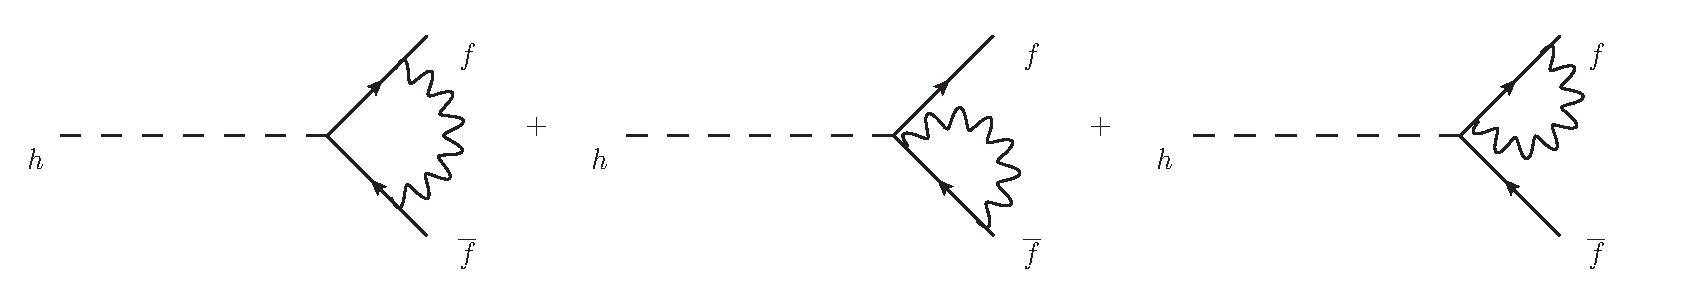
\includegraphics[width=0.7\linewidth]{./figs/yukawa_beta/1.eps}}} \\
   &\SU(2) \times \Uni(1)_\text{Y} \text{ corr. } \vcenter{\hbox{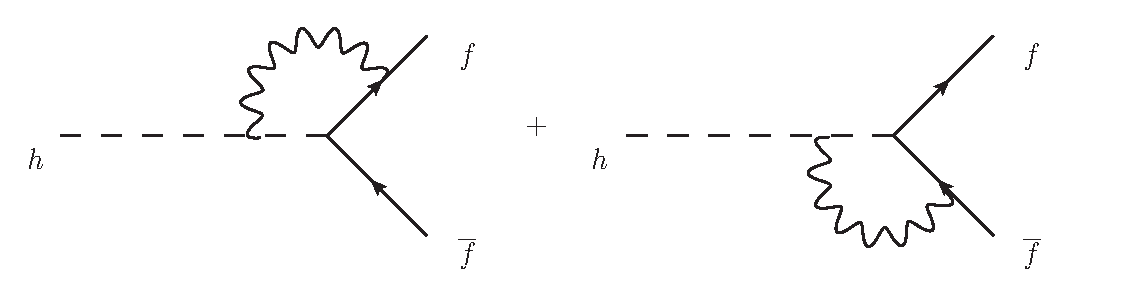
\includegraphics[width=0.5\linewidth]{./figs/yukawa_beta/2.eps}}} \\
   &\text{Yukawa corr. } \vcenter{\hbox{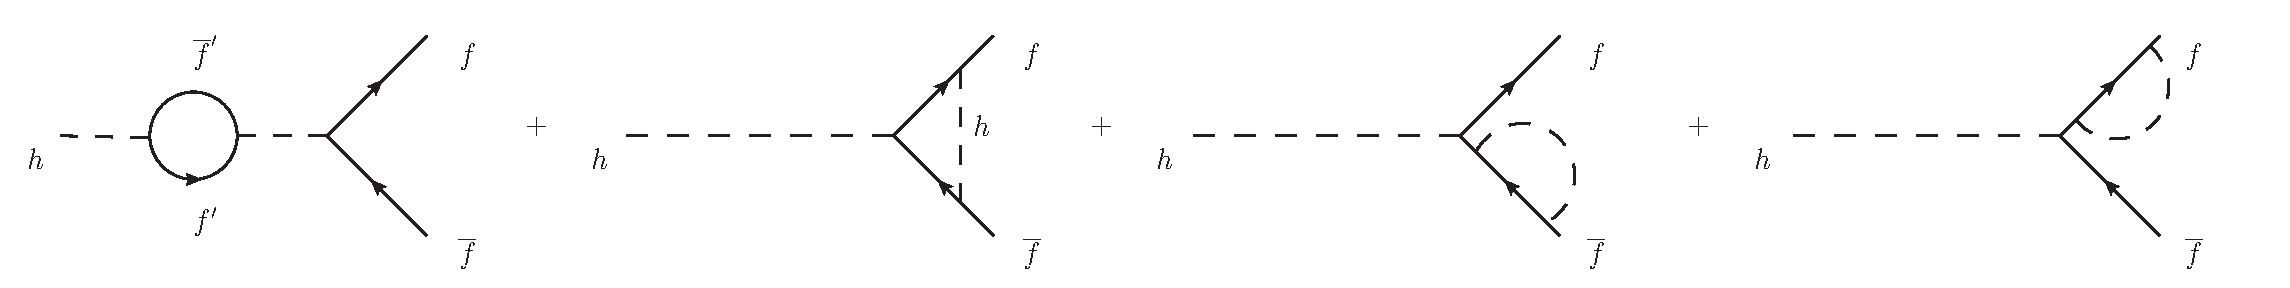
\includegraphics[width=0.95\linewidth]{./figs/yukawa_beta/3.eps}}}
\end{align*}

Couplings to Higgs are ($f=y$)
\begin{align}
   \dv{f_t}{\ln Q} &= \frac{f_t}{16\pi^2} \left[ -3 \left( \frac{8}{3} g_3^2 + \frac{3}{4} g_2^2 + \frac{17}{36} g_Y^2 \right)  + \frac{1}{2} \left( gf_t^2 + 3 f_b^2 + 2f^2_\tau \right) \right] \label{2.43a} \\
   \dv{f_b}{\ln Q} &= \frac{f_b}{16\pi^2} \left[ -3 \left( \frac{8}{3} g_3^2 + \frac{3}{4} g_2^2 + \frac{5}{36}g_Y^2 \right)  + \frac{1}{2} \left( 3 f_t^2 + g f_b^2 + 2f_\tau^2 \right)  \right] \label{2.43b} \\
   \dv{f_\tau}{\ln Q} &=  \frac{f_\tau}{16\pi^2} \left[ -3 \left( \frac{3}{4} g_2^2 + \frac{5}{4} g_Y^2 \right) + \frac{1}{ 2} \left( 6 f_t^2 + 6 f_b^2 + 5 f_\tau^2 \right) \right] \label{2.43c}
\end{align}

They can be solved analytically if Yukawa terms on RHS are neglected
\begin{subequations}
   \label{2.44}
\begin{alignat}{5}
   & f_t(Q) &&= f_t(M_X) \cdot  &&\left[ \frac{\alpha_3 (Q)}{ \alpha_3 (M_X)} \right]^{\frac{4}{b_3}} \cdot &&\left[ \frac{\alpha_2 (Q)}{\alpha_2 (M_X)} \right]^{\frac{g}{8b_2}} \cdot &&\left[ \frac{\alpha_Y (Q)}{\alpha_Y(M_X)} \right]^{\frac{17}{24b_Y}} \label{2.44a}\\
   &f_b(Q) &&= f_b(M_X) \cdot &&\left[ \frac{\alpha_3 (Q)}{\alpha_3 (M_X)} \right]^{\frac{4}{b_3}} \cdot &&\left[ \frac{\alpha_2 (Q)}{\alpha_2(M_X)} \right]^{\frac{g}{8b_2}} \cdot &&\left[ \frac{\alpha_Y (Q)}{\alpha_Y (M_X)} \right]^{\frac{5}{24 b_Y}} \label{2.44b}\\
   &f_\tau (Q) &&= f_\tau (M_X) \cdot &&  && \left[ \frac{\alpha_2(Q)}{\alpha_2(M_X)} \right]^{\frac{g}{8b_2}} \cdot && \left[ \frac{\alpha_Y (Q)}{\alpha_Y(M_X)} \right]^{\frac{15}{8b_Y}} \label{2.44c}
\end{alignat}
\end{subequations}
Details abound the derivation see homework. Note that all three factors in the bracket are larger than $1$. Because $Q < M_x$ and thus $\frac{\alpha_3(Q)}{\alpha_3(M_X)} > 1$ ($4/b_3 > 0$), $\frac{\alpha_2(Q)}{\alpha_2(M_X)} > 1$ ($g/8b_2 > 0$), and $\frac{\alpha_Y(Q)}{\alpha_Y(M_X)} < 1$ ($15/8b_Y < 0$). Thus gauge interactions increase Yukawa couplings when going down in energy!

Yukawa couplings can be ignored when considering ratios of first or second generation fermion masses!
\begin{align}
   \frac{f_s(M_Z)}{f_\mu(M_Z)} &= \frac{f_s(M_X)}{f_\mu (M_X)} \cdot \left[ \frac{\alpha_s(M_Z)}{\alpha_s(M_X)} \right]^{4/7} \cdot \left[ \frac{\alpha_Y(M_Z)}{\alpha_Y(M_X)} \right]^{1/4} \label{2.45}\\
                               &= 1 \cdot 2.7 \cdot 0.9 = 2.4 \label{2.46}
\end{align}
where $f_s(M_X) / f_\mu(M_X) = 1$ in minimal $\SU(5)$. Need $f_s \simeq f_\mu$ at $Q \sim [1,2] \si{\giga\eV}$: (\ref{2.46}) is off by factor $5$. $f_d \simeq 20 f_3$ at $Q \simeq \SI{1}{\giga \eV}$: (\ref{2.46}) is too small by factor $4$.

However, $f_b / f_\tau$ does work more or less! Also $f_t(M_X) < \infty$ gives upper bound on $f_t(m_t)$!

Mixed success of minimal $\SU(5)$. Light fermion masses can be patched up, i.e.~by introducing a Yukawa coupling to $45_H$ or via non-renormalizable operators.

Yukawa interactions (\ref{2.41}) also lead to proton decay through exchange of triplet partner of SM Higgs $h_3$:
\begin{equation}
   \vcenter{\hbox{
         \feynmandiagram[horizontal=v1 to v2]{
            i1[particle=\(d\)] --[fermion] v1 --[anti fermion] i2[particle=\(u\)];
            v1 --[scalar, edge label=\(h_3^*\)] v2;
            f1[particle=\(e\)] --[fermion] v2 --[anti fermion] f2[particle=\(u\)];
         };
   }}: u + d \rightarrow e^+ + \overline{u}
\end{equation}
Need large mass for $h_3$! Simple mass term $m_{H_5}^2 |H_5|^2$ is not sufficient, it would also give positive squared mass $m_{H_5}^2$ to SM Higgs. Then no $\SU(2) \times \Uni(1)_\text{Y}$ breaking!

%%%%% Lecture 9a
We need mass term for $H_5$ that is not $\SU(5)$ invariant. From coupling to $\Sigma$!
\begin{align}
   V(\Sigma, H_5) &= m_H^2 |H_5|^2 + \alpha |H_5|^2 \tr(\Sigma^2) + \beta H_5^\dagger \sigma^2 H_5 \notag \\
                  &\stackrel{\Sigma \rightarrow \expval{\Sigma}}{\longrightarrow} m_H^2 \left( |h|^2 + |\phi|^2 \right) + \alpha \frac{v_x^2}{2} \left( |h|^2 + |\phi|^2 \right) + \beta v_x^2 \left( \frac{1}{15} |h|^2 + \frac{3}{20} |\phi|^2 \right) \label{2.48}
\end{align}
Thus
\begin{align*}
   m_\phi^2 &= m_H^2 + v_x^2 \left( \frac{\alpha}{2} + \frac{3\beta}{20} \right)  \stackrel{!}{=} \order{-M_Z^2}\\
   m_h^2 &= m_H^2 + v_x^2 \left( \frac{\alpha}{2} + \frac{\beta}{15} \right)  \stackrel{!}{=} \order{M_X^2}
\end{align*}
Need $\beta < 0$, and thus delicate cancellation in $m_\phi^2$ to 1 part in $10^{30}$!
\begin{equation}
   m_\phi^2 = m_h^2 + \frac{\beta v_x^2}{12} \stackrel{!}{=} \order{-M_Z^2} \label{2.49}
\end{equation}
From proton decay we must have $m_{h}$ quite large and $v_x$ is roughly the unification scale, but the Higgs mass $m_\phi$ is much lower. This is the \textit{doublet-triplet splitting problem}. Note that even if (\ref{2.49}) is satisfied at tree level, it will be destroyed by loop corrections of order $\frac{\alpha}{\pi} M_X^2$!

Final problem of minimal $\SU(5)$ is there no neutrino masses yet! For renormalizable neutrino masses we need $\nu_R$! Right-handed neutrino is singlet of $\SU(5)$, just added "by hand". If $M_{\nu_R} \sim M_X$, the theory agrees with estimate (\ref{1.61}) in see-saw models roughly. However, in $\SU(5)$, $M_{\nu_R}$ can be anything.

\paragraph{Summary} 

Pro's
\begin{itemize}
   \item explains ordering of gauge couplings
   \item explains quantization of electric charges
   \item get $m_b / m_\tau$ roughly correct (minimal model)
\end{itemize}
Con's
\begin{itemize}
   \item gauge couplings not quite right
   \item if $M_X$ defines via electroweak couplings, protons have too short half life
   \item still need several representations for one generations of SM matter field $10 + \overline{5} (+1)$ ($1$ for right-handed neutrino)
   \item Doublet-triplet splitting requires extreme fine-tuning
\end{itemize}

\section{$\SO(10)$ Unification} 
It solves the third problem!

$\SO(10)$ is the special orthogonal group, rotations in $10$ Euclidean dimensions. Generators are anti-symmetric real $10\times 10$ matrices: $\underline{45}$ is adjoint representation of $\SO(10)$.

$\SO(10)$ has rank $5$, one extra diagonal generator beyond SM.

Decomposition under $\SU(5)$ multiplets
\begin{equation}
   \underline{45} = 24 + 10 + \overline{10} + 1 \label{2.51}
\end{equation}
The extra $\Uni(1)$ generator: gauged $B$-$L$ symmetry!

Whole SM generation fits into $16$-dimensional ("spinor") representation of $\SO(10)$
\begin{equation}
   16  = 10 + \overline{5} + 1 \label{2.51} 
\end{equation}
The $1$ corresponds to $\nu_R$.

SM Higgs fits in fundamental $10$-dimensional representation
\begin{equation}
   10 = 5 + \overline{5} \label{2.52}
\end{equation}
There are two scalar doublets!

Simplest fermion mass term: $16\times 16 \times 10$
\begin{align}
   m_\tau = m_b \quad m_{\nu_R} = m_t \label{2.52}
\end{align}
at unification scale with $m_{\nu}$ Dirac mass. Note that $\nu_R$ is not singlet of $\SO(10)$, then it gets its (large) mass from Higgs mechanism, e.g.~from 126 (1): need to break $B$-$L$. $\SO(10)$ allows several symmetry breaking chains
\begin{equation}
   \SO(10) \stackrel{45}{\longrightarrow} \SU(5) \times \Uni(1)' \stackrel{126}{\longrightarrow} \SU(3) \times \SU(2) \times \Uni(1)_\text{Y} \label{2.53}
\end{equation}
Note that the $\SU(5)$ can be "flipped" $\SU(5)$ with $u^c \in \overline{5}$, $\Uni(1)_\text{Y}$ is combination of $\Uni(1)'$ and $t_{12}$ and $126$ contains $M_{\nu_R}$ generator.

Or
\begin{equation}
   \SO(10) \stackrel{16}{\longrightarrow} \SU(5) \stackrel{45}{\longrightarrow} \SU(3) \times \SU(2) \times \Uni(1)_\text{Y} \label{2.54}
\end{equation}
Or
\begin{equation}
   \SO(10) \stackrel{54}{\longrightarrow} \SU(4) \times \SU(2)_\text{L} \times \SU(2)_\text{R} \stackrel{45}{\longrightarrow} \SU(3) \times \SU(2)_\text{L}\times \SU(2)_\text{R} \times \Uni(1)_\text{B-L} \stackrel{16}{\longrightarrow} \SU(3) \times \SU(2) \times \Uni(1)_\text{Y} \label{2.55}
\end{equation}
(Pati and Salam, 1974). It has intermediate scales, which can be adjusted to obtain exact gauge coupling unification, thus no prediction!

Last step of symmetry breaking might be at relatively low scale, it might have extra gauge gauge bosons, from $\SU(2)_\text{R} \times \Uni(1)_{B-L}$ at accessible energies!

Note that every representation of $\SO(10)$ is anomaly-free! (Not true in $\SU(5)$)

\section{Non-Renormalizable Operators}
GUT scale is not too far from (reduced) Planck scale, $M_p = \SI{2.4e18}{\giga \eV}$ ($G_N = \frac{1}{8\pi M_p^2}$).

Non-Renormalizable operators suppresses by inverse powers of $M_p$ may be important! Such operators are "generically" expected to occur in theories including gravity (supergravity, superstrings), unless forbidden by some symmetry of the full theory.

\paragraph{Example 1} Modification of gauge coupling unification! In renormalizable Yang-Mills theory, the gauge kinetic term
\begin{equation}
   \lag_{\text{g}-\text{k}} = - \frac{1}{4} F^a_{\mu\nu} F^{\mu \nu a} = - \frac{1}{2} \tr (F_{\mu\nu}F^{\mu\nu})  \label{2.56}
\end{equation}
with 
\begin{equation}
   F_{\mu\nu} = \sum_{a} t^a F^a_{\mu\nu}  \label{2.57}
\end{equation}
and $\tr(t^a t^b) = \frac{1}{2} \delta^{ab} $.

In case of $\SU(5)$, from (\ref{2.12})
\begin{equation}
   F_{\mu\nu} = \begin{pmatrix} G_{\mu\nu} + \frac{1}{\sqrt{15}} B_{\mu\nu} \cdot \id_{3} & X^-_{\mu\nu} \\ X^\dagger_{\mu\nu} & W_{\mu\nu} - \frac{3}{2\sqrt{15}}B_{\mu\nu} \id_2  \end{pmatrix} \label{2.58}
\end{equation}
with $G_{\mu\nu}$ gluon field, $X$ gauge field for $X^-$, $Y$ bosons and $W_{\mu\nu}$ for $W$ bosons.


Including a non-renormalizable term, \eqref{2.56} extends to 
\begin{equation}
   \lag_{g-k} = -\frac{1}{2} \tr(F^{\mu\nu}F_{\mu\nu}) - \frac{\kappa}{2M_p} \tr(F_{\mu\nu} \Sigma F^{\mu\nu}) + \order{M_P^{-2}} \label{2.59}
\end{equation}
with $\Sigma$ $\underline{24}$ of $\SU(5)$.

(\ref{2.31}) and (\ref{2.58})
\begin{align*}
   \expval{\Sigma} F_{\mu\nu} &= \frac{v_x}{2\sqrt{15}} \begin{pmatrix} 2 G_{\mu\nu} + \frac{2}{\sqrt{15}}B_{\mu\nu} \id_3 & 2X^-_{\mu\nu} \\ -3X^\dagger_{\mu\nu} & -3 W_{\mu\nu} + \frac{9}{2\sqrt{15}}B_\mu \id_2 \end{pmatrix} \\
   \tr_{\SU(5)}(F_{\mu\nu} \Sigma F^{\mu\nu}) &= \frac{v_x}{2\sqrt{15}} \left[ 2 \tr_{\SU(3)} (G_{\mu\nu}G^{\mu\nu}) - 3 \tr_{\SU(2)} (W_{\mu\nu}W^{\mu\nu}) - \frac{1}{2} B_{\mu\nu} B^{\mu\nu} + \dots  \right]
\end{align*}
(\ref{2.59}) gives for SM gauge bosons
\begin{equation}
   \lag^\text{SM}_{g-k} = -\frac{1}{2} \tr(G_{\mu\nu}G^{\mu\nu}) \left[ 1 + \frac{\kappa v_x}{\sqrt{15} M_p} \right] - \frac{1}{2} \tr(W_{\mu\nu}W^{\mu\nu}) \left[ 1 - \frac{3\kappa v_x}{2\sqrt{15}M_p} \right] - \frac{1}{4} B_{\mu\nu} B^{\mu\nu} \left[ 1 - \frac{\kappa v_x}{\sqrt{15} M_p} \right] + \order{M_p^{-2}} \label{2.60}
\end{equation}

To get standard form of bilinear terms, we have to re-scale fields
\begin{align}
   \begin{split}
      A_\mu^a &\rightarrow \frac{1}{\sqrt{1+ r}} A^a_\mu  \\
      W^i_\mu &\rightarrow \frac{1}{\sqrt{1-3r/2}} W_\mu^i  \\
      B_\mu &\rightarrow \frac{1}{\sqrt{1 - r}} B_\mu  \\
      r &= \frac{\kappa v_x}{\sqrt{15} M_p}
   \end{split}\label{2.61}
\end{align}
In rest of Lagrangian, gauge field always comes multiplied with gauge coupling: (\ref{2.61}) is equivalent to re-scaling of the gauge couplings!
\begin{equation}
   g_3 \rightarrow \frac{1}{\sqrt{1+r}} g_3, \quad g_2 \rightarrow \frac{1}{\sqrt{1-3r/2}} g_2, \quad g_Y \rightarrow \frac{1}{\sqrt{1-r}} g_Y
\end{equation}
This is true at scale $M_X$. After re-scaling, gauge couplings no longer unify! If terms $\order{M_P^{-2}}$are included, we can achieve unification of gauge couplings at any scale of order Planck scale, with any value of GUT gauge coupling!

\paragraph{Example 2} Froggat-Neilsen Mechanism

In order to explain hierarchy of Yukawa couplings, to introduce flavor symmetry. Simplest possibility would be $\Uni(1)_F$.

Flavor symmetry is broken by "flavon" field $f$, which is a singlet under $\SU(5)$.

Introduce small parameter 
\begin{equation}
   \epsilon = \frac{\expval{f}}{M_p} < 1 \label{2.63}
\end{equation}

Assign $U(1)_F$ charges: e.g.
\begin{align}
   \begin{split}
   F(f) &= 1, \\
   F(H_5) &= F(\psi_3) = F(\chi_3) = 0, \\
   F(\psi_2) &= F(\chi_2) = -1, \\
   F(\psi_1) &= F(\chi_1) = -2 \label{2.64}
   \end{split}
\end{align}
with
\begin{align*}
   \psi_3 &= (b^c, \tau, \nu_\tau), 
          &&\chi_3 = (b, t, \tau^c) \\
   \psi_2 &= (s^c, \mu, \nu_\mu ),
          && \chi_2 = (c,s,\mu^c) \\
   \psi_1 &= (d^c, e, \nu_e),
          && \chi_1 = (u, d, e^c)
\end{align*}

Yukawa couplings (\ref{2.41}) only allowed for third generation fermions! More generally:
\begin{equation}
   \lag_\text{Yuk}^\text{eff} = \sum_{i,j} \left[ \lambda_{ij}^d \epsilon^{|F(\psi_1) + F(\chi_j)|}  \overline{\psi^c_i} \chi_j H_5^\dagger -  \frac{\lambda_{ij}^u}{4} \epsilon^{|F(\chi_i)+F(\chi_j)|}\overline{\chi^c_i} \chi_j H_5 + h.c. \right] \label{2.65}
\end{equation}
This can lead to (semi-)realistic quark and lepton mass matrices with all $\lambda^d_{ij}, \lambda^u_{ij} \sim \order{1}$ with 
\begin{equation}
   \epsilon \sim \theta_c \cong \frac{1}{5} \label{2.66}
\end{equation}

We can get structure like (\ref{2.65}) also in a renormalizable theory, by integrating out heavy fermions. E.g.
\begin{align*}
\begin{tikzpicture}   
\begin{feynman}
   \vertex (i) {\(\psi_R\)};
   \vertex[right=2cm of i] (v1);
   \vertex[right=2cm of v1] (v2);
   \vertex[right=2cm of v2] (f) {\(\psi_L\)};
   \vertex[above=2cm of v1] (m1) {\(\expval{f}\)};
   \vertex[above=2cm of v2] (m2) {\(\expval{\phi}\)};
   \diagram*{
      (i) -- (v1) --[insertion=0.5, edge label={\(F_L, F_R\)}] (v2) -- (f),
      (m1) --[scalar] (v1),
      (m2) --[scalar] (v2),
   };
\end{feynman}
\end{tikzpicture}
\end{align*}
gives $\epsilon = \expval{f} / m_F$ suppression.

Symmetry must allow bare $\overline{F_L} F_R$ mass term: $F_{L,R}$ are in vector-like representation of gauge group. Symmetry must allow $\psi_R F_L f$ and $F_R \psi_L \phi$ couplings, but must forbid $\overline{\psi}_R \psi_L H$. Similar to see-saw!

\chapter{Supersymmetry}
\section{The hierarchy problem and its SUSY solution}

Problem is that scalar (Higgs) section of the SM is not stable against radiative corrections!

\paragraph{Two point function of electron} (related to electron mass): a well-behaved example
\begin{align}
   &\feynmandiagram[horizontal=a to v1, layered layout]{
      a[particle=\(e\)] --[fermion, momentum'=\(q\)] v1 --[fermion, momentum'=\(k\)] v2 --[fermion, momentum'=\(q\)] b[particle=\(e\)],
      v1 --[half left, photon, momentum={\(q-k\)}] v2,
   }; \notag \\
   \pi^{ee}(q\rightarrow 0) &=  \int \frac{\dd[4]{k}}{(2\pi)^4} (ie\gamma_\mu) \frac{-i g^{\mu\nu}}{k^2} \frac{i}{\slashed{k}-m_e} (ie \gamma_\nu) \notag \\
                            &= - e^2 \int \frac{\dd[4]{k}}{(2\pi)^4} \frac{1}{k^2 (k^2 - m_e^2)} \gamma_\mu (\slashed{k} + m_e )\gamma^\mu \notag \\
                            &= -e^2 m_e \int \frac{\dd[4]{l}}{(2\pi)^4} \frac{\gamma_\mu \gamma^\mu}{k^2 (k^2 - m_e^2)} \label{3.2}
\end{align}

Note
\begin{itemize}
   \item Correction vanished if tree-level $m_e \rightarrow 0$
   \item Correction "only" diverge logarithmically
      \begin{equation}
         \delta m_e \sim m_e \frac{\alpha}{\pi} \ln \frac{\Lambda}{m_e}  \label{3.3}
      \end{equation}
      with $\Lambda$ a cut-off parameter, e.g.~take $\Lambda = M_{pl} = \SI{2.4e18}{\giga\eV} = \num{4.7e21} \cdot m_e$
      \begin{equation}
         \delta m_e \cong \frac{m_e}{8}
      \end{equation}
\end{itemize}

Small electron mass remains small! Reason for this is that setting $m_e \rightarrow 0$ increases the symmetry of the theory. Lagrangian becomes invariant under global chiral $\Uni (1)$ transformation
\begin{equation}
   \psi \rightarrow e^{i \chi \gamma_5 } \psi = (\cos \chi + i \gamma_5 \sin \chi) \psi
\end{equation}
with $\chi = \text{const.}$. The bilinear $\overline{\psi} \gamma_\mu \psi$ is invariant under this transformation
\begin{align}
   \overline{\psi} \gamma_\mu \psi &\rightarrow \overline{\psi} (\cos \chi - i \overline{\gamma}_5 \sin \chi) \gamma_\mu (\cos \chi + i \gamma_5 \sin \chi) \psi \notag \\
                                   &= \overline{\psi} (\cos \chi + i \gamma_5 \sin \chi) (\cos \chi - i \gamma_5 \sin \chi) \gamma_\mu \psi \notag \\
                                   &= \overline{\psi} ((\cos \chi)^2 - (i \gamma_5 \sin \chi)^2) \gamma_\mu \psi = \overline{\psi} \gamma_\mu \psi \label{3.6}
\end{align}
But $\overline{\psi} \psi$ not
\begin{equation}
   \overline{\psi} \psi \rightarrow \overline{\psi} (\cos \chi  i \gamma_5 \sin \chi)^2 \psi \neq \overline{\psi} \psi \label{3.7}
\end{equation}
Fermion masses or Yukawa couplings break chiral symmetry. Conversely, $f^{(e)}\rightarrow 0$ restores chiral symmetry.

Small fermion mass is technically natural (t' Hooft), as it will remain small in all orders in perturbation theory!

\paragraph{Two-point function of Higgs boson}
\begin{align}
   &\feynmandiagram[horizontal=i to v1, layered layout]{
      i[particle=\(h\)] --[scalar] v1 --[half left, fermion, edge label=\(t\)] v2 --[scalar] f[particle=\(h\)],
      v2 --[half left, fermion, edge label=\(t\)] v1,
   }; \notag \\
   \Pi^h_t (0) &= - 3 \int \frac{\dd[4]{k}}{(2\pi)^4} \tr[ - i \frac{f^{(t)}}{\sqrt{2}} \frac{i}{\slashed{k} - m_t} \left( -i \frac{f^{(t)}}{\sqrt{2}} \right) \frac{i}{\slashed{k} - m_t} ] \notag \\
               &= -\frac{3}{2} f^{(t) \, 2} \int \frac{\dd[4]{k}}{(2\pi)^4} \frac{1}{(k^2 - m_t^2)^2 } \tr[ (\slashed{k} + m_t) (\slashed{k} + m_t)] \notag \\
               &= -6 f^{(t) \, 2} \int \frac{\dd[4]{k}}{(2\pi)^4} \frac{k^2 + m_t^2}{(k^2 - m_t^2)^2} \label{3.5}
\end{align}
where negative sign comes from closed fermion loop and $3$ from colors.

Note
\begin{itemize}
   \item Result diverges quadratically!
   \item Correction does not depend on tree-level Higgs mass
      \begin{equation}
         \delta m_h^2 \sim \frac{3 f{(t)\, 2}}{8\pi^2 } \Lambda^2 \label{3.6}
      \end{equation}
\end{itemize}
For $\Lambda=M_{pl}$: 
\begin{equation}
   \delta m_h^2 \sim \num{1e30} m^2_{h, \text{phys}}  \label{3.7}
\end{equation}
Since 
\begin{equation}
   m^2_{h, \text{phys}} = m^2_{h,0} + \delta m^2_h \label{3.8}
\end{equation}
it needs cancellation to $1$ part in $10^{30}$. This extreme \textit{finetuning} is not \textit{natural}. Reason is that $m_h \rightarrow 0$ does not increase symmetry of SM (at quantum level). Following t' Hooft, Susskind, Weinberg: $m_h$ should be close to highest scale when SM is applicable! If there exists physical scale $M \gg m_h$, we expect finite corrections $\sim \alpha/\pi M^2$!

\paragraph{Example} for a successful cure of a finetuning problem

In standard cosmology, the energy density of the Universe in units of the critical energy density $\Omega = \rho / \rho_\text{crit}$ is time-dependent.
\begin{equation*}
   \Omega(t) - 1 \sim \left[ \Omega(t_0) - 1 \right] \cdot \left[ \frac{T(t_0)}{T(t)} \right]^{\beta}
\end{equation*}
with $\beta=1$ or $2$.

Now $\Omega(t_0) = 1.00 \pm 0.03$. If $ T \gg T_0 (\sim \SI{1e-4}{\eV})$
\begin{equation*}
   |\Omega(t_0) -1 | \gg |\Omega(t) - 1|
\end{equation*}
Need $|\Omega(t) - 1| \gg 1$ at $T \gg T_0$: fine-tuning of initial conditions!

This fine-tuning is solved by postulating very early epoch of exponential growth called "inflation"! Generically predicts $|\Omega(t_0) - 1| \ll 1$. Predictions for fluctuations in CMB have been confirmed! Nature really abhors finetuning (?).

Counter-example is the potential equivalence of vacuum energy and cosmological constant. Naively it corresponds to zero-point function, which has a quartic divergence in field theory (mode sum, $\sim \int \frac{\dd[4]{k}}{(2\pi)^4}$). It gets reduced to quadratic divergence in softly broken SUSY. There is no (convincing) solution known. We may need theory of quantum gravity. 

Back to (\ref{3.6}), (\ref{3.8}): Absence of serious finetuning, i.e.~
\begin{equation}
   \delta e_h^2 \lessapprox m_{h, \text{phys}}^2
   \label{3.9}
\end{equation}
implies
\begin{equation}
   \Lambda \lessapprox \order{1} \si{\tera \eV}
   \label{3.10}
\end{equation}
SM must be replaced by a different theory at (few) $\si{\tera\eV}$ scale!

One possibility is that SM to theory without elementary scalars, i.e.~$h$ is composite. This is the idea behind technicolor theories. It has following problems
\begin{itemize}
   \item "New physics" is not sufficiently decoupling. It generically expects sizeable effects in precision experiments and they have not been seen.
   \item Higgs mechanism also responsible for fermion masses in SM. It becomes difficult to generate a large top mass without generating much too large FCNC!
   \item New interactions need to be very strongly coupled, thus difficult to perform reliable calculations.
\end{itemize}
People keep trying but there is no convincing solution known.

Here we consider second option, supersymmetry: quadratic divergences cancel order by order. To this end, we need superpartners for each SM particle, with "same" interactions, but spin differing by $1/2$ unit.

Here to consider "stops" $\SU(2)_L$ doublet $\tilde t_L$, and singlet $\tilde t_R$. They both are complex scalars and color triplets.
\begin{equation}
   \lag_{\tilde t h} = \tilde \lambda_t |\phi^0|^2 \left( |\tilde t_L|^2 + |\tilde t_R|^2 \right) + \left[ f^{(t)} A_t \phi^0 \tilde t_L \tilde t_R^* + h.c. \right]
   \label{3.11}
\end{equation}
It gives new diagrams
\begin{equation*}
   \begin{tikzpicture}[scale=1, transform shape, baseline=(i.base)]
      \begin{feynman}
         \vertex (i) {\(h\)};
         \vertex[right=1.5cm of i, label=270:{\(i\tilde \lambda_t\)}, dot] (v) ;
         \vertex[above=1.5cm of v, label=90:{\(\tilde t_{L,R}\)}] (x) ;
         \vertex[right=1.5cm of v] (f) {\(h\)};
         \diagram*{
            (i) --[scalar] (v) --[scalar] (f),
            (v) --[scalar, half left] (x) --[scalar, half left] (v),
         };
      \end{feynman}
   \end{tikzpicture}
   +    
   \begin{tikzpicture}[scale=1, transform shape, baseline=(i.base)]
      \begin{feynman}
         \vertex (i) {\(h\)};
         \vertex[right=1.5cm of i, label=235:{\(i\sqrt{2}\tilde \lambda_t v\)}] (v1) ;
         \vertex[right=1.5cm of v1] (v2) ;
         \vertex[right=1.5cm of v2] (f) {\(h\)};
         \diagram*{
            (i) --[scalar] (v1)[dot] --[scalar, half left, edge label={\(\tilde t_{L,R}\)}] (v2) --[scalar] (f),
            (v1) --[scalar, half right, edge label'={\(\tilde t_{L,R}\)}] (v2),
         };
      \end{feynman}
   \end{tikzpicture}
   +
   \begin{tikzpicture}[scale=1, transform shape, baseline=(i.base)]
      \begin{feynman}
         \vertex (i) {\(h\)};
         \vertex[right=1.5cm of i, label=235:{\(f^{(t)}A_t/\sqrt{2}\)}] (v1) ;
         \vertex[right=1.5cm of v1] (v2) ;
         \vertex[right=1.5cm of v2] (f) {\(h\)};
         \diagram*{
            (i) --[scalar] (v1)[dot] --[scalar, half left, edge label={\(\tilde t_{L,R}\)}] (v2) --[scalar] (f),
            (v1) --[scalar, half right, edge label'={\(\tilde t_{R,L}\)}] (v2),
         };
      \end{feynman}
   \end{tikzpicture}
\end{equation*}
\begin{align}
   \Pi^h_{\tilde t} (0) &= 3 \int \frac{\dd[4]{k}}{(2\pi)^4} \Bigg[ i \tilde \lambda_t \left( \frac{i}{k^2 - m^2_{\tilde{t}_L}} + \frac{i}{k^2 - m^2_{\tilde t_R}} \right) 
                         + (i\sqrt{2} \tilde \lambda_t v)^2 \left( \frac{i^2}{(k^2 - m^2_{\tilde t_L})^2} + \frac{i^2}{(k^2 - m^2_{\tilde t_R})^2} \right) \notag \\
                        &\quad + 2 \left( \frac{if^{(t)} A_t}{\sqrt{2}} \right)^2 \frac{i^2}{(k^2 - m^2_{\tilde t_L})(k^2 - m^2_{t_R})} \Bigg] \notag \\
                        &= 3 \int \frac{\dd[4]{k}}{(2\pi)^4} \Bigg[ - \tilde \lambda_{t} \left( \frac{1}{k^2 - m^2_{\tilde t_L}} + \frac{1}{k^2 - m^2_{\tilde t_R}} \right) 
                         + 2 (\tilde{\lambda}_t v)^2 \left( \frac{1}{(k^2 - m^2_{\tilde{t}_L})^2} + \frac{1}{(k^2 - m^2_{\tilde{t}_R})^2} \right) \notag \\
                        &\quad + \left(f^{(t)} A_t\right)^2 \frac{1}{(k^2 - m^2_{\tilde t_L})(k^2 - m^2_{\tilde t_R})} \Bigg] \label{3.12}
\end{align}
Only first term in (\ref{3.12}) has quadratic divergence.

The quadratic divergence gets cancelled from (\ref{3.5}) if
\begin{equation}
   \tilde \lambda_t = - f^{(t)2}
   \label{3.13}
\end{equation}
Note that $\tilde \lambda_t < 0$ for potential to be bounded from below!
\begin{align}
   \Pi_{t + \tilde{t}}^h(0) &= 3 f^{(t)2} \cdot \int \frac{\dd[4]{k}}{(2\pi)^4} \Bigg[ -2 \frac{k^2 + m_t^2}{(k^2 - m^2_t)^2} + \frac{1}{k^2 - m_{\tilde t_L}^2} + \frac{1}{k^2 - m^2_{\tilde t_R}} + 2 (f^{(t)}v)^2 \left( \frac{1}{(k^2 - m_{\tilde t_L})^2} + \frac{1}{(k^2 - m^2_{\tilde t_R})^2} \right) \notag \\
                            &\quad+ A^2_t \frac{1}{(k^2 - m_{\tilde t_L}^2)(k^2 - m^2_{\tilde t_R})} \Bigg] \notag \\
                            &=3 f^{(t)2} \int \frac{\dd[4]{k}}{(2\pi)^4} \Bigg[ \frac{m^2_{\tilde t_L} - m^2_t}{(k^2 - m_t^2)(k^2 - m^2_{\tilde t_L})} + \frac{m^2_{\tilde t_R}-m^2_t}{(k^2 - m_t^2)(k^2 - m^2_{\tilde t_R})} + 2m^2_t \left( \frac{1}{(k^2 - m^2_{\tilde t_L})^2} + \frac{1}{(k^2 - m^2_{\tilde t_R})^2} - \frac{2}{(k^2 - m^2_t)^2} \right)\notag \\
                            &\quad + A^2_t \frac{1}{(k^2 - m^2_{\tilde t_L})(k^2 - m^2_{\tilde t_R})} \Bigg] \label{3.14} 
\end{align}

Note that 
\begin{itemize}
   \item equation (\ref{3.14}) is only logarithmically divergent!
   \item if 
      \begin{align}
         m_t &= m_{\tilde t_L} = m_{\tilde t_R} \label{3.15a}\\
         A_t &= 0 \label{3.15b}
      \end{align}
      then
      \begin{equation}
         \pi^h_{t + \tilde{t}}(0) =0 \label{3.16}
      \end{equation}
\end{itemize}
More generally
\begin{equation}
   \delta m_h^2 \sim \frac{3 f^{(t)2}}{8\pi^2} \cdot \ln \frac{\Lambda}{m_n} \cdot [(m^2_{\tilde t} - m^2_t), A^2_t] \label{3.17}
\end{equation}
So we want $m_{\tilde{t}}, |A_t| \lessapprox \order{1}\si{\tera \eV}$!

In order to enforce cancellation of quadratic divergence in all orders of perturbation theory, and for all interactions, we need to supersymmetrize the entire SM, i.e.~we need a superpartner for each SM particle: doubling of particle spectrum!

Recall that chiral symmetry also double fermion spectrum! It is also helpful to remove divergences.

In classical EM, non-relativistic QM: $\delta m_e \sim e^2 \cdot \Lambda$. In QFT, this becomes a logarithmic divergence, but needs positrons!

\section{Grassmann variables}
SUSY connects (commuting) bosons with (anti-commuting) fermions. Most elegant "superfield" formalism is based on "supersymmetrization of space-time". To that end, introduce anti-commuting "Grassmann" coordinates.

For one complex $\theta$, with conjugate $\bar{\theta}$ ($\bar{\bar{\theta}}=\theta$), we postulate
\begin{subequations}
   \label{3.18}
\begin{align}
   \acomm{\theta}{\theta} &= \acomm{\bar\theta}{\bar\theta} = 0 \label{3.18a}\\
   \acomm{\theta}{\bar\theta} &= 0 \label{3.18b}
\end{align}
\end{subequations}
These two relations generate the Grassmann algebra. From them,
\begin{subequations}
\label{3.19}
\begin{align}
   \theta^2 &= \bar{\theta}^2 = 0 \label{3.19a} \\
   \theta \bar\theta &= - \bar \theta \theta \label{3.19b}
\end{align}
\end{subequations}
With (\ref{3.19}), we can exactly expand an analytic function
\begin{equation}
   f(\theta) = f_0 + f_1 \theta \label{3.20}
\end{equation}
with $f_0, f_1 \in \Co$.

Define derivative
\begin{equation}
   \dv{\theta} f(\theta) = f_1 \label{3.21}
\end{equation}
and $\theta f(\theta) = \theta f_0$. 

Equation (\ref{3.20}), (\ref{3.21}) also hold with $\theta \rightarrow \bar \theta$ with $f_0 \rightarrow \bar{f}_0, f_1 \rightarrow \bar{f}_1$. General function
\begin{equation}
   f(\theta, \bar\theta) = f_0 + f_1 \theta + f_2 \bar\theta + f_3 \theta \bar\theta \label{3.22}
\end{equation}
with $\pdv{\theta} f = f_1 + f_3 \bar\theta$, etc..

Integration rules
\begin{subequations}
   \label{3.23}   
\begin{align}
   \int \dd{\theta} \theta &= \int \dd{\bar\theta} \bar{\theta} = 1 \label{3.23a} \\
   \int \dd{\theta} &= \int \dd{\bar\theta} = \int \dd{\theta} \pdv{\theta} f(\theta,\bar\theta) = \int \dd{\bar\theta} \pdv{\theta} f(\theta,\bar\theta) = 0 \label{3.23c} \\
   \int \dd{\theta} \dd{\bar\theta} f(\theta, \bar\theta) &= f_3 \label{3.23b}
\end{align}
\end{subequations}

Integral over Grassmann number is linear
\begin{equation}
   \int \dd{\theta} \left[ \alpha f(\theta) + \beta g(\theta) \right] = \alpha \int \dd{\theta} f(\theta) + \beta \int \dd{\theta} g(\theta) \label{3.24}
\end{equation}

It has translational invariance
\begin{equation*}
   \int \dd{\theta_i} f(\theta_i + \theta_k) = \int \dd{\theta_i} f(\theta_i)
\end{equation*}
independent of $\theta_k$, if $\int \dd{\theta_i} \theta_k = \delta_{ik}$.

Grassmann $\delta$-functions
\begin{subequations}
\label{3.26}   
\begin{align}
   \int \dd{\theta} \delta(\theta) f(\theta) \stackrel{(\ref{3.20})}{=} f_0  \label{3.26a}\\
   \int \dd{\theta} \delta(\theta - \theta') f(\theta) = f(\theta')  \label{3.26b}
\end{align}
\end{subequations}
$\delta$-function has the explicit representation
\begin{equation}
   \delta(\theta - \theta') = \theta - \theta' \label{3.27}
\end{equation}
i.e.~$\delta(\theta) = \theta$.
(\ref{3.26a}) follows from (\ref{3.23a}) and (\ref{3.23c})
\begin{align*}
   \int \dd{\theta} (\theta - \theta') (f_0 + f_1 \theta) &= \int \dd{\theta} \theta f_0 + \int \dd{\theta} \theta f_1 \theta - \int \dd{\theta} \theta' f_0 - \int \dd{\theta} \theta' f_1 \theta  \\
                                                          &= f_0 + 0 + 0 + f_1\theta' \\
                                                          &= f(\theta')
\end{align*}
\section{Algebraic aspects: SUSY algebra and supermultiplets}
Supersymmetry must be spacetime symmetry (like Lorentz symmetry), not internal symmetry (like Yang-Mills gauge symmetry). To see this, consider $2\pi$ rotation operator $U_{2\pi}$ with
\begin{subequations}
   \label{3.28}
\begin{align}
   U_{2\pi} \ket{\text{boson}} &= \ket{\text{boson}} \label{3.28a} \\
   U_{2\pi} \ket{\text{fermion}} &= -\ket{\text{fermion}} \label{3.28b}
\end{align}
\end{subequations}
Supercharge $Q$ transforms bosons into fermions and vice versa
\begin{subequations}
   \label{3.29}
\begin{align}
   Q \ket{\text{boson}} &= \ket{\text{fermion}} \label{3.29a} \\
   Q \ket{\text{fermion}} &= \ket{\text{boson}} \label{3.29b}
\end{align}
\end{subequations}


Then
\begin{align*}
   U_{2\pi} Q U^{-1}_{2\pi} \ket{\text{fermion}} & \stackrel{(\ref{3.28b})}{=} - U_{2\pi} Q U^{-1}_{2\pi} U_{2\pi} \ket{\text{fermion}} \\
                                                 &= - U_{2\pi} Q \ket{\text{fermion}} \\
                                                 &\stackrel{(\ref{3.29b})}{=} - U_{2\pi} \ket{\text{boson}} \\
                                                 & \stackrel{(\ref{3.28a})}{=} - \ket{\text{boson}} \stackrel{(\ref{3.29b})}{=} - Q \ket{\text{fermion}}
\end{align*}
Thus $U_{2\pi} Q U^{-1}_{2\pi} = - Q$, it ($Q$) behaves like spinorial operator. We will need to expand Poincaré algebra to include anti-commutator!

Inhomogeneous Lorentz transformation (Poincaré)
\begin{equation}
   x^\mu \rightarrow x'^{\mu}  = (\delta^\mu_\nu + \omega^\mu_\nu) x^\nu + a^\mu \label{3.30}
\end{equation}
with $\omega_{\mu\nu} = - \omega_{\nu\mu}$. The corresponding unitary operator $U(a) = e^{i a\cdot \underline{P}}$
\begin{equation}
   U(\Lambda) = \exp(- \frac{i}{2} \omega_{\mu\nu} M^{\mu\nu}) \label{3.31}
\end{equation}

Poincaré algebra
\begin{subequations}
   \label{3.32}
\begin{align}
   \comm{\underline{P}_\mu}{\underline{P}_\nu} &= 0 \label{3.32a} \\
   \comm{M_{\mu\nu}}{\underline{P}_\rho} &= i (g_{\nu\rho} \underline{P}_\mu - g_{\mu\rho} P_\nu) \label{3.32b} \\
   \comm{M_{\mu\nu}}{M_{\rho\sigma}} &= -i (g_{\mu\sigma}M_{\nu\rho} - g_{\nu\sigma} M_{\mu\rho} - g_{\nu\rho} M_{\mu\sigma} + g_{\mu\rho} M_{\nu\sigma}) \label{3.32c}
\end{align}
\end{subequations}

Explicit spinorial realization
\begin{equation}
   \Sigma_{\mu\nu} = \frac{i}{4} \comm{\gamma_\mu}{\gamma_\nu}
\end{equation}
thus
\begin{equation}
   M_{\mu\nu} = - x_\mu \underline{P}_\nu + x_\nu \underline{P}_\mu + \Sigma_{\mu\nu} \label{3.35}
\end{equation}

Physically $P_\mu$ is the $4$-momentum and $M_{\mu\nu}$ the total angular momentum, and $\Sigma_{\mu\nu}$ is the spin contribution.

In chiral (Weyl) representation (\ref{0.5})
\begin{equation}
   \Sigma_{\mu\nu} = \begin{pmatrix} \sigma^{\mu\nu} & 0 \\ 0 & \bar{\sigma}_{\mu\nu}\end{pmatrix} \label{3.36a}
\end{equation}
with
\begin{align}
   \sigma^{\mu\nu} &= \frac{i}{4} \left( \sigma^\mu \bar\sigma^\nu - \sigma^\nu \bar \sigma^\mu \right) \label{3.36b} \\
   \bar\sigma^{\mu\nu} &= \frac{i}{4} \left( \bar\sigma^\mu \sigma^\nu - \bar\sigma^\nu \sigma^\mu \right) \label{3.36c}
\end{align}
where
\begin{equation}
   \sigma^\mu = (\id_{2}, \pmb{\sigma}); \quad \bar\sigma^{\mu} = (\id_{2}, - \pmb{\sigma}) \label{3.37}
\end{equation}
and
\begin{equation}
   \bar\sigma^{\mu\nu} = \sigma^{\mu\nu\dagger}
\end{equation}

They have the following properties
\begin{subequations}
\begin{align}
   \acomm{\sigma^\mu}{\bar\sigma^\nu} &= \acomm{\bar\sigma^\mu}{\sigma^\nu} = 2g^{\mu\nu} \id_{2\times 2} \label{3.39} \\
   \tr(\sigma^\mu \bar\sigma^\nu) &= 2 g^{\mu\nu} \label{3.40} \\
   \tr(\sigma^{\mu\nu}\sigma^{\alpha\beta}) &= \frac{1}{2} \left( g^{\mu\alpha} g^{\nu\beta} - g^{\mu\beta} g^{\nu\alpha} \right) + \frac{i}{2} \epsilon^{\mu\nu\alpha\beta} \label{3.41}
\end{align}
\end{subequations}
$\epsilon$ is the rank-$4$ totally anti-symmetric tensor
\begin{subequations}
\begin{align}
   \epsilon^{0123} &= - \epsilon_{0123} = -1 \label{3.42} \\
   \epsilon^{\mu\nu\alpha\beta} \sigma_{\alpha\beta} &= 2i \sigma^{\mu\nu}; \quad \epsilon^{\mu\nu\alpha\beta} \bar\sigma_{\alpha\beta} = -2i \bar\sigma^{\mu\nu} \label{3.43}
\end{align}
\end{subequations}

\paragraph{Coleman-Mandula theorem}
Note that $M_{\mu\nu}$, and $P_\mu$ are bosonic generators. Restricting to such generators is the so-called \textit{Coleman-Mandula theorem}.
Consider the full Lie-algebra of symmetries of the $S$-matrix. In addition to $P_\mu$, $M_{\mu\nu}$, this contains bosonic generators $t^a$ with
\begin{equation}
   \comm{t^a}{t^b} = i f^{abc} t^c \label{3.44}
\end{equation}
where $f^{abc}$ is the structure constants.

Requiring
\begin{itemize}
   \item A unique ground state
   \item Massive particles in finite-dimensional representation of Lorentz group
\end{itemize}
Thus
\begin{equation}
   \comm{t^a}{P_\mu} = \comm{t^a}{M_{\mu\nu}} = 0
\end{equation}
for all $a, \mu, \nu$, i.e.~$t^a$ describe \textit{purely internal symmetry} (e.g.~Yang-Mills gauge symmetries). In other word, most general \textit{bosonic} symmetry is direct product of Lorentz symmetry and (possibly quite complicated) YM gauge symmetry.

However, $Q$ is \textit{fermionic}. Thus we need ($Z_2$-)graded algebra, with \textit{even} and \textit{odd} elements, and defined through commutators and anti-commutators
\begin{subequations}
\begin{align}
   \comm{\text{even}}{\text{even}} &= \text{even} \label{3.46a} \\
   \comm{\text{even}}{\text{odd}} &= \text{odd} \label{3.46b} \\
   \acomm{\text{odd}}{\text{odd}} &= \text{even} \label{3.46c}
\end{align}
\end{subequations}
where the odd generators belong to the representation $(\frac{1}{2}, 0)$ and $(0, \frac{1}{2})$ of the homogeneous Lorentz group and the even generators are a direct sum of the Poincaré and other symmetry generators (i.e.~the latter two sets of generators mutually commute).
Equations (\ref{3.32a}), (\ref{3.32b}), and (\ref{3.32c}) are examples for structure of type (\ref{3.46a}). Supercharges are \textit{odd} generators.

To discuss how to fit $Q$ into Lorentz group, introduce
\begin{align}
   J_p &= \frac{1}{2} \epsilon_{pvs} M_{vs}; \quad K_p = - M_{0p} \label{3.47} \\
   J_p^\pm &= \frac{i}{2} (J_p \pm i K_p) \label{3.48}
\end{align}

Allows to re-write (\ref{3.32c}), which defines the algebra of homogeneous Lorentz group $\SO(1,3)$, as homomorphic to $\SU(2)_+ \times \SU(2)_-$ algebra
\begin{align*}
   \comm{J^{\pm}_p}{J^\pm_q} &= i \epsilon_{pqr} J^\pm_r \\
   \comm{J^+_p}{J^-_q} &= 0
\end{align*}
Finite-dimensional representation of homogeneous Lorentz group can equivalently be written as $(j_1, j_2)$. $j_{1,2}$ are (half) integer "spin quantum numbers", eigenvalues of $J_3^\pm$. $j_1$ refers to $\SU(2)_+$ and $j_2$ to $\SU(2)_-$.
\paragraph{Examples}
\begin{itemize}
   \item $(\frac{1}{2}, 0)$: left-chiral spin-$\frac{1}{2}$ fermion
   \item $(0, \frac{1}{2})$: left-chiral spin-$\frac{1}{2}$ fermion
   \item $(\frac{1}{2}, \frac{1}{2})$: spin-$1$ vector ($\neq (\frac{1}{2}, 0) + (0, \frac{1}{2})$)
   \item $(0,0)$: spin-$0$ scalar
\end{itemize}
Saw above (\ref{3.29a}) and (\ref{3.29b}) ff: supercharges behave like spinors under $2\pi$ rotation. Simplest consistent ansatz in $d=4$ is to introduce one Majorana spinor!
\begin{align}
   Q &= Q^c; \quad Q_a = C_{ab} \bar{Q}_b \quad \text{see \ref{1.42}}\label{3.50} \\
   \comm{M_{\mu\nu}}{Q_a} &= - \left( \Sigma_{\mu\nu} \right)_{ab} Q_b \label{3.51}
\end{align}
with $a,b \in \{1,2,3,4\}$ $4$-spinor (Dirac) indices. It is example of structure (\ref{3.46b}). Second example
\begin{equation}
   \comm{Q_a}{P_\mu} = (c_1 \gamma_\mu + c_2 \gamma_\mu \gamma_5)_{ab} Q_b \label{3.52}
\end{equation}
with $c_1, c_2 \in \Co$. It must be true, since $Q$ is the only odd generator. RHS must be odd, carry one free Lorentz index.

\begin{equation}
   \Rightarrow \comm{\bar{Q}}{P_\mu} = c_1^* \bar Q \gamma_\mu + c_2^* \bar Q \gamma_\mu \gamma_5 \label{3.53}
\end{equation}
with $P_\mu$ hermitian, $\bar\gamma_\mu = \gamma_0 \gamma_\mu$ and $\overline{\gamma_\mu \gamma_5} =\gamma_0 \gamma_\mu \gamma_5$.
\begin{equation*}
   \stackrel{(\ref{3.50})}{\Rightarrow} Q = C \bar Q^T \rightarrow \bar Q = - Q^T C^{-1}
\end{equation*}
Plug it into (\ref{3.53})
\begin{align}
   - \comm{Q^T}{P_\mu} C^{-1} &= -c_1^* Q^T C^{-1} \gamma_\mu C C^{-1} - c_2^* Q^T C^{-1} \gamma_\mu \gamma_5 C C^{-1} \notag \\
                              & \stackrel{(\ref{1.42})}{=} + c_1^* Q^T \gamma_\mu^T C^{-1} - c_2^* Q^{T} (\gamma_\mu \gamma_5)^T C^{-1} \notag \\
   \Rightarrow \comm{Q^T}{P_\mu} &= -c_1^* Q^T \gamma_\mu^T + c_2^* Q^T (\gamma_\mu \gamma_5)^T \label{3.54}
\end{align}
(\ref{3.54}) must be transposed of (\ref{3.52})
\begin{align}
   \begin{split}
      c_1^* &= - c_1 \\
      c_2^* &= c_2
   \end{split}\label{3.55}
\end{align}
(\ref{3.52}) must be consistent with Lorentz algebra. They must satisfy Jacobi identity 
\begin{align*}
   \comm{P_\mu}{\comm{P_\nu}{Q}} + \comm{P_\nu}{\comm{Q}{P_\mu}} + \comm{Q}{\cancel{\comm{P_\mu}{P_\nu}}} = 0 \\
   \stackrel{(\ref{3.52})}{\Rightarrow}\comm{P_\mu}{-(c_1 \gamma_\nu + c_2 \gamma_\nu \gamma_5)Q} + \comm{P_\nu}{(c_1 \gamma_\mu + c_2 \gamma_\mu \gamma_5 )Q} = 0 \\
   \stackrel{(\ref{3.52})}{\Rightarrow} (c_1 \gamma_\nu + c_2 \gamma_\nu \gamma_5)(c_1 \gamma_\mu + c_2 \gamma_\mu \gamma_5) Q  - (c_1 \gamma_\nu + c_2 \gamma_\nu \gamma_5)(c_1 \gamma_\nu + c_2\gamma_\nu \gamma_5) Q = 0 \\
   \Rightarrow \left[ c_1^2 \gamma_\nu \gamma_\mu + c_1 c_2 (\gamma_\nu \gamma_\mu \gamma_5 + \gamma_\nu \gamma_5 \gamma_\mu) + c_2^2 \gamma_\nu \gamma_5 \gamma_\mu \gamma_5 - (\mu\leftrightarrow \nu) \right] Q = 0
\end{align*}
for all $\mu,\nu$! Thus
\begin{equation}
   c_1^2 = c_2^2 \label{3.56}
\end{equation}
From (\ref{3.55}), $c_1^2 \leq 0$ and $c_2^2 \geq 0$, $\Rightarrow c_1 = c_2 = 0$.
\begin{equation}
   \comm{Q}{P_\mu} = 0
   \label{3.57}
\end{equation}
All members of a supermultiplet must have the same mass!

Only one structure of type (\ref{3.46c})
\begin{equation}
   \acomm{Q_a}{Q_b} = c_3(\gamma^\mu C )_{ab} P_\mu + c_4 (\Sigma^{\mu\nu} C)_{ab} M_{\mu\nu} \label{3.58}
\end{equation}
Note that LHS is symmetric under $a\leftrightarrow b$, hence need symmetric Dirac matrices on RHS: multiplication with $C$! Jacobi-identity
\begin{equation*}
   \acomm{Q_a}{\comm{Q_b}{P_\mu}} + \acomm{Q_b}{\comm{P_\mu}{Q_a}} + \comm{P_\mu}{\acomm{Q_a}{Q_b}} = 0 \quad \Rightarrow c_4 = 0
\end{equation*}
$c_3$ can be given any value by re-scaling $Q$, take
\begin{subequations}\label{3.59}
\begin{align}
   \acomm{Q_a}{Q_b} &= -2 (\gamma^\mu C)_{ab} P_\mu \label{3.59a} \\
   \acomm{Q_a}{\bar Q_b} &= 2 \gamma^\mu_{ab} P_\mu \label{3.59b} \\
   \acomm{\bar Q_a}{\bar Q_b} &= 2(C^{-1} \gamma^\mu)_{ab} P_\mu \label{3.59c}
\end{align} 
\end{subequations}
where the last two are from (\ref{3.59a}) and (\ref{3.50}).

(\ref{3.51}), (\ref{3.57}), and (\ref{3.59a}) are invariant under chiral rotation
\begin{equation}
   Q \rightarrow e^{i \chi \gamma_5} Q \label{3.60}
\end{equation}
with $\chi \in \R$.
It allows us to introduce another bosonic generator $R$ with
\begin{equation}
   \comm{Q_a}{R} = (\gamma_5)_{ab} Q_b \label{3.61}
\end{equation}
It leads to
\begin{equation}
   e^{-i \chi R} Q e^{i \chi R} = e^{i \chi \gamma_5} Q \label{3.62}
\end{equation}
It corresponds to axial global $\Uni(1)_R$ symmetry! Note that $i\gamma_5 Q$ is Majorana, $\gamma_5 Q$, and $i Q$ are not. 

In (\ref{3.59a}), LHS becomes for $|\chi| \ll 1$
\begin{align*}
   &\acomm{(\delta_{ac} + i \chi \gamma_{5 ac})Q_c}{(\delta_{bd} + i\chi \gamma_{5 bd})Q_d} \\
   &= \acomm{Q_a}{Q_b} + i \chi (\gamma_{5ac} \acomm{Q_c}{Q_b} + \gamma_{5bd} \acomm{Q_a}{Q_d}) + \order{\chi^2}  \\
   & \stackrel{!}{=} \acomm{Q_a}{Q_b}
\end{align*}
since $P_\mu \stackrel{R}{\rightarrow} P_\mu$. 
Hence
\begin{align*}
   \gamma_{5ac} (\gamma_\mu C)_{cb} + \gamma_{5 bd} (\gamma_\mu C)_{ad} \stackrel{!}{=} 0 \\
   \Rightarrow (\gamma_5 \gamma_\mu C)_{ab} + (\gamma_\mu C \gamma_5)_{ab} \stackrel{!}{=} 0
\end{align*}
since 
\begin{align*}
   C^{-1} \gamma_5 C \stackrel{(\ref{1.42})} = \gamma_5^T = \gamma_5 \\
   \Rightarrow \gamma_5 C = C \gamma_5, \quad \gamma_\mu \gamma_5 = - \gamma_5 \gamma_\mu
\end{align*}

\paragraph{SUSY algebra}
\begin{subequations}\label{3.63}
\begin{align}
   \acomm{Q_a}{Q_b} &= -2 (\gamma^\mu)_{ab} P_\mu \label{3.63a} \\
   \comm{Q_a}{P_\mu} &= 0 \label{3.63b}\\
   \comm{M_{\mu\nu}}{Q_a} &= -(\Sigma_{\mu\nu})_{ab} Q_b \label{3.63c} \\
   \comm{Q_a}{R} &= (\gamma_5)_{ab} Q_b \label{3.63d} \\
   \comm{R}{P_\mu} &= \comm{R}{M_{\mu\nu}} = 0 \label{3.63e}
\end{align}
\end{subequations}
Note that a single Majorana spinor supercharge $Q$: $N=1$ supersymmetry is introduced. For $N>1$, we have extended SUSY: have $N$ supercharges $Q^i$, $i=1,\dots, N$.

Upper index $i$ can be gauged and it leads to extra bosonic generators, hence extra terms in (\ref{3.63a}): central charges.

SUSY theories with $N>1$ have nice theoretical properties, e.g.~$N=4$ SYM are finite! However, these theories are not directly relevant for phenomenology, since they are not chiral! Thus we just ignore this option.

(\ref{3.63}) imply that each supersymmetric representation with fixed non-vanishing momentum must have equal number of bosonic and fermionic states.
Reason being that application of $P_\mu$ leaves number of states invariant. Application of $Q_a Q_b + Q_b Q_a$ leaves number of states invariant. Then application of single supercharge $Q$ leaves number of states invariant. Result follows from (\ref{3.29a}) and (\ref{3.29b}) (Detailed proof in homework or in \cite{drees_godbole_roy_2008}).

\paragraph{Remarks}
\begin{itemize}
   \item Equality of bosonic and fermionic degrees of freedom (d.o.f.~) holds both on- and off-shell.
   \item Result does not necessarily hold for the ground state, if
      \begin{equation*}
         P_\mu \ket{0} = 0
      \end{equation*}
      Difference ($n_B - n_F$) in ground state is called "Witten index"\cite{Witten:1982df}.
\end{itemize}

\paragraph{HLS theorem}
(Haag, Lopuszanski, Sohnius) is the most general symmetry of $S$-matrix of interacting QFT: (possibly extended) Super Poincaré algebra $\times$ internal symmetry, with supercharges transforming like spin-$1/2$ spinors under the homogeneous Lorentz group.

Since the bosonic symmetries in HLS theorem are used by nature. This can be viewed as theoretical argument in favor of SUSY.

\paragraph{Two-component spinors}
So far we have been writing supercharges as Majorana $4$-spinor. The description of the SUSY algebra, and in particular the construction of supersymmetric field theories, is much simpler using irreducible representations of homogeneous Lorentz group: $2$-component (Weyl) spinors.

$\xi_A$ with $A=1,2$ (Lorentz) transforms like $(\frac{1}{2},0)$
\begin{equation}
   \xi_A \rightarrow M_A^{\ B} \xi_B \label{3.64}
\end{equation}
with $M$ a complex $2 \times 2$ matrix an element of $\SL(2,\Co)$. $\SL(2,\Co)$ is the "universal covering group" of $\SO(1,3)$.

$\bar{\chi}_{\dot{A}}$ with $\dot{A} = 1,2$ transforms like $(0, \frac{1}{2})$
\begin{equation}
   \bar \chi_{\dot A} \rightarrow (M^*)_{\dot{A}}^{\ \dot{B}} \bar \chi_{\dot B} \label{3.65}
\end{equation}
Note the dotted indices are used for conjugated fields onward. 

Spinor indices can be raised or lowered by using rank-$2$ anti-symmetric tensor
\begin{equation}
   \epsilon^{12} = -\epsilon^{21} = - \epsilon_{12} = \epsilon_{21} = 1 \label{3.66}
\end{equation}
It has the following identities
\begin{subequations} \label{3.67}
\begin{align}
   \epsilon_{AB} \epsilon_{CD} &= \epsilon_{AC} \epsilon_{BD} - \epsilon_{AD} \epsilon_{BC} \label{3.67a} \\
   \epsilon^{AB} \epsilon_{CD} &= \delta^A_D \delta^B_C - \delta^A_C \delta^B_D \label{3.67b} \\
   \xi^A &= \epsilon^{AB} \xi_B \label{3.67c} \\
   \xi_A &= \epsilon_{AB} \xi^{B} \label{3.67d} \\
   \bar{\chi}^{\dot{A}} &= \epsilon^{\dot A \dot B} \bar \chi_{\dot{B}} \label{3.67e}\\
   \bar\chi_{\dot A} &= \epsilon_{\dot A \dot B} \bar \chi ^{\dot B} \label{3.67f}
\end{align}
\end{subequations}

Consistency check
\begin{equation*}
   \xi^A = \epsilon^{AB} \xi_B = \epsilon^{AB} \epsilon_{BC} \xi^C = (\delta^A_C \delta^B_B - \delta^A_B \delta^B_C) \xi^C = \xi^A
\end{equation*}
with 
\begin{equation}
   \epsilon^{AB} \epsilon_{BC} = \delta^A_C \label{3.67g}
\end{equation}

$(\frac{1}{2},0)$ can go from $(0, \frac{1}{2})$ through complex conjugation
\begin{alignat}{2}
   &\xi^\dagger = \bar\xi &&\Rightarrow \xi_A = (\bar \xi_{\dot A})^\dagger, \xi^A = (\bar \xi^{\dot A})^\dagger \label{3.68a} \\
   &\bar\chi^\dagger = \chi &&\Rightarrow \bar\chi_{\dot A} = (\chi_A)^\dagger, \bar \chi^{\dot A} = (\chi^A)^\dagger \label{3.68b}
\end{alignat}
Lorentz-invariant spinor contraction
\begin{subequations}
\label{3.69}
   \begin{align}
      \xi \chi &= \xi^A\chi_A \label{3.69a} \\
   \bar \chi \bar\xi &= \bar\chi_{\dot A} \bar\xi^{\dot A} \label{3.69b}
\end{align}
  
\end{subequations}

Note the ordering of indices, since
\begin{equation}
   \xi^A \chi_A = \epsilon^{AB} \epsilon_{AC} \xi_B \chi^C = - \xi_B \chi^B \label{3.70}
\end{equation}

Proof of Lorentz invariance of (\ref{3.69a})
\begin{align*}
   \xi^A \chi_A &\stackrel{(\ref{3.67c})}{=} \epsilon^{AB} \xi_B \chi_A \stackrel{(\ref{3.64})}{\rightarrow} \epsilon^{AB} M_B^{\ C} \xi_C M_A^{\ D} \chi_D \\
                &\stackrel{(\ref{3.67d})}{=} \left( \epsilon^{AB}M_B^{\ C} \epsilon_{CE} M_A^{\ D} \right) \xi^E \chi_D = \xi^D \chi_D = \xi \chi
\end{align*}
where the terms in bracket are
\begin{align*}
   M^T \epsilon^{\wedge} M \epsilon_{\vee} &= \begin{pmatrix} M_{11} & M_{21} \\ M_{12} & M_{22}\end{pmatrix} \begin{pmatrix} 0 & 1 \\ -1 & 0 \end{pmatrix} \begin{pmatrix} M_{11} & M_{12} \\ M_{21} & M_{22 }\end{pmatrix} \begin{pmatrix} 0 & -1 \\ 1 & 0 \end{pmatrix} \\
   & =\begin{pmatrix} -M_{21} & M_{11} \\ -M_{22} & M_{12} \end{pmatrix} \begin{pmatrix} M_{12} & -M_{11} \\ M_{22} & -M_{21} \end{pmatrix} \\
   &= \begin{pmatrix} M_{11} M_{22} - M_{12} M_{21} & M_{11} M_{21} - M_{11} M_{21} \\ -M_{12} M_{22} + M_{12} M_{22} & M_{11} M_{22} - M_{12} M_{21}\end{pmatrix} \\
   &= \begin{pmatrix} 1 & 0 \\ 0 & 1\end{pmatrix}
\end{align*}
since $\det M = 1$.

Generalized Pauli matrices connect $(\frac{1}{2}, 0)$ and $(0, \frac{1}{2})$ spinor, and they are Lorentz $4$-vector
\begin{subequations}
  \label{3.71}
  \begin{align}
     \xi \sigma^\mu \bar\chi &= \xi^A \sigma^\mu_{A \dot{B}} \bar\chi^{\dot{B}} \label{3.71a} \\
     \bar\chi \bar\sigma^{\mu} \xi &=  \bar\chi_{\dot A} \bar \sigma^{\mu \dot{A} B} \xi_B \label{3.71b}
  \end{align} 
\end{subequations}
Identities for $\sigma$ matrices in \cite{drees_id} (I1-I3) .

If spinor $\xi$, $\chi$ contain anti-commuting components (fermion field operator, Grassmann coordinates):
\begin{subequations}\label{3.72}
   \begin{align}
      \xi \chi &\stackrel{(\ref{3.69a})}{=} \xi^A \chi_A \stackrel{(\ref{3.70})}{=} - \xi_A \chi^A = \chi^A \xi_A = \chi\xi \label{3.72a} \\
      \bar \chi \bar \xi &= \bar \xi \bar\chi \label{3.72b}
   \end{align}
\end{subequations}
Introduce $2$-spinor of Grassmann coordinates $\theta_A$, $\bar \theta_{\dot{A}}$
\begin{subequations}
  \label{3.73}
  \begin{align}
     \theta \theta &\stackrel{(\ref{3.69a})}{=} \theta^A \theta_A \stackrel{(\ref{3.67})}{=} \epsilon^{AB} \theta_B \theta_A \stackrel{(\ref{3.66})}{=} +\theta_2 \theta_1 - \theta_1 \theta_2 = -2 \theta_1 \theta_2 \label{3.73a}\\
     \bar\theta \bar\theta &\stackrel{\eqref{3.69b}}{=} \bar \theta_{\dot{A}} \bar\theta^{\dot{A}} \stackrel{\eqref{3.67f}}{=} \epsilon_{\dot{A}\dot{B}} \bar\theta^{\dot{B}}\bar\theta^{\dot{A}} \stackrel{\eqref{3.66}}{=} -\bar\theta^{\dot{2}} \bar\theta^{\dot{1}} +\bar \theta^{\dot{1}} \bar\theta^{\dot{2}} = 2 \bar{\theta}^{\dot{1}} \bar \theta^{\dot{2}}\label{3.73b}
  \end{align} 
\end{subequations}
Don't confuse $\theta \theta$ (with $\theta$ being 2-spinor) with $\theta^2 (=0)$ (with $\theta$ being a Lorentz scalar)!

$2$-spinor identities in \cite{drees_id} (4-6).


\paragraph{Making $4$-spinors from $2$-spinors}
Dirac spinor contains two different $2$-spinors (in chiral representation)
\begin{subequations}
   \label{3.74}
   \begin{alignat}{2}
     &\psi = \begin{pmatrix} \xi_{\vee} \\ \bar\chi^{T \wedge} \end{pmatrix},  &&\psi_a= \begin{pmatrix} \xi_A \\ \bar\chi_{\dot{B}}\end{pmatrix} \label{3.74a} \\
     &\bar\psi = \psi^\dagger \gamma^0 = \begin{pmatrix} \bar\xi_\vee \\ \chi^{T \wedge}\end{pmatrix} \begin{pmatrix} 0 & \id \\ \id & 0 \end{pmatrix} = \begin{pmatrix} \chi^{T \wedge} & \bar \xi_\vee\end{pmatrix},\quad  &&\bar\psi_a = \begin{pmatrix} \chi^A & \bar\xi_{\dot{B}} \end{pmatrix} \label{3.74b} \\
     &\psi^C \stackrel{(\ref{1.42})}{=} C \bar\psi^T \stackrel{(\ref{3.74b})(\ref{3.75})}{=} \begin{pmatrix} \epsilon_\vee & 0 \\ 0 & \epsilon^\wedge \end{pmatrix} \begin{pmatrix} \chi^{\wedge} \\ \bar\xi^{T}_{\vee}\end{pmatrix} \stackrel{(\ref{3.67c})(\ref{3.67d})}{=} \begin{pmatrix} \chi_\vee \\ \bar\xi^{\wedge T}\end{pmatrix}  \label{3.74c}
  \end{alignat} 
\end{subequations}
In chiral representation, the charge conjugation matrix
\begin{equation}
   C = i \gamma^2 \gamma^0 \stackrel{(\ref{0.5})}{=} \begin{pmatrix} -i\sigma^2 & 0 \\ 0 & i \sigma^2 \end{pmatrix} = \begin{pmatrix} \epsilon_{\vee} & 0 \\ 0 & \epsilon^\wedge  \end{pmatrix} \label{3.75}
\end{equation}

Majorana spinor
\begin{equation}
   \lambda_M = \begin{pmatrix} \xi_\vee \\ \bar \xi^{T \wedge} \end{pmatrix} \label{3.76}
\end{equation}
contains only $2$ d.o.f..
With (\ref{3.74c}) 
\begin{equation*}
   \lambda_M^C = \begin{pmatrix} \xi_\vee \\ \bar\xi^{T\wedge}\end{pmatrix} = \lambda_M
\end{equation*}

Identities with $4$-spinor in \cite{drees_id} (11-13).

In (\ref{3.50}), we had introduced Majorana $4$-spinor of supercharges
\begin{equation}
   Q_a = \begin{pmatrix} Q_A \\ {\bar{Q}}^{\dot{B}} \end{pmatrix} \label{3.77}
\end{equation}
where the entries individually are $2$-spinors of supercharge. 

In terms of these, (\ref{3.63}) become
\begin{subequations}
   \label{3.78}
  \begin{align}
  \acomm{Q_A}{{\bar{Q}}_{\dot{B}}} &= 2 \sigma^\mu_{A \dot{B}} P_\mu  \Rightarrow \acomm{ {\bar{Q}}^{\dot{A}} }{Q^B} = 2 {\bar{\sigma}}^{\mu \dot{A} B} P_\mu \label{3.78a} \\
  \acomm{Q_A}{Q_B} &= \acomm{{\bar{Q}}_{\dot{A}}}{{\bar Q}_{\dot{A}}} = 0 \label{3.78b} \\
  \comm{Q_A}{P_\mu} &= \comm{{\bar{Q}}_{\dot{A}}}{P_\mu} = 0 \label{3.78c} \\
     \comm{M_{\mu\nu}}{Q_A}  &= - (\sigma_{\mu\nu})_A^{\ B} Q_B \label{3.78d} \\
     \comm{M_{\mu\nu}}{{\bar{Q}}^{\dot{A}}} &= - ({\bar{\sigma}}_{\mu\nu})^{\dot{A}}_{\ \dot{B}} \bar{Q}^{\dot{B}} \label{3.78e} \\
     \comm{Q_A}{R} &= Q_A \label{3.78f} \\
     \comm{{\bar{Q}}^{\dot{A}}}{R} &= - {\bar{Q}}^{\dot{A}} \label{3.78g}
   \end{align} 
\end{subequations}

\paragraph{Particle supermultiplets}
\begin{equation*}
   (\ref{3.78c}) = \comm{P^2}{Q} = \comm{P^2}{\bar Q} = 0 \label{3.79}
\end{equation*}
means that all members of a supermultiplet must have the same mass ! Thus SUSY must be broken!! $\tilde e$ doesn't exist with $m_{\tilde{e}} = m_e = \SI{511}{\kilo\eV}$.

To construct spin stats, consider
\begin{subequations}
   \begin{align}
   \comm{J^p}{Q_A} &\stackrel{(\ref{3.47})}{=} \frac{1}{2} \epsilon^{p r s} \comm{M_{rs}}{Q_A} \notag \\
                   &\stackrel{(\ref{3.78d})}{=} - \frac{1}{2} \epsilon^{prs} (\sigma_{rs})^{\ B}_A Q_B \notag \\
                   &\stackrel{(\ref{3.36b})}{=} - \frac{i}{8} \epsilon^{prs} (\sigma_r \bar \sigma_s - \sigma_s \bar\sigma_r)^{\ B}_{A} Q_B \notag \\
                   &\stackrel{(\ref{3.37})}{=} \frac{i}{8} \epsilon^{prs} (\sigma_r \sigma_s - \sigma_s \sigma_r)^{\ B}_A Q_B \notag \\ 
                   &= \frac{i}{8} \epsilon^{prs} (2i\epsilon_{rst}\sigma_t)_A^{\ B} Q_B  \notag \\
                   &= - \frac{1}{2} (\sigma^p)_A^{\ B} Q_B \label{3.80a} \\
   \comm{J^p}{\bar Q^{\dot{A}}} &= - \frac{1}{2} (\bar \sigma^p)^{\dot{A}}_{\ \dot{B}} \bar Q^{\dot{B}} \label{3.80b}
\end{align}
\end{subequations}

Consider massless superfield, $P^2 = 0$. Go to frame where $P_\mu = \omega (1,0,0,1)$ and $J^3$ measures helicity.
\begin{equation}
   \sigma^\mu P_\mu = \omega (\id_{2\times 2} - \sigma_3) = \omega \begin{pmatrix} 0 & 0 \\ 0 & 2 \end{pmatrix}
\end{equation}
thus from (\ref{3.78})
\begin{subequations}
   \label{3.81}
  \begin{align}
     \acomm{Q_1}{\bar{Q}_{\dot{1}}} &= 0 \label{3.81a} \\
     \acomm{Q_2}{\bar{Q}_{\dot{2}}} &= 4 \omega \label{3.81b} \\ 
     \acomm{Q_1}{\bar{Q}_{\dot{2}}} &= \acomm{Q_2}{\bar{Q}_{\dot{1}}} = 0 \label{3.81c}
  \end{align} 
\end{subequations}
Since $\bar{Q}_1$ is conjugate of $Q_1$, and Hilbert state only include states with positive norm, (\ref{3.81a}) implies $Q_1 = \bar{Q}_{\dot{1}} = 0$ within this space.

Define 
\begin{equation}
   Q = \frac{\bar{Q}_{\dot{2}}}{2\sqrt{\omega}}, \quad \bar{Q} = \frac{Q_2}{2 \sqrt{\omega}} \label{3.82}
\end{equation}
From (\ref{3.81b})
\begin{equation}
   \acomm{Q}{\bar{Q}} = 1;\quad \acomm{Q}{Q} = \acomm{\bar{Q}}{\bar{Q}} = 0 \label{3.83}
\end{equation}
From (\ref{3.80a})
\begin{subequations}
   \label{3.84}
  \begin{align}
     \comm{J^3}{Q_2} &= - \frac{1}{2} (\sigma_3)^{\ B}_2 Q_B = \frac{1}{2} Q_2 \label{3.84a} \\
     \comm{J^3}{\bar{Q}_{\dot{2}}} &= - \frac{1}{2} \bar{Q}_{\dot{2}} \label{3.84b}
  \end{align} 
\end{subequations}

Let $\ket{j_3}$ be eigenstate if $J_3$
\begin{equation}
   J_3 \ket{j_3} = j_3 \ket{j_3} \label{3.85}
\end{equation}

\begin{subequations}
   \label{3.86}
  \begin{align}
     J_3 Q \ket{j_3} &\stackrel{(\ref{3.82})}{=} \frac{1}{2 \sqrt{\omega}} J_3 \bar{Q}_{\dot{2}} \ket{j_3} \stackrel{(\ref{3.84b})}{=} \frac{1}{2\sqrt{\omega}} (\bar{Q}_{\dot{2}}J_3 - \frac{1}{2} \bar{Q}_{\dot{2}}) \ket{j_3} \notag \\
                     & \stackrel{(\ref{3.85}), (\ref{3.82})}{=} Q (j_3 - \frac{1}{2}) \ket{j_3} = (j_3 - \frac{1}{2}) Q \ket{j_3} \label{3.86a} \\
     J_3 \bar{Q} \ket{j_3} &= (j_3 + \frac{1}{2}) \bar{Q} \ket{j_3} \label{3.86b}
  \end{align} 
\end{subequations}
Application of $Q (\bar{Q})$ lowers (raises) $j_3$ by $\frac{1}{2}$ unit! Since $\bar{Q} \bar{Q} =0$, we must have state $\ket{j_\text{max}}$ with
\begin{equation}
   \bar{Q} \ket{j_\text{max}} = 0 \label{3.87}
\end{equation}
Then either $\bar{Q} \ket{j_0} = 0$ with $j_0 = j_\text{max}$ or $\bar{Q}\bar{Q} \ket{j_J} = 0$ with $j_J + \frac{1}{2} = j_\text{max}$.

Define
\begin{equation}
   \ket{j_\text{max} - \frac{1}{2}} = Q \ket{j_\text{max}} \label{3.88}
\end{equation}
then
\begin{equation*}
   Q \ket{j_\text{max} - \frac{1}{2}} = 0, \quad J_3 \ket{j_\text{max} - \frac{1}{2}} \stackrel{(\ref{3.85})}{=} (j_\text{max} - \frac{1}{2}) \ket{j_\text{max} - \frac{1}{2}}
\end{equation*}
Complete supermultiplet consists of $2$ states
\begin{equation}
   \ket{j_\text{max}}, \ket{j_\text{max} - \frac{1}{2}}
\end{equation}

CPT: for any state $\ket{j_3}$ transforming like $R$ under some internal symmetries, must exist state $\ket{-j_3}$ transforming like $\bar{R}$ (conjugate of $R$). Then there are two cases
\begin{itemize}
   \item $R\neq \bar{R}$ (e.g.~SM fermions): simplest irreducible representation of SUSY algebra has one Weyl fermion (or, equivalently, one helicity state of a Dirac fermion), and one complex scalar e.g.~$n_L$, $\tilde{n}_L$; or $n_R$, $\tilde{n}_R$: chral supermultiplets \label{3.90}
\item $R=\bar{R}$ (self-conjugate): simplest irrep. is \textit{real}, but contains both helicity state, e.g.~

   vector superfield: one vector (gauge) boson and one Majorana fermion ($2$ d.o.f.~each)
   \begin{equation}
   \text{hel.}_b = \pm 1, \quad \text{hel.}_f = \pm \frac{1}{2} 
   \label{3.91} .
   \end{equation}

   Gravity superfiel: one tensor graviton and one Majorana gravitino 
   \begin{equation}
      \text{hel}_g = \pm 2, \quad \text{hel.}_{\tilde{g}} = \pm \frac{3}{2} 
   \label{3.92}
   \end{equation}
\end{itemize}

\section{Free superfields} 
Fields are functions of spacetime $x^\mu = (t, \pmb{x})$.
Superfields are functions of superspace coordinates
\begin{equation}
   z = (x^\mu, \theta^A, \bar{\theta}_{\dot{A}})    \label{3.93}
\end{equation}
It include $4$ Grassmann variables. One can do calculus with these Grassmann variables: generalization of (\ref{3.21}) to (\ref{3.27}) to $2 \theta^A$, $2 \bar{\theta}^{\dot{A}}$ (complex conjugate to each other): $(I.16)-(I.24)$ in \cite{drees_id}.
Since $\theta_A^2 = \bar{\theta}_{\dot{A}}^2 = 0$, expand a superfield, generalizing (\ref{3.22})
\begin{equation}
   F(z) = f(x) + \sqrt{2} \theta \xi(x) + \sqrt{2} \bar{\theta} \bar{\chi}(x) + \theta \theta M(x) + \bar{\theta} \bar{\theta} N(x) + \theta \sigma^\mu \bar{\theta}A_\mu (x) + \theta \theta \bar{\theta} \bar{\lambda}(x) + \bar{\theta}\bar{\theta} \theta \zeta (x) + \frac{1}{2} \theta\theta\bar{\theta}\bar{\theta} D(x) \label{3.94}
\end{equation}

Explicit representation of momentum generator
\begin{equation}
   P_\mu = i \pdv{x^\mu} = i \partial_\mu \label{3.95}
\end{equation}
Similarly, explicit representation of SUSY generator
\begin{subequations}
   \label{3.96}
  \begin{align}
     Q_A &= -i(\partial_A + i \sigma^\mu_{A \dot{B}} \bar{\theta}^{\dot{B}} \partial_\mu) \label{3.96a} \\
     \bar{Q}^{\dot{A}} &= -i(\bar{\partial}^{\dot{A}} + i \theta^B \sigma^\mu_{B \dot{C}} \epsilon^{\dot{C}\dot{A}} \partial_\mu) \label{3.96b}
  \end{align} 
\end{subequations}
with the derivative $\partial_A = \partial/\partial \theta^A$ and $i \theta^B \sigma^\mu_{B \dot{C}} \epsilon^{\dot{C} \dot{A}} \partial_\mu \stackrel{(I2b)}{=} i \bar{\sigma}^{\mu \dot{A} B} \theta_B \partial_\mu$.

To check the consistency, first
\begin{align*}
   \bar{Q}_{\dot{B}} &= \epsilon_{\dot{B}\dot{A}} \bar{Q}^{\dot{A}} \\
                     &= -i \left( \epsilon_{\dot{B}\dot{A}} \bar\partial^{\dot{A}} + i \epsilon_{\dot{B}\dot{A}} \epsilon^{\dot{C}\dot{A}} \theta^D \sigma^\mu_{D \dot{C}} \partial_\mu \right) \\
                     & \stackrel{(I.17) (\ref{3.67g})}{=} -i (- \bar{\partial}_{\dot{B}} - i \delta^{\dot{C}}_{\dot{B}} \theta^D \sigma^\mu_{D \dot{C}} \partial_\mu) \\
   \bar{Q}_{\dot{B}} &= i (\bar{\partial}_{\dot{B}} + i \theta^D \sigma^\mu_{D \dot{B}} \partial_\mu)
\end{align*}

Recall $\theta^A \stackrel{(\ref{3.67c})}{=} \epsilon^{AB}\theta_B$
\begin{equation*}
   \theta^1 = \theta_2, \theta^2 = -\theta_1
\end{equation*}
Then
\begin{equation*}
   \epsilon^{AB}\partial_B = \epsilon^{AB} \pdv{\theta^B} = 
   \begin{cases}
      A = 1 & \pdv{\theta^2} = - \pdv{\theta_1}  \\
      A = 2 & -\pdv{\theta^1} = - \pdv{\theta_2}
   \end{cases} 
   = - \partial^A (\Rightarrow (I.17))
\end{equation*}

It is "obvious" that
\begin{equation*}
   \acomm{Q_A}{Q_B} = \acomm{\bar{Q}_{\dot{A}}}{\bar{Q}_{\dot{B}}} = 0
\end{equation*}
since
\begin{equation*}
   \acomm{\partial_A}{\partial_B} = \acomm{\partial_A}{\bar{\theta}^{\dot{B}}} = \acomm{\bar{\theta}^{\dot{A}}}{\bar{\theta}^{\dot{B}}} = 0
\end{equation*}
And
\begin{align*}
   \acomm{Q_A}{\bar{Q}_{\dot{B}}} &= \acomm{\partial_A + i\sigma^\mu_{A\dot{C}}\bar{\theta}^{\dot{C}}\partial_\mu}{\bar\partial_{\dot{B}} + i \theta^D \sigma^\nu_{D\dot{B}}\partial_\nu} \\
                                  &= i \delta^D_A \sigma^\nu_{D\dot{B}} \partial_\nu + i\delta^{\dot{C}}_{\dot{B}} \sigma^\mu_{A\dot{C}}\partial_\mu \\
                                  &= 2 i \sigma^\mu_{A\dot{B}} \partial_\mu  \\
                                  &\stackrel{(\ref{3.95})}{=} 2 \sigma^\mu_{A\dot{B}} P^\mu
\end{align*}

Coordinate shift generated by $P_\mu$
\begin{equation*}
   f(x+\delta) = f(x) + \delta^\mu \partial_\mu f(x) + \order{\delta^2} \Rightarrow \delta f = i \delta \cdot \underline{P} f
\end{equation*}
Analogously SUSY transformation is a shift in superspace!
\begin{subequations}
   \label{3.97}
  \begin{align}
     F &\rightarrow F + \delta F \label{3.97a} \\
     \delta F &= i (\epsilon Q + \bar{\epsilon} \bar{Q}) F \label{3.97b}
  \end{align} 
\end{subequations}
is a global SUSY transformation with $\epsilon$ and $\bar{\epsilon}$ infinitesimal Grassmann variables, independent of $x$.
\begin{subequations}
   \label{3.98}
  \begin{align}
     (\ref{3.78a}) &\Rightarrow [Q] = [E]^{1/2} \label{3.98a} \\
     (\ref{3.96}) &\Rightarrow [\theta] = [\epsilon] = [E]^{-1/2} \label{3.98b}
  \end{align} 
\end{subequations}
Equivalently
\begin{equation}
   \delta F = F(x^\mu - i \theta \sigma^{\mu}\bar \epsilon + i \epsilon \sigma^\mu \bar\theta, \theta + \epsilon, \bar\theta + \bar\epsilon) - F(x, \theta, \bar\theta) \label{3.99}
\end{equation}

Taylor-expand this around $(x,\theta,\bar\theta)$ to first order in $\epsilon$, $\bar\epsilon$, compare with original F and read off component fields! 

Terms in (\ref{3.94}) without $\theta$, $\bar\theta$
\begin{subequations}
   \label{3.100}
   \begin{align}
      \delta f(x) &= \sqrt{2} \epsilon \xi (x) + \sqrt{2} \bar{\epsilon} \bar{\chi}(x) \label{3.100a}
      \shortintertext{Terms with one $\theta$, no $\bar\theta$}
      \delta (\sqrt{2} \theta \xi (x)) &\stackrel{(\ref{3.72})}{=}  (\epsilon \theta + \theta \epsilon) M(x) + (\partial_\mu f(x)) \cdot (-i \theta \sigma^\mu \bar\epsilon) + \theta \sigma^\mu \bar\epsilon A_\mu (x) \notag \\
      \delta \xi_A(x) &= \sqrt{2} \epsilon_A M(x) + \frac{1}{\sqrt{2}} (\sigma^\mu \bar\xi)_A \left[ -i\partial_\mu f(x) + A_\mu (x) \right] \label{3.100b}
      \shortintertext{Similarly,}
      \delta \bar{\xi}^{\dot{A}} &= \sqrt{2} \bar\xi^{\dot{A}} N - (\bar\sigma^\mu \epsilon)^{\dot{A}} (i\partial_\mu f + A_\mu) \label{3.100c} \\
      \delta M &= \bar\epsilon \bar\lambda + \frac{i}{\sqrt{2}} \partial_\mu \xi \sigma^\mu \bar\epsilon \label{3.100d} \\
      \delta N &= \epsilon \zeta - \frac{i}{\sqrt{2}} \epsilon \sigma^\mu \partial_\mu \bar\chi \label{3.100e} \\
      \delta A_\mu &= \epsilon \sigma_{\mu} \bar\lambda + \zeta \sigma_\mu \bar\epsilon - \frac{i}{\sqrt{2}} \epsilon \partial_\mu \xi + \frac{i}{\sqrt{2}} \partial_\mu \bar\chi \bar\epsilon + i\sqrt{2} \epsilon \sigma_{\mu\nu} \partial^\nu \xi - i\sqrt{2} \bar\epsilon \bar\sigma_{\mu\nu} \partial^\nu \bar\chi \label{3.100f} \\
      \delta \bar\lambda^{\dot{A}} &= \bar\epsilon^{\dot{A}} D - \frac{i}{2} \bar\epsilon^{\dot{A}} \partial^\mu A_\mu - i (\bar\sigma^\mu \epsilon)^{\dot{A}} \partial_\mu M + (\bar\sigma^{\mu\nu}\bar\epsilon)^{\dot{A}}\partial_\mu A_\nu \label{3.100g} \\
      \delta \xi_A &= \epsilon_A D + \frac{i}{2} \epsilon_A \partial^\mu A_\mu - i (\sigma^\mu \bar\epsilon)_A \partial_\mu N - (\sigma^{\mu\nu} \epsilon)_A \partial_\mu A_\nu \label{3.100h} \\
      \delta D &= i\partial_\mu (\zeta \sigma^\mu \bar\epsilon + \bar\lambda \bar\sigma^\mu \epsilon) \label{3.100i}
   \end{align} 
\end{subequations}
Here $f(x)$, $M(x)$, $N(x)$ and $D(x)$ are scalar fields, $A_\mu(x)$ vector field, $\xi_A(x)$, and $\chi_A(x)$ two left-handed Weyl spinor fields and $\bar\chi^{\dot{A}}(x)$, and $\bar{\lambda}^{\dot{A}}$ two right-handed Weyl spinor fields.


Remarks
\begin{itemize}
   \item bosonic fields transform into fermionic ones and vice versa
   \item $D$ transforms into total spacetime derivative $\Rightarrow F|_D = \int \dd[4]{\theta} F$ appearing in Lagrangian gives SUSY invariant action (ignoring surface terms)
   \item (\ref{3.96}) are linear operators, thus linear combinations of superfields are superfields
   \item Expansion (\ref{3.94}) is completely general, thus products of superfields are also superfields
   \item SUSY algebra closes on (\ref{3.94}) (of course,) but this representation is reducible, i.e.~closure can be achieved with fewer component fields
\end{itemize}

We had seen
\begin{itemize}
   \item Explicit form of SUSY generator contains derivatives with respect to Grassmannian and spacetime coordinates.
   \item SUSY transformation is a translation in superspace: allows to read off transformations of component fields of most general (scalar) superfield.
   \item This most general superfield is a \textit{reducible} representation of SUSY algebra.
\end{itemize}

\paragraph{Irreducible representation}
We can construct irreducible representation with the help of chiral SUSY covariant derivatives.
Note that $\acomm{Q_A}{{\partial}_A} \neq 0$ and $\acomm{\bar{Q}_{\dot{A}}}{\partial_{\dot{A}}} = 0$, thus $\partial_A$ and $\bar\partial_{\dot{A}}$ are not SUSY covariant.

Define covariant derivatives
\begin{subequations}
   \label{3.101}
   \begin{align}
      \D_A &= \partial_A -i \sigma^{\mu}_{A\dot{B}} \bar\theta^{\dot{B}} \partial_\mu \label{3.101a} \\
      \bar{\D}_{\dot{A}} &= - \partial_{\dot{A}} + i \theta^B \sigma^\mu_{B\dot{A}} \partial_\mu \label{3.101b}
   \end{align} 
\end{subequations}

They commute with supercharge generators
\begin{subequations}
\label{3.102}   
\begin{align}
   \acomm{\D_A}{Q_B} & \stackrel{(\ref{3.96a})(\ref{3.101a})}{=} -i \acomm{\partial_A - i \sigma^\mu_{A\dot{B}} \bar\theta^{\dot{B}}\partial_\mu}{\partial_B + i\sigma^\nu_{B\dot{C}}\bar\theta^{\dot{C}}\partial_\nu} = 0 \label{3.102a} \\
         \acomm{\D_A}{\bar{Q}_{\dot{B}}} &\stackrel{(\ref{3.96b}) (\ref{3.100a})}{=} i \acomm{\partial_A - i \sigma^\mu_{A\dot{C}}\bar\theta^{\dot{C}}\partial_\mu}{\bar\partial_{\dot{B}} + i\theta^D \sigma^\nu_{D\dot{B}} \partial_\nu} \notag \\
                                      & \stackrel{(I.16a,c)}{=} i \left( i\delta^D_A\sigma^\nu_{D\dot{B}} \partial_\nu - i \sigma^\mu_{A\dot{C}} \delta^{\dot{C}}_{\dot{B}} \partial_\mu \right) = 0\label{3.102b}
\end{align}
\end{subequations}

Contravariant version
\begin{subequations}
   \label{3.103}
\begin{align}
   \D^A &= \epsilon^{AB}\D_B \stackrel{(I.17a)}{=} - \partial^A - i \epsilon^{AB} \sigma^{\mu}_{B\dot{B}} \bar\theta^{\dot{B}} \partial_\mu \notag \\
           & \stackrel{(\ref{3.67e})}{=} -\partial^A - i \epsilon^{AB} \sigma^\mu_{B\dot{B}} \epsilon^{\dot{B} \dot{C}}\bar{\theta}_{\dot{C}}\partial_\mu \notag \\
           & \stackrel{(I.2a)}{=} -\partial^A + i \bar\theta_{\dot{C}} \bar\sigma^{\mu \dot{C}A}\partial_\mu \label{3.103a} \\
         \bar\D^{\dot{A}} &= \epsilon^{\dot{A}\dot{B}}\bar\D_{\dot{B}} = \bar\partial^{\dot{A}} - i\bar\sigma^{\mu \dot{A} B} \theta_B \partial_\mu \label{3.103b}
\end{align}
\end{subequations}

Product of two covariant derivative (index $A$ not summed!)
\begin{subequations}
  \begin{align}
     \D_A \D_A &\stackrel{\ref{3.101a}}{=} \left(  \partial_A - i \sigma^\mu_{A\dot{B}} \bar\theta^{\dot{B}} \partial_\mu \right) \left( \partial_A - i \sigma^\nu_{A\dot{C}} \bar\theta^{\dot{C}}\partial_\nu \right) \notag \\
               &= \partial_A \partial_A -i\sigma^\mu_{A\dot{B}} \partial_A\partial_A - \partial_A i \sigma^\nu_{A\dot{C}} \bar{\theta}^{\dot{C}} \partial_\nu - \sigma^\mu_{A\dot{B}} \bar{\theta}^{\dot{B}} \partial_\mu \sigma^\nu_{A\dot{C}} \bar\theta^{\dot{C}} \partial_\nu \notag
               \shortintertext{since $\acomm{\partial_A}{\partial_A} = \acomm{\partial_A}{\bar\theta^{\dot{B}}} = 0$}
               & \stackrel{(I.7f)}{=} -\sigma^\mu_{A\dot{B}} \sigma^\nu_{A\dot{C}} \frac{1}{2} \epsilon^{\dot{B}\dot{C}} \bar\theta \bar\theta \partial_\mu\partial_\nu \notag \\
               & = - (\sigma \cdot \partial)_{A\dot{B}} (\sigma \dot \partial)_{A\dot{C}} \cdot \frac{1}{2} \epsilon^{\dot{A}\dot{B}} \bar\theta \bar\theta = 0 \label{3.104a} \\
     \bar\D_{\dot{A}} \bar\D_{\dot{A}} &= 0 \label{3.104b}
   \end{align} 
\end{subequations}
In this regard, SUSY covariant derivatives are like Grassmann derivatives
\begin{subequations}
   \label{3.105}
  \begin{align}
     \D_A \D_B &= \frac{1}{2} \epsilon_{AB}\D \D = \frac{1}{2} \epsilon_{AB} \D^C\D_C \label{3.105a} \\
     \bar\D_{\dot{A}} \bar\D_{\dot{B}} &= - \frac{1}{2} \epsilon_{\dot{A}\dot{B}} \bar\D\bar\D = - \frac{1}{2} \epsilon_{\dot{A}\dot{B}} \bar\D_{\dot{C}} \bar\D^{\dot{C}} \label{3.105b} \\
     \D_A \D_B \D_C &= \bar\D_{\dot{A}} \bar\D_{\dot{B}}\bar\D_{\dot{C}} = 0 \label{3.105c}
  \end{align} 
\end{subequations}

Anti-commutators of SUSY covariant derivatives
\begin{subequations}
   \begin{align}
      \acomm{\D_A}{\D_B} &= \acomm{\bar\D_{\dot{A}}}{\bar\D_{\dot{B}}} = 0 \label{3.106a} \\
      \acomm{\D_A}{\bar\D_{\dot{B}}} &= 2i \sigma^\mu_{A\dot{B}} \partial_\mu \label{3.106b} \\
      \acomm{\D^A}{\bar\D^{\dot{B}}} &= 2i \bar\sigma^{\mu\dot{B}A} \partial_\mu \label{3.106c}
   \end{align} 
\end{subequations}
i.e.~$\acomm{\D}{\bar\D}$ satisfy \textit{same} anti-commutation relation as $\acomm{Q}{\bar Q}$! Also it carries dimension $[\text{energy}]^{1/2}$.

A \textit{left-chiral} superfield $\Phi$ and a \textit{right-chiral} $\Phi^\dagger$ are individually  defined by
\begin{equation}
   \bar\D_{\dot{A}} \Phi = 0,\; \quad \D_A \Phi^\dagger = 0 \label{3.108}
\end{equation}

These constraints are most easily implemented by defining left- and right-chiral superspace coordinates
\begin{equation}
   y^\mu = x^\mu - i \theta \sigma^\mu \bar\theta;\quad \bar{y}^{\mu} = x^\mu + i\theta \sigma^\mu \bar\theta \label{3.109}
\end{equation}
It satisfies
\begin{equation}
   \bar{\D}_{\dot{A}} y^\mu = \D_A \bar{y}^\mu = 0\label{3.110}
\end{equation}
Proof 
\begin{align*}
   \bar{\D}_{\dot{A}} y^\mu &\stackrel{(\ref{3.101b}), (\ref{3.109})}{=} \left( - \bar\partial_{\dot{A}} + i \theta^B \sigma^\nu_{B\dot{A}}\partial_\nu \right) \left( x^\mu - i\theta^C\sigma^\mu_{C\dot{D}} \bar\theta^{\dot{D}} \right) \\
                            &= - i \theta^C \sigma_{\mu C \dot{A}} + i \theta^B \sigma^\mu_{B\dot{A}} = 0
\end{align*}
$\bar\D_{\dot{A}} \theta_B = 0$ is trivial.

Hence  (\ref{3.110}) implies
\begin{equation}
   \bar\D_{\dot{A}} f(y,\theta) = \D_A f^*(\bar{y},\bar{\theta}) = 0 \label{3.111}
\end{equation}
Note that $f(y,\theta)$ has no explicit $\bar\theta$ dependence and $\bar \D_{\dot{A}}$ (as its index suggests) contains only derivative with respect to $\bar\theta$.

It can also be seen by applying the chain rule
\begin{align*}
   &\partial_A f(y,\theta) = \partial_A f(x, \theta,\bar\theta) + (\partial_A y) \pdv{f}{x} \\
   &\Rightarrow \partial_A^{(y)} = \partial_A - i \sigma^\mu_{A\dot{B}} \bar\theta^{\dot{B}} \partial_\mu^{(y)}; \quad \bar\partial_{\dot{A}}^{(\bar{y})} = \bar{\partial}_{\dot{A}} - i \theta^B \sigma^\mu_{B \dot{A}} \partial_\mu^{(y)}
\end{align*}
Hence, from (\ref{3.101})
\begin{equation}
   \D_A^{(y)} = \partial_A - 2 i \sigma^\mu_{A\dot{B}} \bar\theta^{\dot{B}} \partial_\mu^{(y)};\quad \bar\D_{\dot{A}}^{(y)} = - \bar\partial_{\dot{A}} \label{3.112}
\end{equation}
Similarly
\begin{equation}
   \D_A^{(\bar{y})} = \partial_A ; \quad \bar{\D}_{\dot{A}}^{(\bar{y})} = - \bar\partial_{\dot{A}} + 2i \theta^B \sigma^\mu_{B\dot{A}} \partial_\mu^{(\bar{y})}
\end{equation}

Construction of chiral superfields is now almost trivial: take expansion like (\ref{3.94}), with $x \rightarrow y$ and dropping all $\bar\theta$ terms for left-chiral field
\begin{subequations}
\label{3.114}
\begin{align}
   \Phi (y, \theta) &= \phi(y) + \sqrt{2} \theta \xi(y) + \theta\theta F(y) \label{3.114a} \\
   \Phi^\dagger (\bar{y},\bar{\theta}) &= \phi^*(\bar{y}) + \sqrt{2} \bar\theta \bar\xi (\bar{y}) + \bar\theta \bar\theta F^*(\bar{y}) \label{3.114b}
\end{align}
\end{subequations}
They are left- and right-chiral individually.

Remarks
\begin{itemize}
   \item Want to use these to describe matter, thus $\xi$ should be physical fermion fields.
      \begin{equation*}
         [\xi] = [E]^{3/2}, \quad [\Phi] = [\phi] = [E]^{1}
      \end{equation*}
      can be physical spinor and scalar fields. But what about $[F] = [E]^2$?
   \item Degrees of freedom
      \begin{itemize}
         \item off-shell: $\phi, F$ are $2$ complex scalar: $4$ d.o.f. (bosons) and $\xi$ is complex $2$-component spinor: $4$ fermionic d.o.f. They match with each other!
         \item on-shell: $\xi$: $2$ fermion d.o.f (e.o.m is the first order in time derivative) and complex scalar still counts as $2$ d.o.f.. Thus we must get rid of $F$!
      \end{itemize}
\end{itemize}
We will see later that $F$ is auxiliary field.

SUSY transformation (\ref{3.100}) was written in $x$-space, not in $y$-space. Thus need (\ref{3.114}) in $x$-space! Insert (\ref{3.109}) and expand
\begin{subequations}
   \label{3.115}
\begin{align}
   \Phi (x,\theta, \bar\theta) &= \phi(x) - i\theta \sigma^\mu \bar\theta \partial_\mu \phi(x) - \frac{1}{4} \theta\theta \bar\theta \bar\theta \partial_\mu \partial^\mu \phi(x) + \sqrt{2} \theta \xi (x) + \frac{i}{\sqrt{2}} \theta\theta \partial_\mu \xi(x) \sigma^\mu \bar\theta + \theta\theta F(x) \label{3.115a} \\
   \Phi^\dagger (x,\theta,\bar\theta) &= \phi^*(x) + i\theta \sigma^\mu \bar\theta \partial_\mu \phi^*(x) - \frac{1}{4} \theta\theta\bar\theta\bar\theta \partial_\mu\partial^\mu \phi^*(x) + \sqrt{2} \bar\theta \bar\xi(x) - \frac{i}{\sqrt{2}} \bar\theta \bar\theta \theta \sigma^\mu \partial_\mu \bar\xi(x) + \bar\theta\bar\theta F^*(x) \label{3.115b}
\end{align}
\end{subequations}

Comparison with (\ref{3.94}) yields
\begin{align*}
   &f(x) = \phi(x);\quad \xi = \xi;\quad \bar\chi = 0;\quad M = F;\quad N=0;\quad A_\mu = -i\partial_\mu \phi \\
   &\bar\lambda = \frac{i}{\sqrt{2}} \partial_\mu \xi\sigma^\mu;\quad \xi=0;\quad D = -\frac{1}{2} \partial_\mu\partial^\mu \phi
\end{align*}
They are not independent! Hence
\begin{subequations}
   \label{3.116}
\begin{align}
   \delta f(x) &\stackrel{(\ref{3.100a})}{=} \delta \phi (x) = \sqrt{2} \epsilon \xi (x) \label{3.116a} \\
   \delta \xi_A(x) &\stackrel{(\ref{3.100b})}{=} \sqrt{2} \epsilon_A F(x) + \frac{1}{\sqrt{2}} (\sigma^\mu \bar\epsilon)_A \cdot (2(-i)\partial_\mu \phi(x)) \notag \\
                   &= \sqrt{2} \left[ \epsilon_A F(x) - i (\sigma^\mu \bar\epsilon)_A \partial_\mu \phi(x) \right] \label{3.116b} \\
   \delta F(x) &\stackrel{(\ref{3.100d})}{=} \frac{i}{\sqrt{2}} \partial_\mu \xi(x) \sigma^\mu \bar\epsilon \cdot 2 \label{3.116c} \\
   \delta N &= \delta \bar{\chi} = \delta \xi = 0 \label{3.116d}
\end{align}
\end{subequations}
(\ref{3.100f}, \ref{3.100g}, \ref{3.100i}) are also consistent with translation table!

Remarks
\begin{itemize}
   \item can also derive (\ref{3.116}) by re-writing $Q$, $\bar Q$ in $y$-space: analogous to $\D, \bar\D \rightarrow \D^{(y)}, \bar\D^{(\bar{y})}$ !
   \item (\ref{3.114a}) leads to any product of left-chiral superfields is also a left-chiral superfield (no $\bar\theta$ dependence when written in $y$-space).

      (\ref{3.114b}) leads to any product of right-chiral superfields is also a right-chiral superfield.

      But product of a left- and a right-chiral is neither left- nor right-chiral!
\end{itemize}

Highest component of left-chiral superfield transforms into total derivative. Thus $\int \dd[N]{\theta} \prod_{i=1}^{N} \Phi_i$ can appear in SUSY-Lagrangian (No $\theta$ can appear in $\lag$, not "physical")!
\begin{subequations}
   \label{3.117}
\begin{align}
   \eqref{3.114a} &\Rightarrow \Phi_1 \Phi_2 = \phi_1 \phi_2 + \phi_1 \sqrt{2} \theta \xi_2 + \phi_2 \sqrt{2} \theta \xi_1 + \phi_1 \theta\theta F_2 + \phi_2 \theta\theta F_1 + 2 \theta^A \xi_{1A} \theta^B \xi_{2B} \label{3.117a}
   \shortintertext{with $\theta^A \xi_{1A}\theta^B \xi_{2B} = - \theta^A\theta^B \xi_{1A} \xi_{2B} \stackrel{(I7c)}{=} \frac{1}{2} \epsilon^{AB} \theta\theta \xi_{1A}\xi_{2B} = -\frac{1}{2}\xi_1 \xi_2 \theta \theta$} 
   \int \dd[2]{\theta} \Phi_1\Phi_2 &\stackrel{(I24a)}{=} \phi_1 F_2 + \phi_2 F_1 - \xi_1\xi_2 \label{3.117b}
\end{align}
\end{subequations}
Note the last term looks like fermion mass term!
\begin{equation}
   \int \dd[3]{\theta} \Phi_1 \Phi_2 \Phi_3 = F_1 \phi_2 \phi_3 + F_2 \phi_1 \phi_3 + F_3 \phi_1 \phi_2 - \xi_1 \xi_2 \phi_3 - \xi_1 \xi_3 \phi_2 - \xi_2 \xi_3 \phi_1 \label{3.118}
\end{equation}
The last three terms are Yukawas i.a..

Consider $\Phi_1^\dagger \Phi_2$, it is not chiral. Thus compute in $x$-space, \eqref{3.115}
\begin{align}
   \Phi_i^\dagger \Phi_k &= \phi_i^* \phi_k + \sqrt{2} \theta \xi_k \phi_i^* + \sqrt{2} \bar\theta \bar\xi_i \phi_k + \theta\theta\phi_i^* F_k + \bar\theta\bar\theta \phi_k F_i^* + 2 \bar\theta \bar\xi_i \theta \xi_k + \sqrt{2} \theta \theta \bar\theta_{\dot{A}} \left( i \bar\sigma^{\mu \dot{A}B} \xi_{k B} [\partial_\mu]\phi_i^* + \bar\xi_i^{\dot{A}} F_k \right) \notag \\ 
   &\quad + \sqrt{2} \bar\theta \bar\theta \theta^A \left( i \sigma^\mu_{A\dot{B}} \bar\xi_i^{\dot{B}} [\partial_\mu] \phi_k + \xi_{kA}F_i^* \right) - 2i \theta \sigma^\mu \bar\theta \phi_i^* [\partial_\mu] \phi_k \notag \\ 
   &\quad + \theta\theta\bar\theta\bar\theta \left( F_i^* F_k + \frac{1}{2} (\partial_\mu \phi_i^*)(\partial^\mu \phi_k) + \frac{1}{2} (\partial_\mu \phi_k^*)(\partial^\mu\phi_i) + i \xi_k \sigma^\mu [\partial_\mu] \bar\xi_i \right) \label{3.119}
\end{align}
with
\begin{equation}
   X[\partial_\mu] Y = \frac{1}{2} [X\partial_\mu Y - (\partial_\mu X) Y] \label{3.120}
\end{equation}
$\theta\theta\bar\theta\bar\theta$ component transforms into itself and total derivative. It can contribute to SUSY-invariant Lagrangian! For $i=k$, it looks like kinetic energy terms for scalar $\phi_i$ and fermion $\xi_i$!

\paragraph{WZ supergauge}
Another way to construct an irreducible representation of SUSY algebra demand superfield to be real
\begin{equation}
   V = V^\dagger \label{3.120p}
\end{equation}

Defines a \textit{vector superfield}. Component form of $V$, from general expression \eqref{3.94}
\begin{equation}
   V(x, \theta,\bar\theta) = c'(x) + \sqrt{2} \theta \xi'(x) + \sqrt{2} \bar\theta \bar{\xi'} (x) + \theta \theta M'(x) + \bar\theta\bar\theta M'^{*} (x) + \theta \sigma^\mu \bar\theta A'_\mu(x) + \theta\theta \bar\theta \bar{\lambda '} (x) + \bar\theta \bar\theta \theta \lambda'(x) + \frac{1}{2} \theta\theta\bar\theta \bar\theta D'(x) \label{3.121}
\end{equation}
with $c'(x), D'(x), A'_\mu \in \R$ and $M'(x) \in \Co$.
If $\Phi(x)$ is left-chiral, then $\Phi(x) + \Phi^\dagger (x) $ is vector superfield!

Let  
\begin{equation}
 i \Lambda (y,\theta) = \phi(y) + \sqrt{2} \theta \chi(y) + \theta\theta F(y)  
\end{equation}
then with expansion of $y$ into $x$
\begin{align}
   i \Lambda(x) - i \Lambda^\dagger (x) &= 2 \Re \phi(x) + \sqrt{2} \theta \chi + \sqrt{2} \bar\theta \bar\chi + \theta \theta F + \bar\theta \bar\theta F^* - 2 \theta \sigma^\mu \bar\theta \partial_\mu \Im \phi \notag \\
                                        &\quad - \frac{i}{\sqrt{2}} \theta\theta \bar\theta \bar\sigma^\mu \partial_\mu \chi - \frac{i}{\sqrt{2}} \bar\theta \bar\theta \theta \partial_\mu \bar\chi - \frac{1}{2} \theta \theta \bar\theta \bar\theta \partial^\mu \partial_\mu \Re\phi \label{3.122}
\end{align}

We want $A_\mu(x)$ to describe a physical gauge boson, $[A_\mu] = [E]^1$. Thus $V$ is dimensionless! Thus $[c] = [E]^0, [\xi] = [E]^{1/2}$ ? $[M] = [E]^1, [\lambda] = [E]^{3/2}$ is correct, $[D] = [E]^2$?

In non-SUSY QFT, abelian gauge transformation define throught a single real scalar field. In SUSY, it must be part of a complex scalar, which resides in a (left-)chiral superfield!

Comparing \eqref{3.122} with \eqref{3.121}: super gauge transformation given by
\begin{equation}
   V(x) \rightarrow V(x) + i (\Lambda(x) - \Lambda^\dagger(x)) \label{3.124}
\end{equation}
By choice of $\Re \phi, \chi, F$, we can gauge so that
\begin{equation}
   c(x) = \xi(x) = M(x) = 0 \label{3.125}
\end{equation}
The \textit{Wess-Zumino (WZ) supergauge} (see \eqref{3.127})! Note that we did not specify $\Im \phi$! 

\eqref{3.124} corresponds to 
\begin{equation}
   A_\mu (x) \rightarrow A_\mu (x) - 2 \partial_\mu \Im \phi (x) \label{3.126}
\end{equation}
a normal abelian gauge transformation! WZ supergauge can be combined with any "ordinary" gauge! 

\paragraph{Vector superfield in WZ supergauge}
\begin{equation}
   V_{WZ}(x) = \theta \sigma_\mu \bar\theta A^\mu (x) + \theta \theta \bar\theta \bar\lambda(x) + \bar\theta \bar\theta \theta \lambda(x) + \frac{1}{2} \theta\theta \bar\theta \bar\theta D(x) \label{3.127}
\end{equation}
Thus
\begin{subequations}
   \label{3.128}
\begin{align}
   V^2_{WZ} &= \frac{1}{2} \theta \theta \bar\theta \bar\theta A_\mu (x) A^\mu (x) \label{3.128a} \\
   V^n_{WZ} &= 0 \quad \forall n \leq 3 \label{3.128b}
\end{align}
\end{subequations}

Remarks
\begin{itemize}
   \item SUSY transformations \eqref{3.100} close on general vector superfield, \eqref{3.121}, with identification $\chi = \xi, N = M^*, \zeta = \lambda, f=c$ for example. \eqref{3.100a} $\Rightarrow \delta c \in \R$, etc..
   \item SUSY algebra does not close on off-shell vector superfield in WZ gauge. E.g.: \eqref{3.100d} generates $\delta M = \bar\epsilon \bar\lambda \neq = 0$ even if $M(x) = 0$ initially.

      Hence, specifying WZ supergauge means that \textit{manifest} SUSY invariance is lost. But we can restore WZ form after SUSY transformation by an \textit{additional} supergauge transformation. Similar to usual gauge theory, where manifest gauge invariance is lost once a gauge is specified.
   \item For a $\Uni(1)$ gauge symmetry, as discussed so far
      \begin{equation*}
         V_D = \int \underbrace{\dd[2]{\theta} \dd[2]{\bar\theta}}_{\dd[4]{\theta}} V_{WZ} (x, \theta, \bar\theta) = \int \dd[4]{\theta} V(x, \theta, \bar\theta) + \text{tot. dev.}
      \end{equation*}
      is both SUSY and gauge invariant (up to total derivatives). For left-chiral $\Phi_i, \Phi_k$, we will need
      \begin{subequations}
         \label{3.129}
      \begin{align}
         \Phi_i^\dagger V_{WZ} \Phi_k &= \theta \sigma^\mu \bar\theta A_\mu \phi_i^* \phi_k + \frac{1}{\sqrt{2}} \theta \theta \left( \bar\theta \bar\sigma^\mu \xi_k A_\mu \phi_i^* + \sqrt{2} \bar\theta \bar\lambda \phi_i^* \phi_k \right)  + \frac{1}{\sqrt{2}} \bar\theta \bar\theta \left( - \theta \sigma^\mu \bar\xi_i A_\mu \phi_k + \sqrt{2} \theta\lambda \phi_i^* \phi_k \right) \notag \\
                                      &\quad + \frac{1}{2} \theta \theta \bar\theta \bar\theta \left( D \phi_i^* \phi_k - 2i A_\mu \phi_i^* [\partial_\mu] \phi_k - \bar\xi_i \sigma^\mu \xi_k A_\mu - \sqrt{2} \phi_k \bar\lambda \bar\xi_i - \sqrt{2} \phi_i^* \lambda \xi_k \right) \label{3.129a} \\
         \Phi_i^+ V_{WZ} V'_{WZ} \Phi_k &= \frac{1}{2} \theta \theta \bar\theta \bar\theta A_\mu A'^{\mu} \phi_i^* \phi_k \label{3.129b}
      \end{align}
      \end{subequations}
      with fermion ($\xi$) , sfermion ($\phi$) and gaugino ($\lambda$).
\end{itemize}

We have found terms look like gauge interactions of matter fermions and scalars. Also need kinetic terms of gauge bosons! To that end, construct (abelian) field strength superfields
\begin{subequations}
\begin{align}
   W_A &= -\frac{1}{4} \bar\D \bar\D \D_A V \quad (\text{left-chiral}) \label{3.130a} \\
   \bar W_{\dot{A}} &= - \frac{1}{4} \D \D \D_{\dot{A}} V \quad (\text{right-chiral}) \label{3.130b}
\end{align}
\end{subequations}

Note 
\begin{itemize}
   \item $W_a$, $\bar W_{\dot{A}}$ are anti-commuting (fermionic) superfields, while vector superfield $V$ and chiral superfield $\Phi$ are bosonic (commuting).
   \item $[V] = [E]^0, [\D] = [E]^{1/2} \Rightarrow [W_A] = [\bar W_{\dot{A}}] = [E]^{3/2}$
   \item $W_A$, $\bar W_{\dot{A}}$ are invariant under supergauge transformation \eqref{3.124}
\begin{equation*}
   W_A \rightarrow W_A - \frac{i}{4} \bar\D \bar\D \D_A (\Lambda - \Lambda^\dagger)
\end{equation*}
Remember $\Lambda^\dagger$ is right-handed. Now just calculation the change
\begin{equation*}
   \delta W_A = \bar D_{\dot{B}} \bar\D^{\dot{B}} \D_A \Lambda = \bar\D_{\dot{B}} \acomm{\bar\D^{\dot{B}}}{\D_A} \Lambda = \acomm{\bar\D^{\dot{B}}}{\D_A} \bar\D_{\dot{B}} \Lambda = 0
\end{equation*}
$\bar\D$ commutes with the anti-commutator since the anti-commutator $\sim \sigma^\mu \partial_\mu $ according to \eqref{3.106b}. At last step, we used the fact that $\Lambda$ is left-chiral.

\item Explicit calculation of $W$ ($\bar W$) is more convenient in left-(right-) chiral parametrization of superspace
   \begin{align*}
      y^\mu &= x^\mu - i \theta \sigma^\mu \bar\theta \\
      \bar y^\mu &= x^\mu + i \theta \sigma^\mu \bar\theta \\
      V_{WZ}(y, \theta, \bar\theta) &= \theta \sigma^\mu \bar\theta A_\mu(y) + \theta\theta \bar\theta \bar\lambda(y) + \bar\theta \bar\theta \theta \lambda(y) + \frac{1}{2} \theta \theta \bar\theta \bar\theta \left[ D(y) + \partial_\mu^{(y)} A^\mu (y) \right] \\
      V_{WZ}(\bar y, \theta, \bar\theta) &= \theta \sigma^\mu \bar\theta A_\mu(\bar y) + \theta\theta \bar\theta \bar\lambda( \bar y) + \bar\theta \bar\theta \theta \lambda(\bar y) + \frac{1}{2} \theta \theta \bar\theta \bar\theta \left[ D(\bar y) - \partial_\mu^{(\bar y)} A^\mu (\bar y) \right]
   \end{align*}
   We have used $(I7k)$ in expansion of $A_\mu (x)$. Since $W_A$ is supergauge invariant, it is sufficient to use $V$ in WZ supergauge, without loss of generality.
\end{itemize}

To calculate $W_A$, use left-chiral form of $\D, \bar \D$ \eqref{3.112}:
\begin{subequations}
   \label{3.132}
\begin{align}
   \D_A^{(y)} V_{WZ} (y, \theta, \bar\theta) &= \sigma^\mu_{A\dot{B}} \bar\theta^{\dot{B}} A_\mu (y) + 2 \theta_A \bar\theta \bar\lambda(y) + \bar\theta \bar\theta \lambda_A(y) + \bar\theta \bar\theta \left[ \delta_A^B D(y) - \sigma^{\mu\nu B}_A F_{\mu\nu}(y) \right] \theta_B \notag \\ 
                                             &\quad + i \theta \theta \bar\theta \bar\theta \left(\sigma^\mu \partial_\mu^{(y)} \bar\lambda(y)\right)_A \label{3.132a} \\
   W_A (y) &= \lambda_A (y) + D(y) \theta_A - (\sigma^{\mu\nu} \theta)_A F_{\mu\nu}(y) + i\theta \theta \sigma^\mu_{A\dot{B}} \partial_\mu^{(y)} \bar\lambda^{\dot{B}} (y) \label{3.132b} \\
   \bar W_{\dot{A}} (\bar y) &= \bar\lambda_{\dot{A}} (\bar y) + D(\bar y) \bar \theta _{\dot{A}} - \epsilon_{\dot{A}\dot{B}} (\bar\sigma^{\mu\nu}\bar\theta)^{\dot{B}} F_{\mu\nu}(\bar y) - i \bar\theta \bar\theta \partial_\mu^{(\bar y)} \lambda^B (\bar y) \sigma^\mu_{B \dot{A}} \label{3.132c}
\end{align}
\end{subequations}
From these
\begin{subequations}
   \label{3.133}
\begin{align}
   W^A W_A &= \lambda(y) \lambda(y) + 2 \theta \left[ D(y) \lambda(y) + \sigma^{\mu\nu} \lambda(y) F_{\mu\nu}(y) \right] \notag \\ 
           & \quad + \theta \theta \left[ D^2(y) + 2i \lambda(y) \sigma^\mu \partial_\mu^{(y)} \bar\lambda(y) - \frac{1}{2} F_{\mu\nu} F^{\mu\nu} - \frac{i}{2} \tilde F_{\mu\nu} F^{\mu\nu} \right] \label{3.133a} \\
   \bar W_{\dot{A}} \bar W^{\dot{A}} &=  \lambda(y) \lambda(y) + 2 \theta \left[ D(y) \lambda(y) + \sigma^{\mu\nu} \lambda(y) F_{\mu\nu}(y) \right] \notag \\
                                     &\quad + \bar\theta \bar\theta \left[ D^2(\bar y) + 2i \lambda(\bar y) \sigma^\mu \partial_\mu^{(\bar y)} \bar\lambda(\bar y) - \frac{1}{2} F_{\mu\nu} F^{\mu\nu} - \frac{i}{2} \tilde F_{\mu\nu} F^{\mu\nu} \right] \label{3.133b}
\end{align}
\end{subequations}
with $F_{\mu\nu}$ field strength tensor and $\tilde F_{\mu\nu} = \frac{1}{2} \epsilon_{\mu\nu\alpha \beta} F^{\alpha \beta}$ dual field strength tensor. In $\theta\theta$ or $\bar\theta \bar\theta$ component, one can replace $y,\bar y \rightarrow x$ without additional terms.
\begin{equation}
   \frac{1}{4} \left[ \int \dd[2]{\theta W^A W_A} + \int \dd[2]{\bar\theta} \bar W_{\dot{A}} \bar W^{\dot{A}} \right] = \frac{1}{2} D^2 (x) - \frac{1}{4} F_{\mu\nu} (x) F^{\mu\nu} (x) + i\lambda(x) \sigma^\mu [\partial_\mu] \bar\lambda(x) \label{3.134}
\end{equation}
It contains properly normalized kinetic energy terms for the vector and gaugino component fields. Note that no derivative is acting on "auxiliary" $D$ component field.

\paragraph{$R$ parity and matter parity}
\begin{subequations}
   \label{3.135}
\begin{align}
   \eqref{3.78f}: R Q_A &= Q_A R - Q_A \notag \\
   \Rightarrow Q_A &\stackrel{R}{\rightarrow} e^{i\phi R} Q_A e^{-i\phi R} = e^{-i\phi} Q_A \label{3.135a} \\
   \eqref{3.78g} \Rightarrow \bar Q_{\dot{A}} &\rightarrow e^{i\phi} \bar Q_{\dot{A}} \label{3.135b} \\
   \eqref{3.96} \Rightarrow \theta_A &\rightarrow e^{i\phi} \theta_A, \bar\theta_{\dot{A}} \rightarrow e^{-i\phi} \bar\theta_{\dot{A}}
\end{align}
\end{subequations}
Define $R$ charge
\begin{equation}
   R(\theta) = R(\bar Q) = +1, \quad R(\bar \theta) = R(Q) = -1 \label{3.136}
\end{equation}

For left-chiral superfield
\begin{subequations}
   \label{3.137}
\begin{align}
   \Phi(x, \theta,\bar\theta) &\rightarrow \Phi'(x, e^{i\phi}\theta, e^{-i\phi}\bar\theta ) \stackrel{!}{=} e^{i\phi R} \Phi(x, \theta, \bar\theta) \label{3.137a} \\
   \Phi^\dagger (x, \theta, \bar\theta) &\rightarrow \Phi'^\dagger (x,\theta,\bar\theta) = e^{-i\phi R} \Phi^\dagger (x, \theta, \bar\theta) \label{3.137b}
\end{align}
\end{subequations}
Comparing to \eqref{3.114}, this implies
\begin{subequations}
   \label{3.137}
\begin{align}
   R(\phi) &= R(\Phi) \label{3.138a} \\
   R(\xi) &= -R(\bar\xi) = R(\Phi) - 1 \label{3.138b} \\
   R(F) &= R(\Phi) - 2 \label{3.138c}
\end{align}
\end{subequations}
$R$ charge of products of chiral superfields adds!

\begin{subequations}
   \label{3.139}
\begin{align}
   V = V^\dagger \Rightarrow R(V) &= 0 \label{3.139a} \\
   R(A_\mu) &= 0 \label{3.139b}\\
   R(\lambda) &= - R(\bar\lambda) = +1 \label{3.139c}\\
   R(D) &= 0 \label{3.139d}
\end{align}
\end{subequations}

Might this implies $R$-invariance be a symmetry of Nature?
\begin{itemize}
   \item Matter kinetic term $\Phi_i^\dagger \Phi_i$ invariant (from \eqref{3.137}).
   \item Gauge interaction terms $\Phi^\dagger_i V \Phi_i$, $\Phi_i^\dagger V V \Phi_i$ invariant (from \eqref{3.137}, \eqref{3.139}).
   \item Yukawa interactions may or may not be $R$-invariant: depends on $R$-charges of involved superfields.
   \item Gaugino mass terms are not $R$ invariant, $m_\lambda \lambda \lambda$ has $R$-charge $+2$!
\end{itemize}

However, it is invariant under discrete ($Z_2$) subgroup of $U(1)_R$ transformation: \eqref{3.135}-\eqref{3.137} with the phase $\phi \in \{0, \pi \}$.

Define matter parity $(-1)^{R(\Phi)}$. R parity is the corresponding value for component fields. Thus
\begin{itemize}
   \item
   \begin{itemize}
      \item gauge bosons are $R_p$ even \eqref{3.139b} (spin-1)
      \item gauginos are $R_p$ odd (spin-$1/2$)
   \end{itemize}
   \item chiral Higgs superfields are conventionally assigned $R=0$
      \begin{itemize}
         \item  Higgs bosons are $R_p$ even (spin-$0$)
         \item Higgsinos are $R_p$ odd (spin-$1/2$)
      \end{itemize}
   \item chiral matter superfields: assign unit charge, $R=1$
      \begin{itemize}
         \item sfermions are $R_p$ odd (spin-$0$): squarks, sleptons
         \item fermions are $R_p$ even (spin-$1/2$)
      \end{itemize}
\end{itemize}
Hence by design: SM particles are $R_p$ even, their superpartners are odd. Within the SM, we can write
\begin{equation}
   R_p = (-1)^{3(B-L)+2S} \label{3.140}
\end{equation}

$R$ parity may or may not be conserved in nature. 
\begin{itemize}
   \item Lightest superparticle (LSP) (lightest $R$-odd particles) is stable! By energy conservation, it cannot decay into an $R$-odd final state, which would need to contain odd number of superfields.
   \item Starting from SM particles, i.e.~$R$-even state, superparticles can only produced in pairs, so that final state is also $R$-even. Cannot produce a single superparticle starting from SM particles.
   \item Any stable particle has to be neutral (from searches for exotic isotopes). If $R_p$ is conserved, LSP must be neutral. Thus missing energy signature for collider searches, if heavier superparticles decay inside the detector.
   \item Stable LSP might be candidate for cosmological Dark Matter.
\end{itemize}
It frequently does not work in extensions of the SM, e.g. in SUSY $\SU(5)$.


\section{Interacting superfields: Constructing SUSY Lagrangians}
\subsection{System of interacting chiral superfields}
Consider system of left-chiral superfields $\{\Phi_i\}$. We had seen that SUSY-invariant contributions to $\lag$ can be
\begin{itemize}
   \item $\prod_{i} \Phi_i |_{\theta\theta}$ (only take $\theta\theta$ term) see \eqref{3.116c}, \eqref{3.117}, \eqref{3.118}
   \item $\Phi_i^\dagger \Phi_k|_{\theta\theta\bar\theta\bar\theta}$ see \eqref{3.100i}, \eqref{3.119}
\end{itemize}
Most general ansatz for power-counting renormalizable Lagrangian
\begin{equation*}
   \lag = \int \dd[4]{\theta} \sum_{i,k} \M_{ik} \Phi_i^\dagger \Phi_k + \left[ \int \dd[2]{\theta} W(\Phi_i) + h.c. \right]
\end{equation*}
$\lag$ must be hermitian and $\M$ must be hermitian, The basis can be chosen as $\M = \id$
\begin{equation}
   \lag = \int \dd[4]{\theta} \sum_i \Phi^\dagger_i \Phi_i + \left[ \int \dd[2]{\theta} W(\Phi_i) + h.c. \right] \label{3.141}
\end{equation}
Recall that $[\int \dd[2]{\theta}] = [E]^1$, $[\int \dd[4]{\theta} ] = [E]^2$, $[\Phi_i] = [E]^1$.
No higher power of $\Phi_i^\dagger \Phi_i $ are allowed in renormalizable theory. Superpotential $W(\Phi_i)$ must be polynomial of degree $\leq 3$.
\begin{equation}
   W(\Phi_i) = h_i \Phi_i + \frac{1}{2} m_{ij} \Phi_i \Phi_j + \frac{1}{3!} f_{ijk} \Phi_i \Phi_j \Phi_k \label{3.142}
\end{equation}
with $[h_i] = [E]^2$, $[m_{ij}] = [E]^{1}$, $[f_{ijk}]=[E]^0$.

Define
\begin{subequations}
\label{3.143}
\begin{align}
   W_i (\phi) &=  \eval{\pdv{W}{\Phi_i}}_{\theta=\bar\theta=0}  \label{3.143a} \\
   W_{ij} (\phi) &= \eval{\pdv{W}{\Phi_i}{\Phi_j}}_{\theta=\bar\theta=0}  \label{3.143a} \\
   W_{ijk} (\phi) &= \eval{\frac{\partial^3 W}{\partial \Phi_i \Phi_j \Phi_k}}_{\theta=\bar\theta=0}  \label{3.143a} \\
   W^i (\phi^*) &= \eval{\pdv{W^\dagger}{\Phi_i^\dagger}}_{\theta=\bar\theta=0} \label{3.143d} \\
   \text{etc.} \notag
\end{align}
\end{subequations}

Write \eqref{3.141} in component form
\begin{alignat*}{2}
   \lag &= i \xi_i [\partial_\mu] \sigma^\mu \bar\xi_i + \partial_\mu \phi_i^* \partial^\mu \phi_i + F_i^* F_i && \leftarrow \eqref{3.119}\\
        &\quad +\Big[ h_i F_i &&\leftarrow \eqref{3.114a} \\
        &\quad +\frac{1}{2} m_{ij} (\phi_i F_j + \phi_j F_i - \xi_i \xi_j) &&\leftarrow \eqref{3.117b}\\
        &\quad + \frac{1}{6} f_{ijk} (F_i \phi_j \phi_k + F_j \phi_i \phi_k + F_k \phi_i \phi_j - \xi_i \xi_j \phi_k - \xi_i\xi_k \phi_j - \xi_j \xi_k \phi_i) &&\leftarrow \eqref{3.118} \\
        & \quad + h.c. \Big]  &&
\end{alignat*}
Note that $m_{ij}$ and $f_{ijk}$ must be totally symmetric (summation!).
\begin{equation}
   \lag = i \xi_i [\partial_\mu] \sigma^\mu \bar\xi_i + \partial_\mu \phi_i^* \partial^\mu \phi_i + F_i^* F_i + \left[ h_i F_i + m_{ij} \left( \phi_i F_j - \frac{1}{2} \xi_i \xi_j \right) + \frac{1}{2} f_{ijk} \left( F_i \phi_j \phi_k - \phi_i \xi_j \xi_k \right) + h.c. \right] \label{3.144}
\end{equation}
Note that it does not contain derivatives acting of $F_i$, since $\partial_\mu F_i$ can be removed by using the equations of "motion" (better: equations of constraint, since the $F_i$ do not propagate!)
\begin{align}
   \pdv{\lag}{F_i} &= h_i + m_{ij} \phi_j + \frac{1}{2} f_{ijk} \phi_j \phi_k + F_i^* =: W_i (\phi) + F_i^* = 0 \notag \\
   \Rightarrow F_i^* &= - W_i,\quad F_i = - \bar W^i \label{3.145}
\end{align}
Insert into \eqref{3.144}
\begin{align}
   \lag &= i \xi_i [\partial_\mu] \bar\xi_i + \partial_\mu \phi_i^* \partial^\mu \phi_i + W_i \bar W^i - \bar W_i W^i - W_i \bar W^i - \frac{1}{2} \left[ \xi_i \xi_j (m_{ij} + f_{ijk}\phi_k ) +h.c. \right] \notag \\
   \Rightarrow \lag &= i\xi_i [\partial_\mu ] \sigma^\mu \bar\xi_i + \partial_\mu \phi_i^* \partial^\mu \phi_i - \sum_i |W_i|^2 - \left(\sum_{i,j} \frac{1}{2} \xi_i \xi_j W_{ij} + h.c. \right) \label{3.146}
\end{align}

Scalar potential is the "F-term" on-shell
\begin{subequations}
   \label{3.147}
\begin{align}
   V(\phi_i) &= \sum_i  \eval{\left|\pdv{W}{\Phi_i}\right|^2}_{\theta=\bar\theta=0}   = \sum_i |F_i|^2 \label{3.147a}
   \shortintertext{Fermion masses and Yukawa couplings come from $W_{ij}$. Thus fermion mass matrix}
   m_{ij}^{(f)} &= \expval{W_{ij}} = W_{ij} (\expval{\phi_k}) \label{3.147b} 
\end{align}
\end{subequations}

Simplest example is the Wess-Zumino model. It has single chiral superfield
\begin{align}
   \Phi &= (\phi, \xi), \quad W=h\Phi + \frac{1}{2} m \Phi^2 + \frac{1}{6} f \Phi^3 \notag \\ 
   \Rightarrow \lag &= i \xi [\partial_\mu] \partial^\mu \bar\xi + \partial_\mu \phi^*\partial^\mu \phi - \frac{1}{2} m (\xi \xi + \bar\xi\bar\xi) - \frac{f}{2} (\xi \xi \phi + \bar\xi\bar\xi \phi^*) - \left| h + m \phi + \frac{f}{2} \phi^2 \right|^2 \label{3.148}
\end{align}

It has only one $2$-component spinor, thus can form a Majorana $4$-spinor.
\begin{align*}
   &\eqref{3.67} \Rightarrow \psi_M = \begin{pmatrix} \xi_\vee \\ \bar\xi^\wedge \end{pmatrix}  \Rightarrow \bar\psi_M = (\xi^\wedge, \bar\xi_\vee) \\
   &\Rightarrow \frac{1}{2} \xi \sigma^\mu \partial_\mu \bar\xi - \frac{1}{2} (\partial_\mu \xi) \sigma^\mu \bar\xi \stackrel{(I.6a)}{=} \frac{1}{2} \left[ \xi \sigma_\mu \partial_\mu \bar\xi + \bar\xi \bar\sigma^\mu \partial_\mu \xi \right] \\
   &\quad \stackrel{\eqref{0.5}, \eqref{3.37}}{=} \frac{1}{2} \bar\psi_M \gamma^\mu \partial_\mu \psi_M
\end{align*}

\paragraph{Minimal Supersymmetric Standard Model (MSSM)}
Recall that we are only using left-chiral superfields, thus we also need left-handed fermion representation \eqref{2.16}. Use capital letters for superfields
\begin{equation}
   Q = (\tilde q_L, q_L); \; \tilde U = (\tilde u^*_R, (u_R)^c); \; \tilde D = (\tilde d_R^*, (d_R)^c); \; L = (\tilde{l}_L, l_L); \; \tilde E = (\tilde e_R^*, (e_R)^c) \label{3.150}
\end{equation}
Note that 
\begin{itemize}
   \item They have the following charges
   \begin{itemize}
   \item $\tilde E$ has charge $+1$, $\tilde e_R$ has charge $-1$ 
   \item $\tilde U$ has charge $-\frac{2}{3}$, $\tilde u_R$ has charge $+\frac{2}{3}$
   \item $\tilde D$ has charge $+\frac{1}{3}$, $\tilde d_R$ has charge $-\frac{1}{3}$
   \end{itemize}
\item subscripts $L$, $R$ on scalars do not (of course) denote chirality.  It simply distinguishes $\SU(2)$ doublets ($L$) from singlets ($R$).
\item We have suppressed generation indices in \eqref{3.150}: all matter superfields come in (at least) $3$ generations.
\end{itemize}

Recall that in \eqref{3.144} $\lag \supset -\frac{1}{2} f_{ijk} \phi_i \xi_k \xi_k$ has the same gauge structure as the superpotential. \textit{Thus the superpotential must be gauge invariant!}

In MSSM, Yukawa interactions must come from superpotential. Recall in SM, we need both Higgs doublet $\phi_h$ ($Y=+\frac{1}{2}$) and its conjugate $\tilde \phi_h = i \sigma^2 \phi^\dagger$ ($Y=-\frac{1}{2}$). In SUSY, if $\phi_h$ is in a left-chiral superfield, $\phi_h^\dagger$ is in right-chiral superfield. This is not allowed in superpotential! We need two Higgs doublet superfields in the MSSM, with opposite hypercharges.
\begin{align}
   \begin{split}
      H_1 &= (h_1, \tilde{h}_1), Y_{H_1} = -\frac{1}{2}   \\
      H_2 &= (h_2, \tilde{h}_2), Y_{H_1} = +\frac{1}{2}   
   \end{split}
   \label{3.151}
\end{align}
Thus
\begin{equation}
   W_\text{MSSM} = f_{ik}^{(e)} H_1 \cdot L_i \bar E_k + f_{ik}^{(d)} H_1 \cdot Q_i \bar D_k + f_{ik}^{(u)} Q_i \cdot H_2 \bar U_k + \mu H_1 \cdot H_2 \label{3.152}
\end{equation}

Remarks
\begin{itemize}
   \item Yukawa couplings $f^{(e)}$, $f^{(d)}$, and $f^{(u)}$ have same structure as in SM, but different numerical values.

      We have 
      \begin{equation*}
         M_W = \frac{g}{\sqrt{2}} \sqrt{ \expval{h_1^0}^2 + \expval{h_2^0}^2  } = \sqrt{v_1^2 + v_2^2} = v \approxeq \SI{175}{\giga \eV}
      \end{equation*}
      with usual notation
      \begin{equation}
         v_1 =  v\cos \beta,\quad v_2 = v \sin \beta \label{3.153}
      \end{equation}

      Masses of SM fermions are fixed 
      \begin{equation}
         \eval{f^{(e)}}_\text{MSSM} = \eval{f^{(e)}}_\text{SM} \cdot \frac{1}{\cos \beta}, \quad 
         \eval{f^{(d)}}_\text{MSSM} = \eval{f^{(d)}}_\text{SM} \cdot \frac{1}{\cos \beta}, \quad
         \eval{f^{(u)}}_\text{MSSM} = \eval{f^{(u)}}_\text{SM} \cdot \frac{1}{\sin \beta} \label{3.154}
      \end{equation}
      Yukawa couplings are larger! $\tan \beta \gg 1 \Rightarrow \frac{1}{\cos \beta} \gg 1$ and $f^{(b)} \approx f^{(t)}$ in MSSM.
   \item Have included one mass term $\mu$ in \eqref{3.152}. It is allowed by all symmetries and needed for phenomenology. Only mass paramter in MSSM that conserves SUSY!
   \item $W_\text{MSSM}$ is linear in Higgs superfields (except for the mass term). Thus $\sum_i \left| \pdv{W_\text{MSSM}}{\Phi_i}| \right|^2 $ does not contain quartic Higgs self interactions. We cannot yet discuss Higgs mechanism (EW symmetry breaking).
   \item From $f^{(t)} Q_3 \cdot H_2 \bar T$ we get quartic couplings
      \begin{align*}
         \lag &\supset - |f^{(t)}|^2 \cdot \left[ \left| \tilde q_{L3} \cdot h_2 \right|^2 + \left|\tilde t_R \right|^2 \left( |h_2^\dagger|^2 + |h_2^0|^2 + |\tilde t_L|^2 + |\tilde b_L|^2 \right) \right] \\
              &= - |f^{(t)}|^2 \cdot \left[ \left| \textcolor{red}{\tilde t_L h_2^0} - \tilde b_L h_2^\dagger \right|^2 + \left|\tilde t_R \right|^2 \left( |h_2^\dagger|^2 + \textcolor{red}{|h_2^0|^2} + |\tilde t_L|^2 + |\tilde b_L|^2 \right) \right] \\
      \end{align*}
      Terms in \textcolor{red}{red} are needed to cancel quadratic divergences in $m^2_{h_t}$ from top loops, see \eqref{3.13}.
   \item $H_1$ and $L_i$ have same gauge quantum numbers: why can't we use one of $L_i$ to replace $H_1$? Reason is that adding only $\tilde{h}_2$ to SM fermions leads to gauge anomalies, e.g.~
      \begin{equation*}
         \feynmandiagram[horizontal=i to v1, medium, tree layout]{
            i[particle={\(B, W_3\)}] --[photon] v1 --[edge label={\(\tilde h_2\)}] v2 --[photon] f1[particle={\(B, W_3\)}],
            v1 -- v3 --[photon] f2[particle={\(B, W_3\)}],
            v3 -- v2,
         };
      \end{equation*}
      doesn't vanish (for $B^3$, $B W_3^2$). (Gauginos are anomaly-free by themselves!) Thus we need $\tilde h_1$ with opposite hypercharge!
   \item $W_\text{MSSM}$ in \eqref{3.152} respects $B$ and $L$, just like SM does. In SM, it is automatic (more like accidental) consequence of gauge group and matter content. Thus cannot write renormalizable term that breaks $B$ or $L$. In MSSM, we can write such terms
      \begin{equation}
         W_{\slashed{R}_p} = \frac{1}{2} \lambda_{ijk} L_i L_j \bar E_k + \lambda'_{ijk} L_i \cdot Q_j \bar D_k + \frac{1}{2} \lambda''_{ijk} \bar U_{i} \bar D_{j} \bar D_{k} - \epsilon_i L_i \cdot H_2 \label{3.155}
      \end{equation}
      with 
      \begin{equation}
       \lambda_{ijk} = -\lambda_{jik}, \quad
       \lambda''_{ijk} = -\lambda''_{ikj} \label{3.156}
      \end{equation}
      $\lambda, \lambda', \epsilon$ break $L$ and $\lambda''$ breaks $B$. If \textit{both} $B$ and $L$ are broken, proton would decay very rapidly and it would be disaster. We can only one of $B$ and $L$ to be broken: $\lambda \cdot \lambda'', \lambda'\cdot \lambda'', \epsilon\cdot\lambda''=0$. All therms in \eqref{3.155} break $R_p$. None of the terms in \eqref{3.155} is needed for phenomenology. In this lecture, apply Occam's razor (just impose $R_p$ conservation)!
   \item $W_\text{MSSM}$ gives $m_{\nu_i} = 0$ exactly, just like \eqref{0.14} in SM. We can e.g.~implement see-saw, or write non-renormalizable terms as in \eqref{1.41}:
      \begin{equation}
         W_{\nu-\text{mass}} = -\frac{1}{2} L_i \cdot H_n \kappa_{ik} L_k \cdot H_n \label{3.157}
      \end{equation}
      It breaks $L$ but does not break $R_p$!
\end{itemize}
To complete construction of MSSM, we need supersymmetric treatment of (non-abelian) gauge interactions!

\paragraph{Abelian gauge interactions}
Define supergauge transformation of chiral superfields

\begin{subequations}
\label{3.158}
\begin{align}
   \Phi_k &\rightarrow e^{-2i g t_k \Lambda(t)} \Phi_k, \quad \bar\D^{\dot{A}}\Lambda = 0 \label{3.158a} \\
   \Phi_k^\dagger &\rightarrow \Phi^\dagger e^{2i g t_k \Lambda^\dagger(t)}, \quad \D_A\Lambda^\dagger = 0 \label{3.158b}
\end{align}
\end{subequations}
with $t_k \in \R$ the charge of superfield $\Phi_k$, $g \in \R$ the gauge couplings. Put factor of $2$ in exponent, since $2\partial_\mu \Im \phi$ appears in transformation of $A_\mu$, see \eqref{3.126}. $\Lambda$ is left-chiral superfield, but $\Lambda \neq \Lambda^\dagger$.

Term in \eqref{3.141}
\begin{equation*}
   \int \dd[4]{\theta} \sum_k \Phi^\dagger_k \Phi_k 
\end{equation*}
is \textit{not} gauge invariant! Remember kinetic energy term in non-SUSY theory is not gauge invariant either! (That's why we introduced covariant derivatives!) But 
\begin{equation*}
   \Phi^\dagger_k e^{2gt_k V} \Phi_k \stackrel{\eqref{3.158}, \eqref{3.124}}{\rightarrow} \Phi^\dagger_k e^{2igt_k \Lambda^\dagger} e^{2gt_k(V + i\Lambda - i \Lambda^+)} e^{-2igt_k \Lambda} \Phi_k =  \Phi^\dagger_k e^{2gt_k V} \Phi_k 
\end{equation*}
is invariant and real ($g, t_k \in \R, V=V^\dagger$).

With this information, we can write $\Uni(1)$ gauge and SUSY invariant Lagrangian
\begin{equation}
   \lag = \int \dd[4]{\theta} \left( \Phi_k^\dagger e^{2gt_k V} \Phi_k + 2\eta V \right) + \left[ \int \dd[2]{\theta} \left( \frac{1}{4} W^A W_A + W(\Phi_i) \right) +h.c. \right] \label{3.159} 
\end{equation}
Recall that $\int \dd[4]{\theta} V = D$ is both SUSY- and $\Uni(1)$ invariant. $[\eta] = [E]^2$ is the \textit{Fayet-Illionpoulos term}. Expand the first term in \eqref{3.159} 
\begin{equation*}
   \Phi_k^\dagger e^{2gt_k V} \Phi_k = \Phi_k^\dagger \Phi_k + \underbrace{2gt_k \Phi_k^\dagger V \Phi_k + 2 g^2t_k^2 \Phi^\dagger_k V^2 \Phi_k}_{\eqref{3.129}} + \order{g^3 V^3}
\end{equation*}
in which the higher order terms vanish in WZ supergauge.

Hence, in WZ supergauge, using \eqref{3.144} for non-gauge terms
\begin{align}
   \lag &= \underbrace{-\frac{1}{4} F_{\mu\nu} F^{\mu\nu} + i\lambda \sigma^\mu \partial_\mu \bar\lambda + \frac{1}{2} D^2 + \eta D}_{\eqref{3.134}} + i\xi_k \sigma^\mu (\partial^\mu - igt_k A^\mu) \bar\xi_k + \left| (\partial_\mu + igt_k A_\mu)\phi_k \right|^2 - F^*_k F_k \notag \\
   &\quad- \left( \frac{1}{2} \xi_i \xi_j W_{ij}(\phi) + h.c. \right) - \sqrt{2} g t_k \left( \bar\lambda \bar\xi_k \phi_k + h.c. \right) + gt_k |\phi_k|^2 D \label{3.160}
\end{align}
We have used
\begin{equation}
   i\lambda \sigma^\mu [\partial_\mu] \bar\lambda = i\lambda \sigma^\mu \partial_\mu \bar\lambda + \text{tot. derivative} \label{3.161}
\end{equation}


Note
\begin{itemize}
   \item Did not generate any new terms involving $F_k$. $F$-term contribution \eqref{3.147a} to scalar potential remains unchanged.
   \item \eqref{3.160} does not depend on derivatives of $D$. Equation of constraints
      \begin{align}
         &\pdv{\lag}{D} \stackrel{!}{=} 0 = D + \eta + g \sum_k t_k |\phi_k|^2 \notag \\ 
         &\Rightarrow D = -\eta -g \sum_k t_k |\phi_k|^2 \label{3.162}
      \end{align}
      Insert this into \eqref{3.160} generates a new contribution to the scalar potential: "$D$-term" contribution
      \begin{align}
         V_D &= -\frac{1}{2} D^2 - \eta D -g \sum_k t_k |\phi_k|^2 D \stackrel{\eqref{3.162}}{=} -\frac{1}{2} D^2 - \eta D + D(D + \eta) = + \frac{1}{2} D^2 \notag \\
         \stackrel{\eqref{3.162}}{\Rightarrow} V_D &= \frac{1}{2} \left( \eta + g \sum_k t_k |\phi_k|^2 \right)^2 \label{3.163}
      \end{align}
\end{itemize}

   Generalization to several $\Uni(1)$ factors, with coupling $g_a$, is straightforward. We need kinetic energy terms for $A_\mu^a$ and gauginos $\lambda^a$, more terms in gauge-covariant derivatives: 
   \begin{align}
      \begin{split}
         D_\mu &= \partial_\mu - i \sum_a g_a t^a_k A^\mu_a \\
         V_D &= \frac{1}{2} \sum_a D^2_a \\
         D_A &= - \eta_a - g_a \sum_k \phi_k^* t_k^a \phi_k
      \end{split}
      \label{3.164}
   \end{align}

\paragraph{Non-abelian gauge interactions}
\section{Models of SUSY breaking}
\section{The minimal supersymmetric Standard Model (MSSM)}
\section{Phenomenological supergravity}
\section{Gauge-mediated SUSY breaking}
\section{Extensions of the MSSM}


\printbibliography
\end{document}
